\chapter{Hiện thực hệ thống}

\section{Hiện thực ứng dụng}

Phần hiện thực được tổ chức theo ba lớp triển khai chính của hệ thống:
frontend, backend và AI service. Để tránh báo cáo bị dàn trải, chương này trình
bày theo dạng tổng hợp những gì nhóm đã hiện thực, thay vì mô tả tuần tự từng
màn hình hoặc từng hàm. Cách trình bày này giúp thể hiện đầy đủ phạm vi công
việc đã làm nhưng vẫn giữ báo cáo ngắn gọn.

\subsection{Hiện thực Frontend}

Nhóm đã hiện thực frontend bằng React, TypeScript và Vite theo mô hình Single
Page Application. Frontend đảm nhiệm hiển thị dữ liệu, điều phối trạng thái đăng
nhập, phân vùng giao diện theo vai trò, gọi API nghiệp vụ, nhận thông báo thời
gian thực, upload tài liệu, hiển thị QR nhận sách và hỗ trợ thanh toán phí phạt
qua PayOS. Mã nguồn được chia theo trách nhiệm: \texttt{pages} chứa màn hình
nghiệp vụ, \texttt{components} chứa thành phần tái sử dụng, \texttt{contexts}
chứa state dùng chung, \texttt{api} đóng gói HTTP service và \texttt{utils} chứa
các hàm xử lý thuần.


Để đáp ứng độ phức tạp của một hệ thống nghiệp vụ tích hợp AI và thanh toán, phân hệ Frontend được thiết kế tuân thủ nghiêm ngặt nguyên lý phân tách trách nhiệm (Separation of Concerns). Hình \ref{fig:fe_architecture_and_structure} minh họa chi tiết sơ đồ kiến trúc luồng dữ liệu (Data Flow) cùng với cấu trúc thư mục thực tế của dự án.

Cụ thể, lớp \texttt{api} được đóng gói độc lập để xử lý giao tiếp HTTP và refresh token tự động. Dữ liệu sau đó được đẩy lên lớp \texttt{contexts} để quản lý trạng thái tập trung (Global State), và cuối cùng mới được phân phối xuống các trang (\texttt{pages}) và thành phần giao diện (\texttt{components}) để hiển thị cho người dùng.

\begin{figure}[H]
    \centering
    \begin{subfigure}[b]{0.65\textwidth}
        \centering
        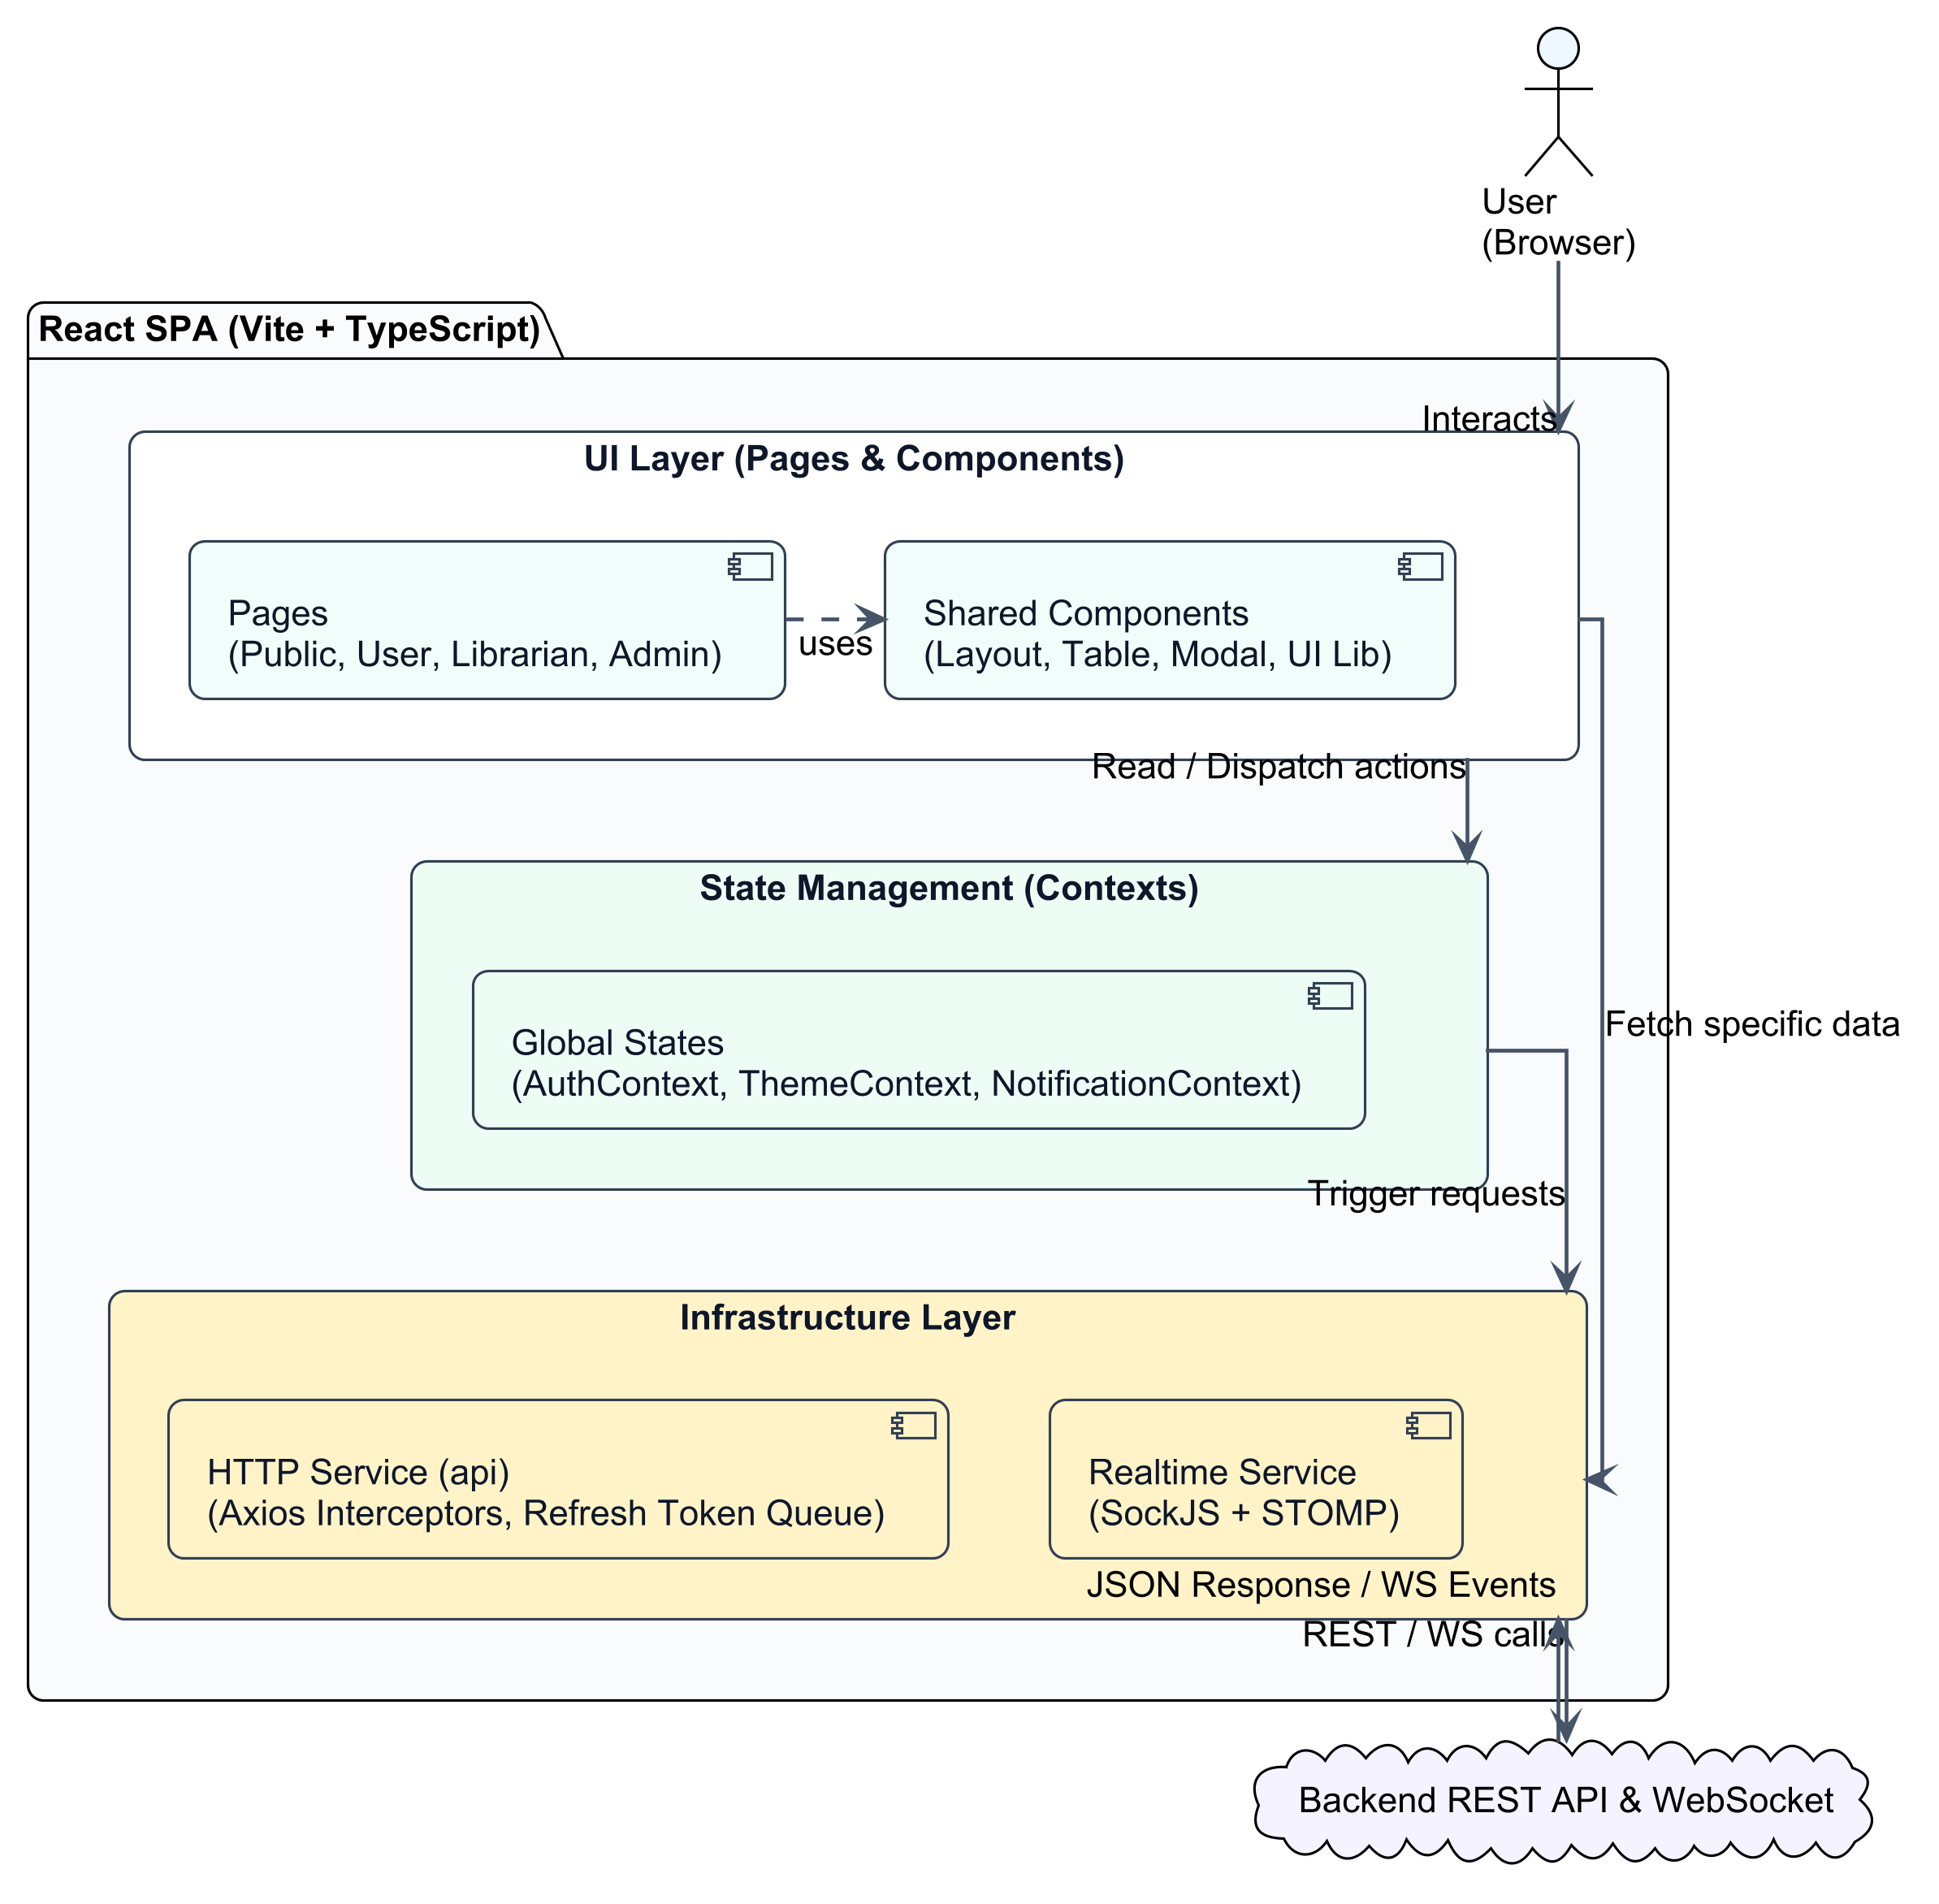
\includegraphics[width=\linewidth]{figures/ch06/frontend/frontend_architecture.png}
        \caption{Sơ đồ kiến trúc và luồng dữ liệu Frontend}
    \end{subfigure}
    \hfill
    \begin{subfigure}[b]{0.3\textwidth}
        \centering
        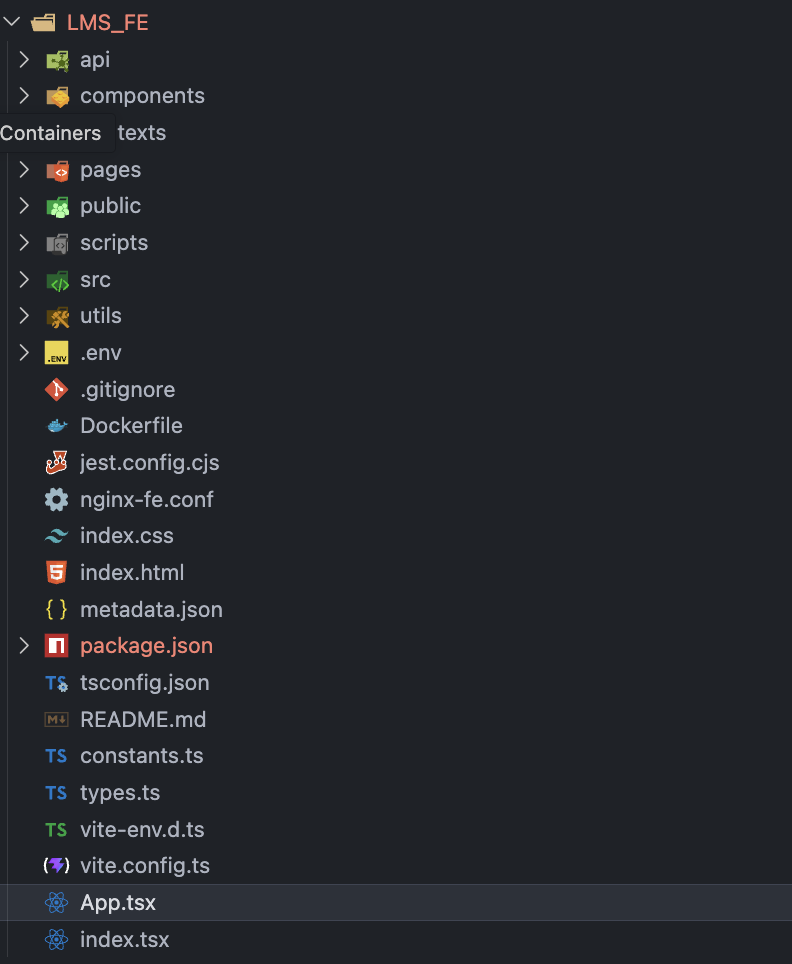
\includegraphics[width=\linewidth]{figures/ch06/frontend/frontend_folder_tree.png}
        \caption{Cấu trúc thư mục \texttt{src} thực tế}
    \end{subfigure}
    \caption{Kiến trúc tổng thể và cách thức tổ chức mã nguồn Frontend}
    \label{fig:fe_architecture_and_structure}
\end{figure}

Dựa trên nền tảng kiến trúc vững chắc này, hệ thống đã triển khai thành công các luồng nghiệp vụ phức tạp và phân định rạch ròi quyền truy cập thông qua cơ chế Route Protection. Bảng \ref{tab:fe_pages_implemented} liệt kê chi tiết danh sách các màn hình chức năng đã được hiện thực và phân quyền cụ thể cho từng nhóm người dùng (Bạn đọc, Thủ thư, Quản trị viên).

\begin{longtable}{|p{2.9cm}|p{4.2cm}|p{7.2cm}|}
\caption{Các màn hình Frontend đã hiện thực theo nhóm người dùng}
\label{tab:fe_pages_implemented}\\
\hline
\textbf{Nhóm trang} & \textbf{Màn hình} & \textbf{Chức năng đã hiện thực} \\
\hline
\endfirsthead
\hline
\textbf{Nhóm trang} & \textbf{Màn hình} & \textbf{Chức năng đã hiện thực} \\
\hline
\endhead
\texttt{/publicpage} & Trang chủ &
Hiển thị sách mới, sách được mượn nhiều, sách được đánh giá cao, thống kê công
khai và ô tìm kiếm nhanh. \\
\hline
\texttt{/publicpage} & Tìm kiếm sách &
Tìm kiếm theo từ khóa, lọc danh mục/tag/ngôn ngữ/năm xuất bản/trạng thái bản
sao, sắp xếp, phân trang và chuyển sang semantic search khi cần. \\
\hline
\texttt{/publicpage} & Chi tiết sách &
Hiển thị metadata, bản sao, trạng thái khả dụng, summary/tag AI, rating, review,
sách tương tự, nút mượn hoặc đặt trước. \\
\hline
\texttt{/publicpage} & Auth pages &
Đăng ký, đăng nhập, Google OAuth callback, xác thực email, quên mật khẩu và đặt
lại mật khẩu. \\
\hline
\texttt{/publicpage} & Liên hệ, hướng dẫn, FAQ &
Hiển thị thông tin thư viện, form liên hệ, iframe Google Maps lazy loading và
nội dung hướng dẫn sử dụng. \\
\hline
\texttt{/userpage} & Dashboard bạn đọc &
Tổng hợp sách đang mượn, đặt trước, phí phạt, thông báo, gợi ý sách và thao tác
nhanh. \\
\hline
\texttt{/userpage} & Sách đang mượn/lịch sử &
Theo dõi giao dịch mượn, hạn trả, trạng thái quá hạn, lịch sử mượn trả và chi
tiết giao dịch. \\
\hline
\texttt{/userpage} & Đặt trước &
Xem danh sách phiếu đặt trước, vị trí hàng chờ, trạng thái sẵn sàng nhận sách,
deadline và hủy đặt trước. \\
\hline
\texttt{/userpage} & Phí phạt &
Xem phí quá hạn/hư/mất, trạng thái thanh toán, tạo QR PayOS và cập nhật kết quả
thanh toán. \\
\hline
\texttt{/userpage} & Wishlist, rating, hồ sơ &
Lưu sách yêu thích, đánh giá sách sau khi mượn, phản hồi review, cập nhật hồ sơ,
avatar, mật khẩu, ngôn ngữ và theme. \\
\hline
\texttt{/userpage} & Thông báo &
Nhận thông báo realtime, đánh dấu đã đọc, xem thông báo về mượn--trả, đặt trước,
phí phạt và phản hồi review. \\
\hline
\texttt{/librarianpage} & Dashboard thủ thư &
Thống kê vận hành, sách mượn/trả, yêu cầu chờ xử lý, phí phạt, cảnh báo quá hạn
và các thao tác nhanh. \\
\hline
\texttt{/librarianpage} & Quản lý ấn phẩm &
Tạo/sửa/xóa ấn phẩm, tác giả, nhà xuất bản, danh mục, tag, ảnh bìa, ISBN auto
fill, upload PDF và theo dõi trạng thái xử lý AI. \\
\hline
\texttt{/librarianpage} & Quản lý bản sao &
Tạo bản sao vật lý, barcode, vị trí kệ, chi nhánh, trạng thái khả dụng, hư/mất
và lịch sử lưu thông. \\
\hline
\texttt{/librarianpage} & Mượn--trả tại quầy &
Tra cứu bạn đọc, quét/nhập barcode, cho mượn trực tiếp, xác nhận nhận sách, trả
sách, ghi chú giao dịch và xử lý sách hư/mất. \\
\hline
\texttt{/librarianpage} & Yêu cầu và đặt trước &
Xem yêu cầu mượn, duyệt/từ chối, quản lý hàng chờ đặt trước, xác nhận nhận sách
và gửi thông báo cho bạn đọc. \\
\hline
\texttt{/librarianpage} & Phí phạt và thanh toán &
Tính phí, thu tiền mặt, tạo QR PayOS, polling trạng thái chuyển khoản và cập
nhật trạng thái fine. \\
\hline
\texttt{/adminpage} & Quản lý tài khoản &
Quản lý tài khoản độc giả/thủ thư, tạo thủ thư, khóa/mở khóa, xác minh tài
khoản và cập nhật trạng thái người dùng. \\
\hline
\texttt{/adminpage} & Chính sách và audit &
Cấu hình quy định mượn trả, xem nhật ký thao tác, lọc audit log và theo dõi thay
đổi vận hành hệ thống. \\
\hline
\end{longtable}

% ==========================================
% 1. PHÂN HỆ BẠN ĐỌC (READER FLOW)
% ==========================================
Để mang lại trải nghiệm liền mạch cho bạn đọc, phân hệ Frontend được thiết kế tối ưu từ khâu khám phá tài liệu đến các thao tác tương tác chi tiết. Quá trình này bắt đầu tại màn hình Dashboard và công cụ tìm kiếm ngữ nghĩa, nơi người dùng có thể tra cứu ấn phẩm bằng ngôn ngữ tự nhiên thay vì chỉ dựa vào từ khóa rập khuôn.

\begin{figure}[H]
    \centering
    \begin{subfigure}[b]{0.48\textwidth}
        \centering
        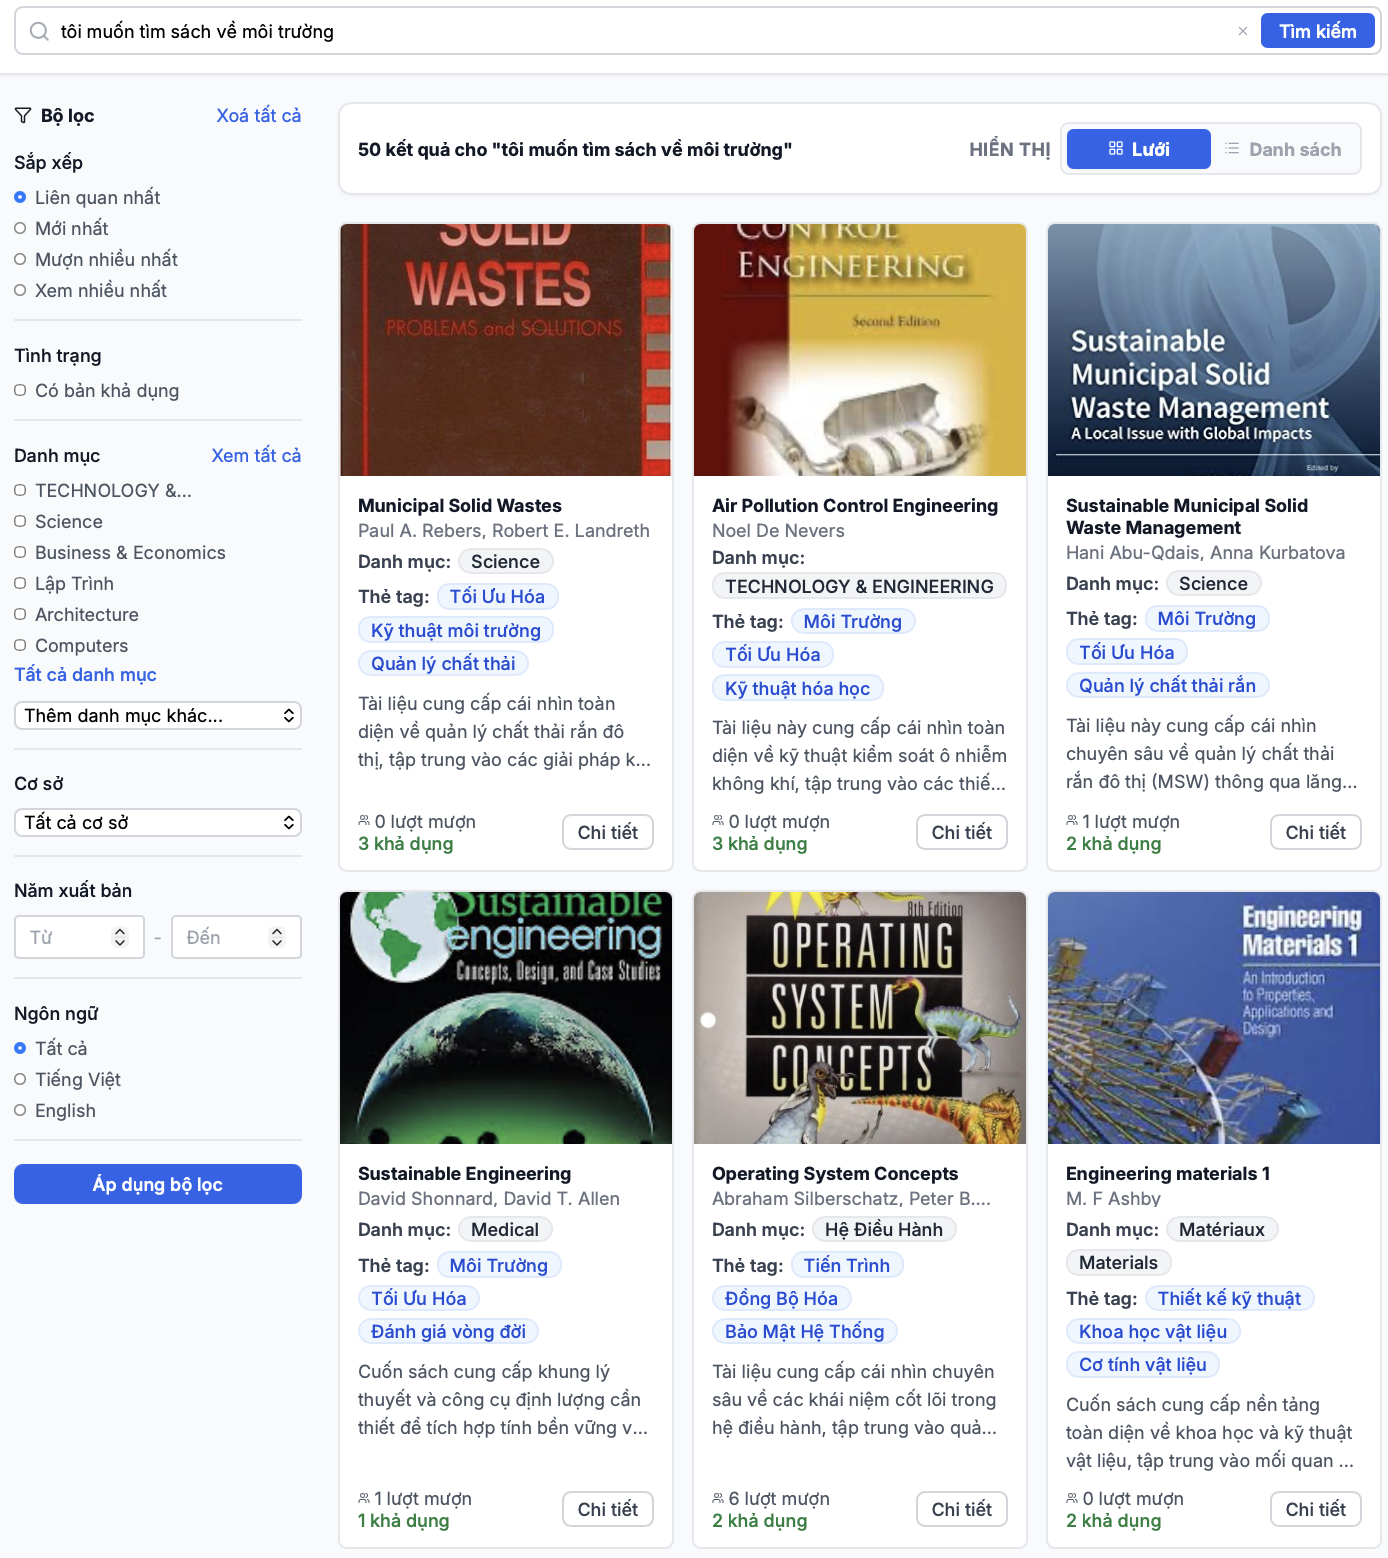
\includegraphics[width=\linewidth]{figures/ch06/frontend/semantic_search_page.png}
        \caption{Tìm kiếm ngữ nghĩa và lọc sách}
    \end{subfigure}
    \hfill
    \begin{subfigure}[b]{0.48\textwidth}
        \centering
        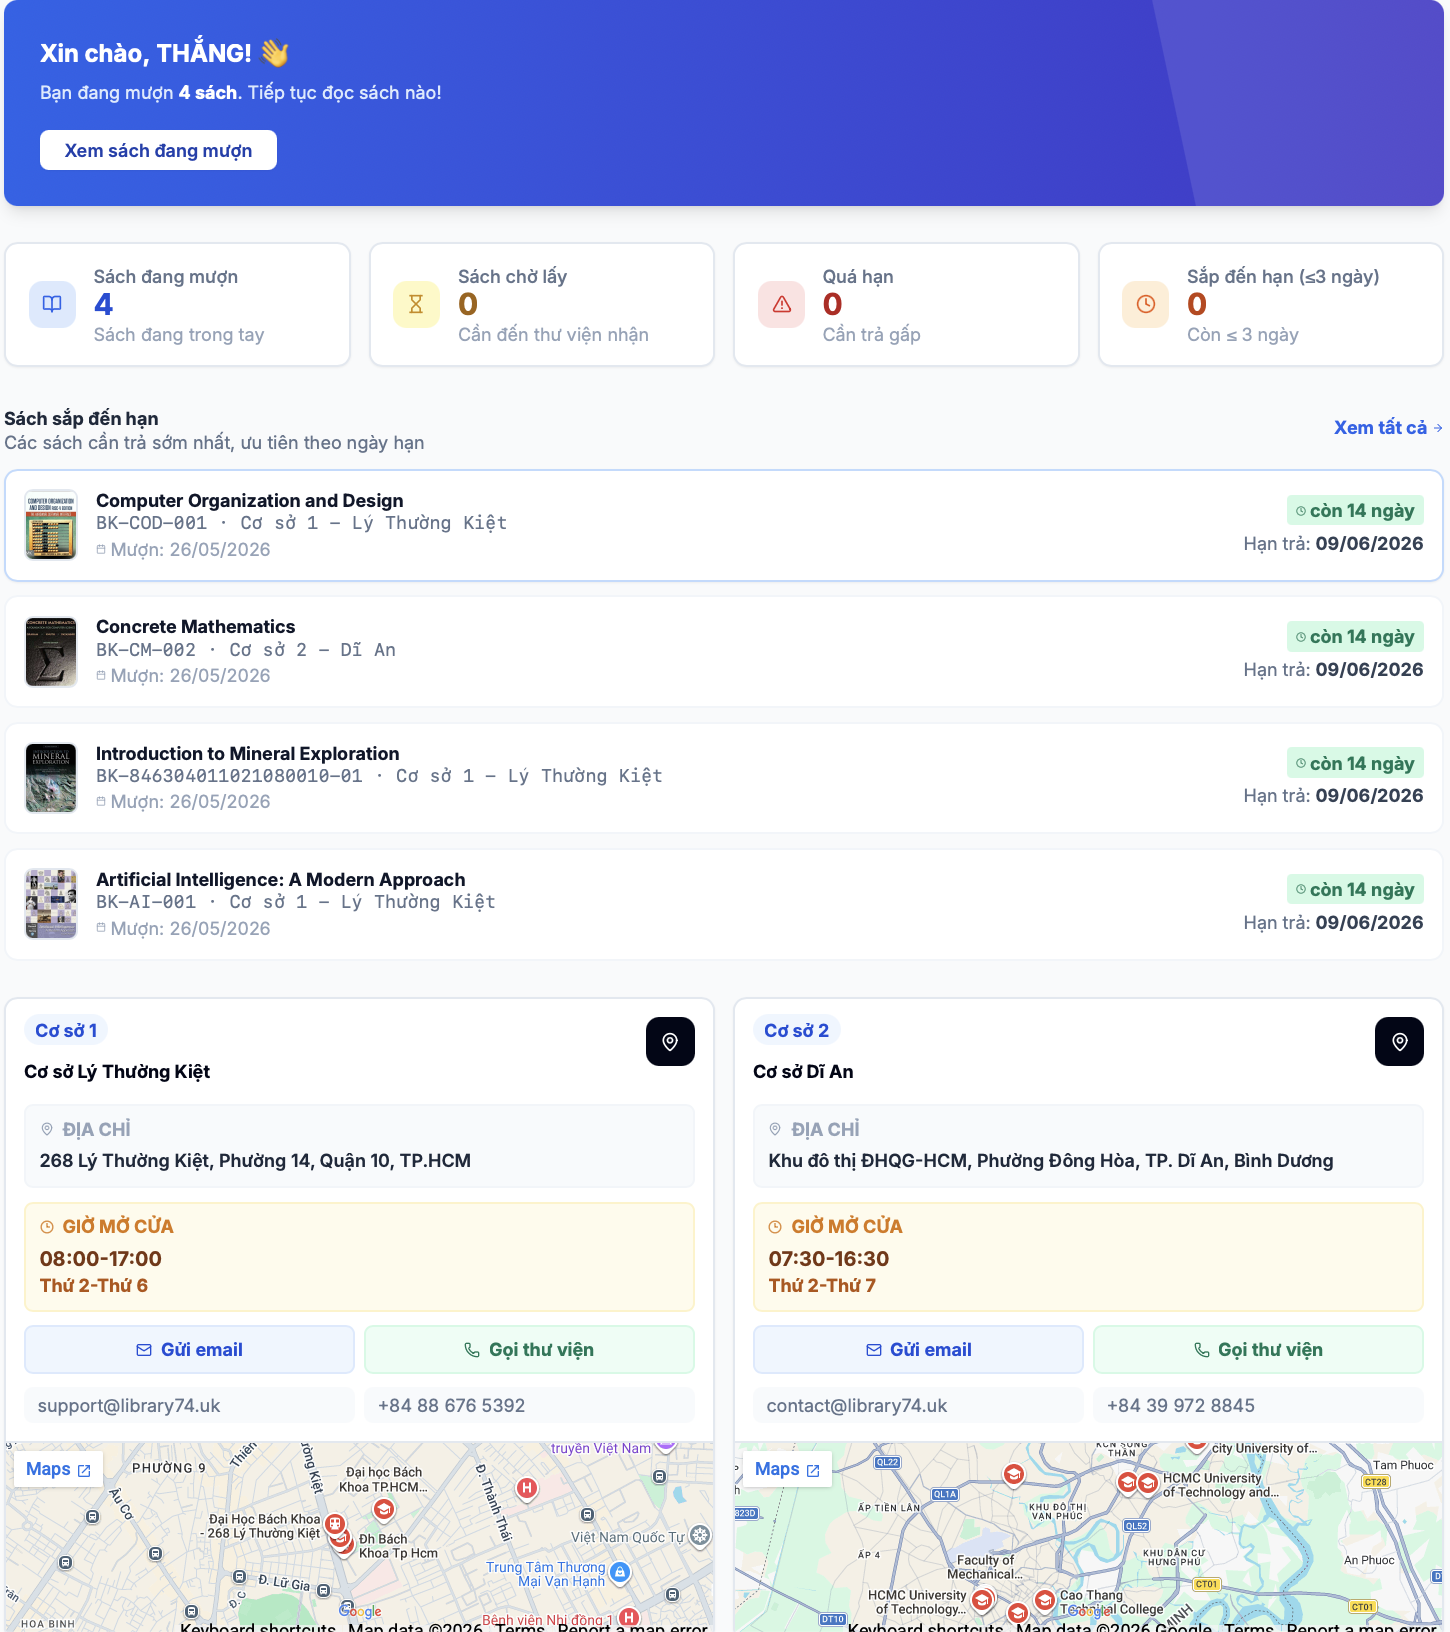
\includegraphics[width=\linewidth]{figures/ch06/frontend/reader_dashboard.png}
        \caption{Dashboard bạn đọc}
    \end{subfigure}
    \caption{Giao diện tổng quan và chức năng tìm kiếm thông minh dành cho bạn đọc}
    \label{fig:fe_reader_discovery}
\end{figure}

Sau khi tìm được tài liệu mong muốn, bạn đọc có thể xem thông tin chi tiết với các siêu dữ liệu (metadata) được AI tự động trích xuất. Đồng thời, hệ thống cung cấp đầy đủ các tính năng tương tác như đánh giá, phản hồi và thanh toán trực tuyến tự động thông qua mã QR PayOS.

\begin{figure}[H]
    \centering
    \begin{subfigure}[b]{0.48\textwidth}
        \centering
        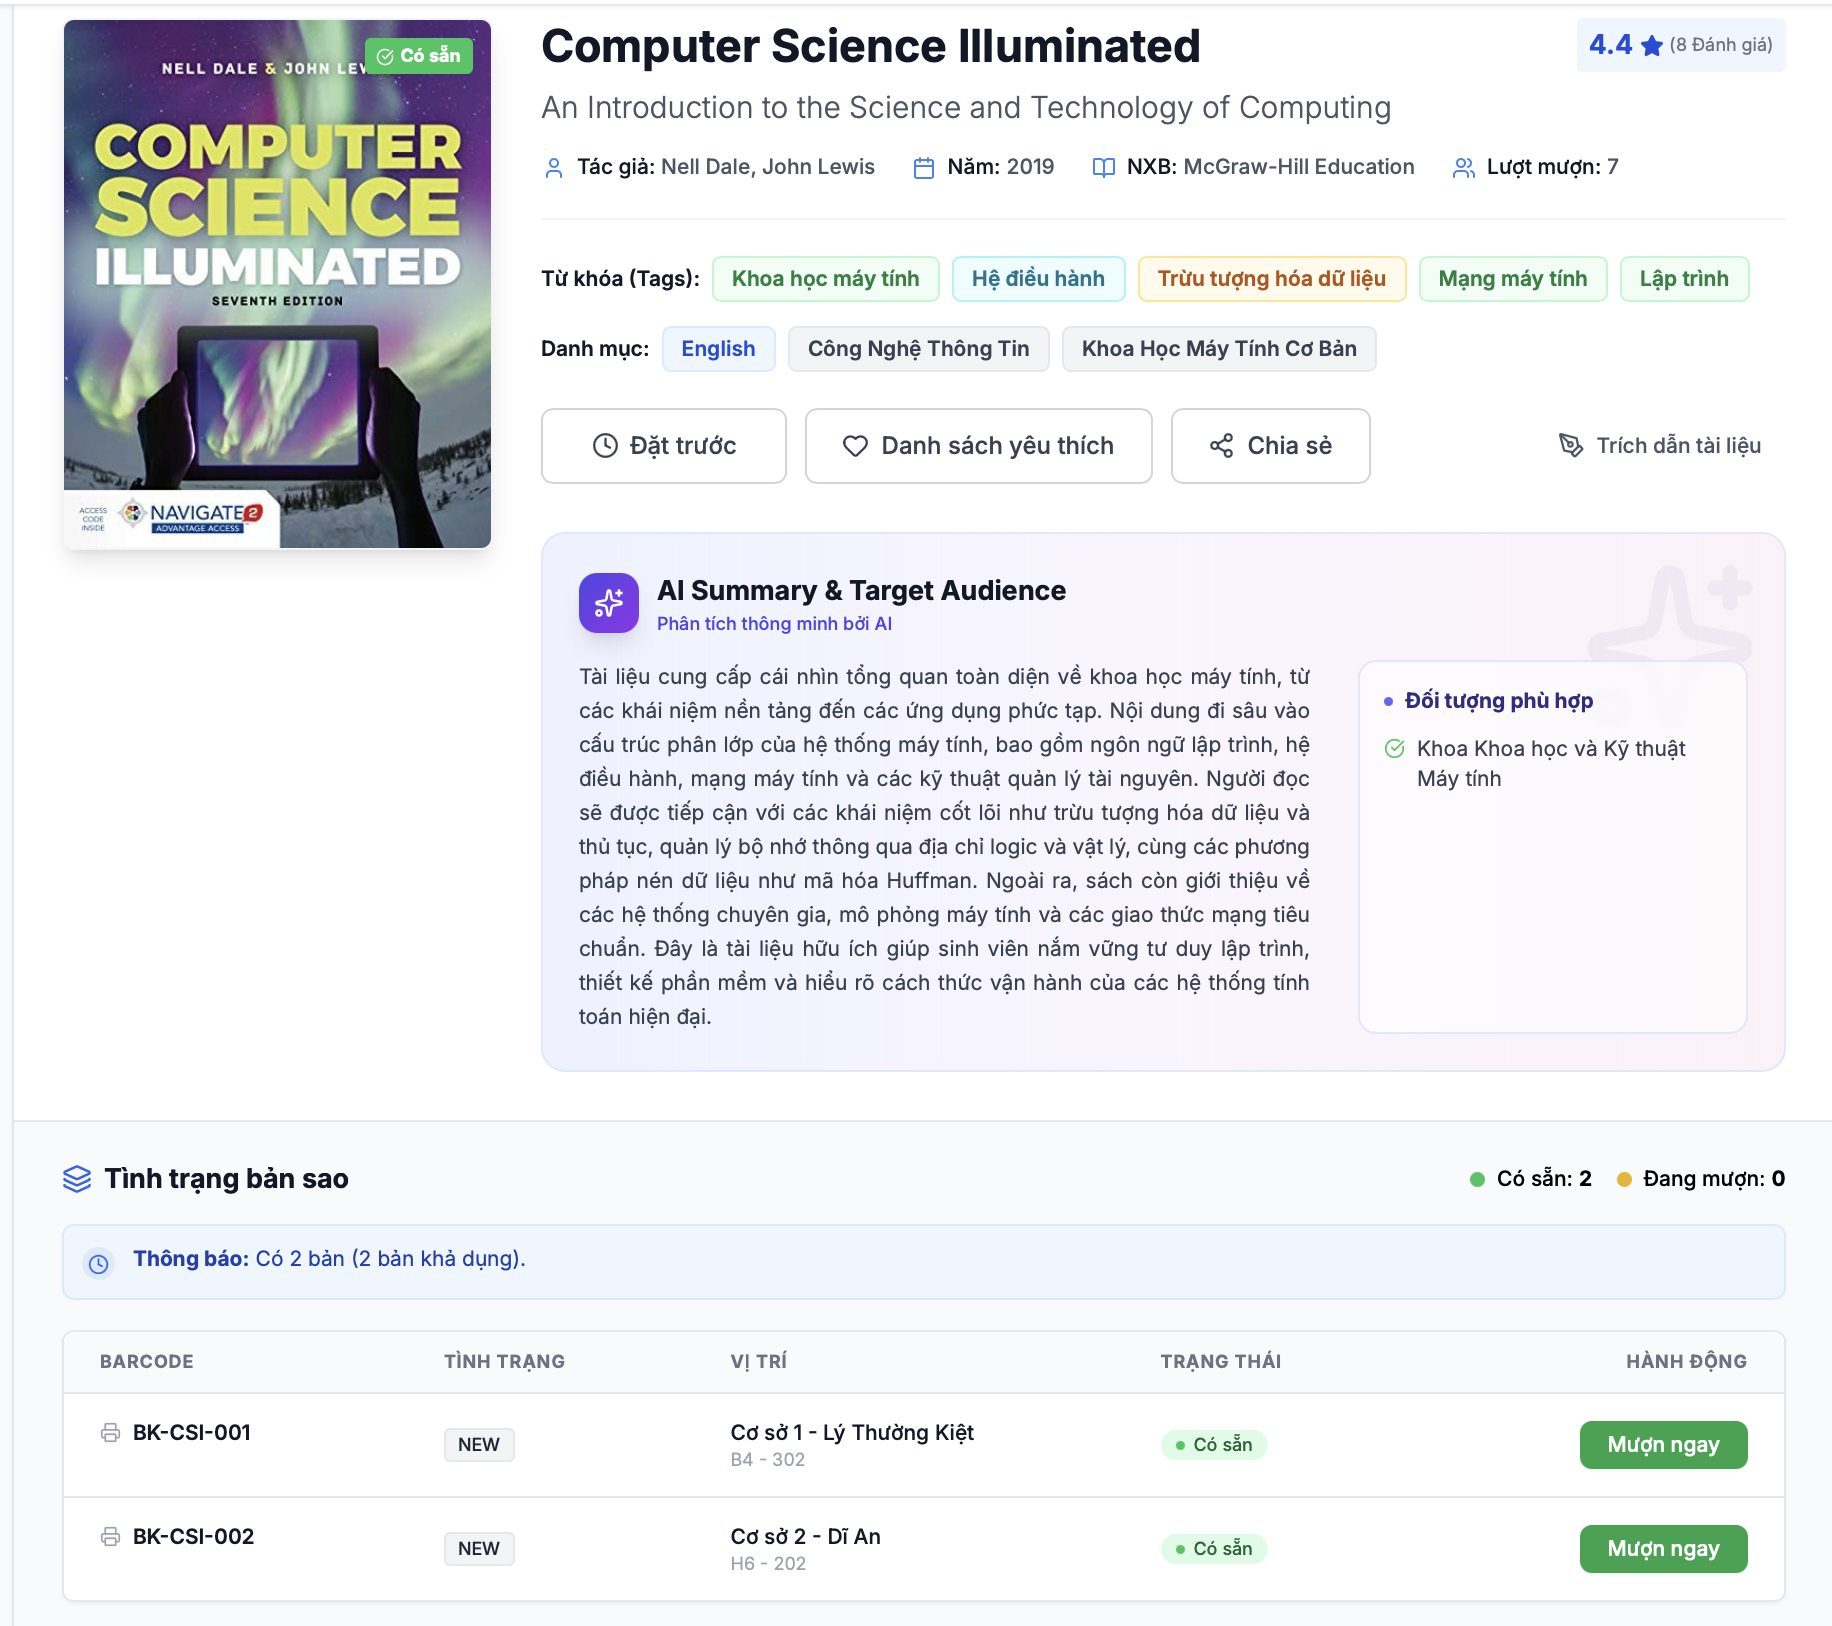
\includegraphics[width=\linewidth]{figures/ch06/frontend/book_detail.png}
        \caption{Chi tiết sách và siêu dữ liệu (metadata) AI}
    \end{subfigure}
    \hfill
    \begin{subfigure}[b]{0.48\textwidth}
        \centering
        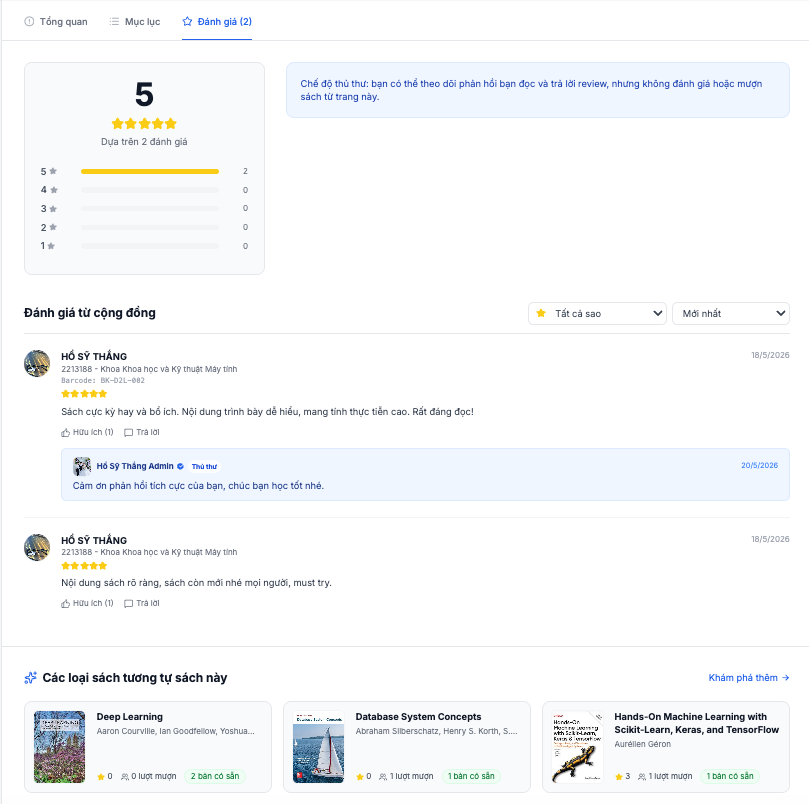
\includegraphics[width=\linewidth]{figures/ch06/frontend/book_rating_review.png}
        \caption{Đánh giá và phản hồi}
    \end{subfigure}
    \caption{Trải nghiệm xem chi tiết và tương tác với ấn phẩm}
    \label{fig:fe_reader_interaction}
\end{figure}

\begin{figure}[H]
    \centering
    \begin{subfigure}[b]{0.48\textwidth}
        \centering
        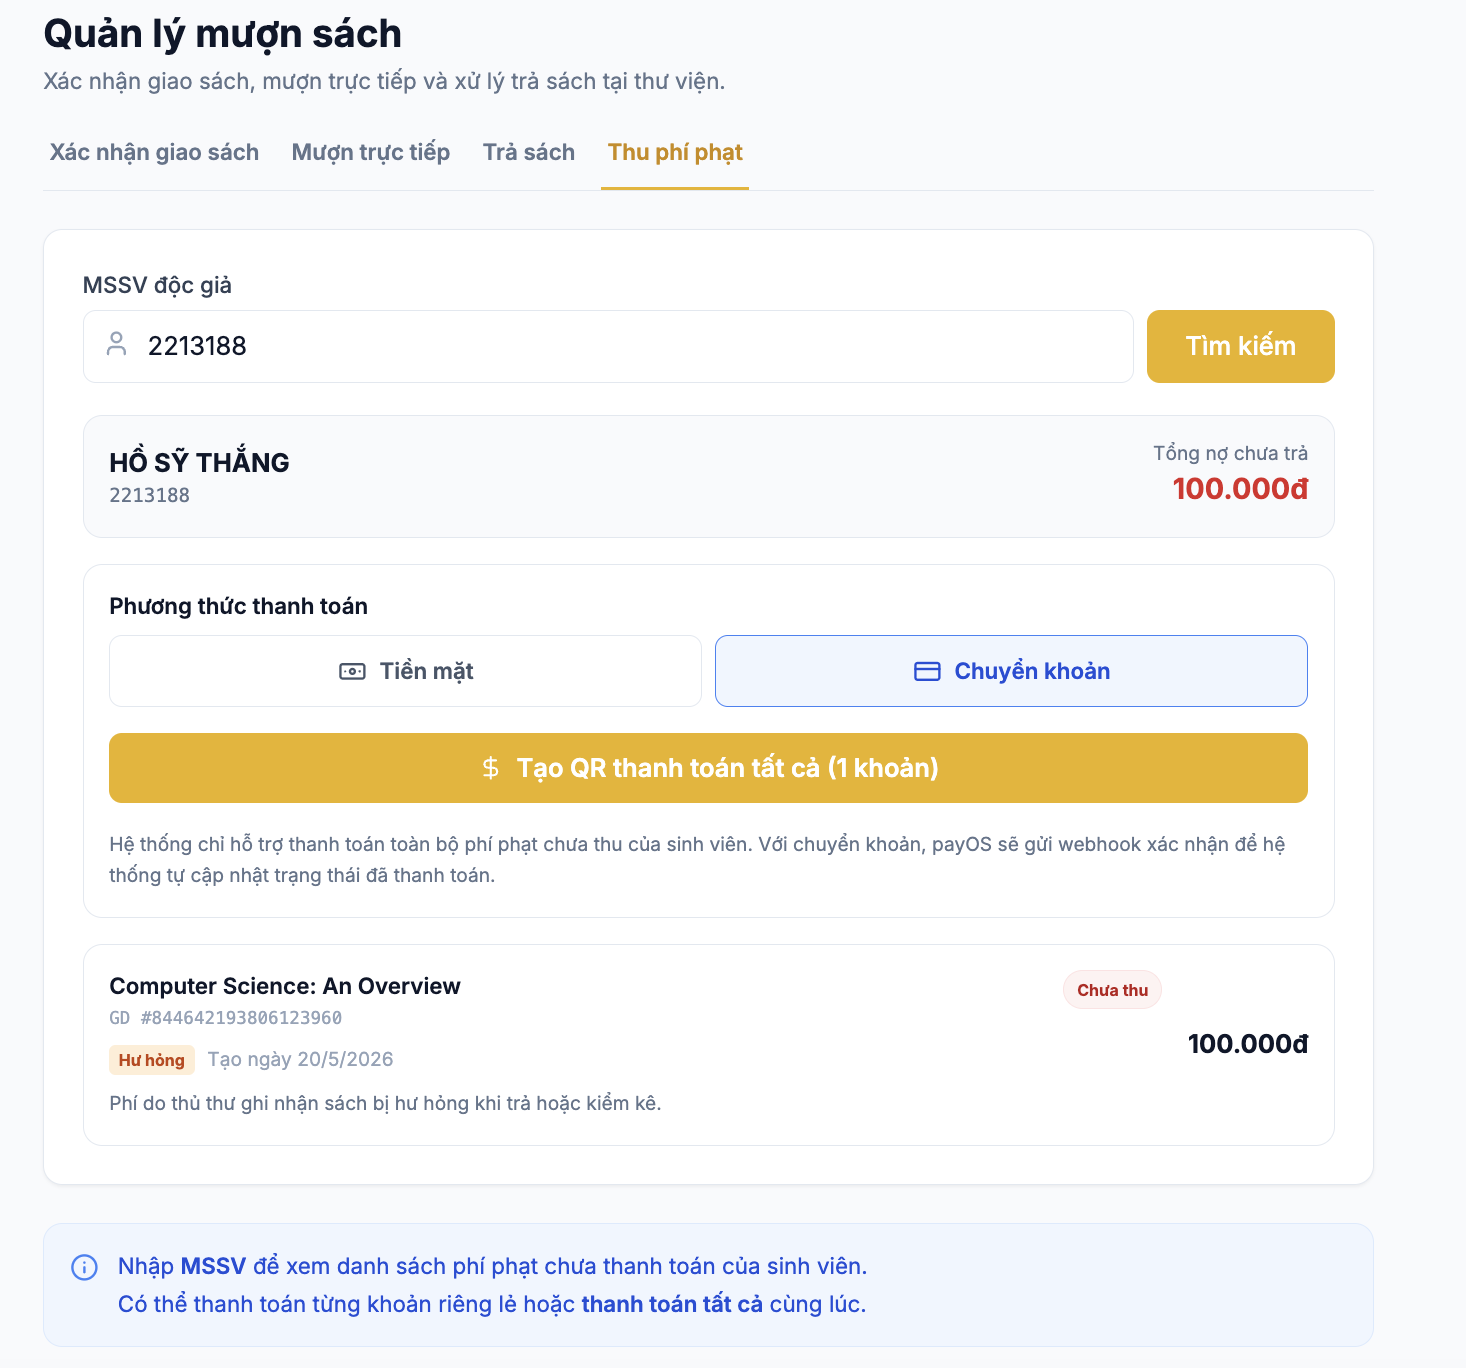
\includegraphics[width=\linewidth]{figures/ch06/payment/init_qr.png}
        \caption{Khởi tạo thanh toán}
    \end{subfigure}
    \hfill
    \begin{subfigure}[b]{0.48\textwidth}
        \centering
        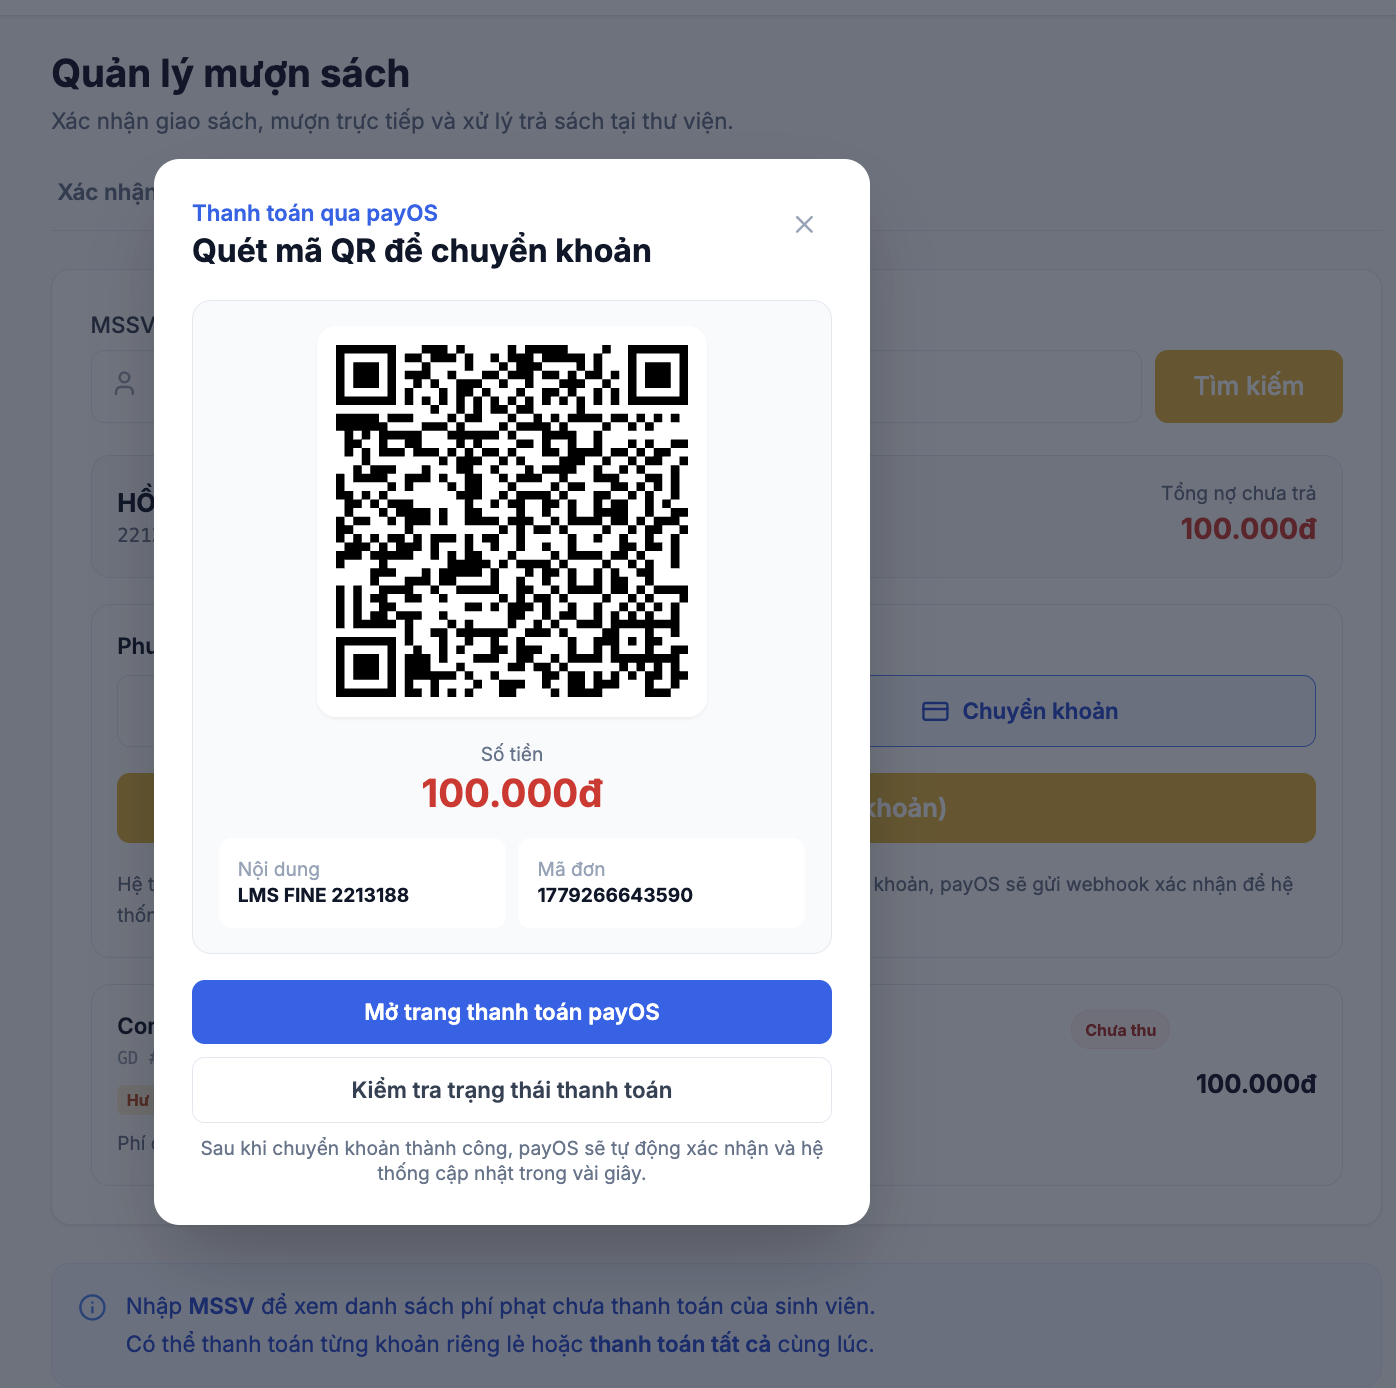
\includegraphics[width=\linewidth]{figures/ch06/payment/create_qr.png}
        \caption{Hiển thị mã QR PayOS}
    \end{subfigure}
    \caption{Quy trình tích hợp thanh toán tự động}
    \label{fig:fe_payment_integration}
\end{figure}

% ==========================================
% 2. PHÂN HỆ THỦ THƯ (LIBRARIAN FLOW)
% ==========================================
Đối với nghiệp vụ quản trị, hệ thống tập trung giải quyết bài toán giảm tải thao tác thủ công cho thủ thư bằng cách tự động hóa luồng số hóa tài liệu. Các tính năng nổi bật bao gồm tự động điền thông tin từ mã ISBN và giám sát tiến trình AI xử lý tài liệu vừa tải lên.

\begin{figure}[H]
    \centering
     \begin{subfigure}[b]{0.48\textwidth}
        \centering
        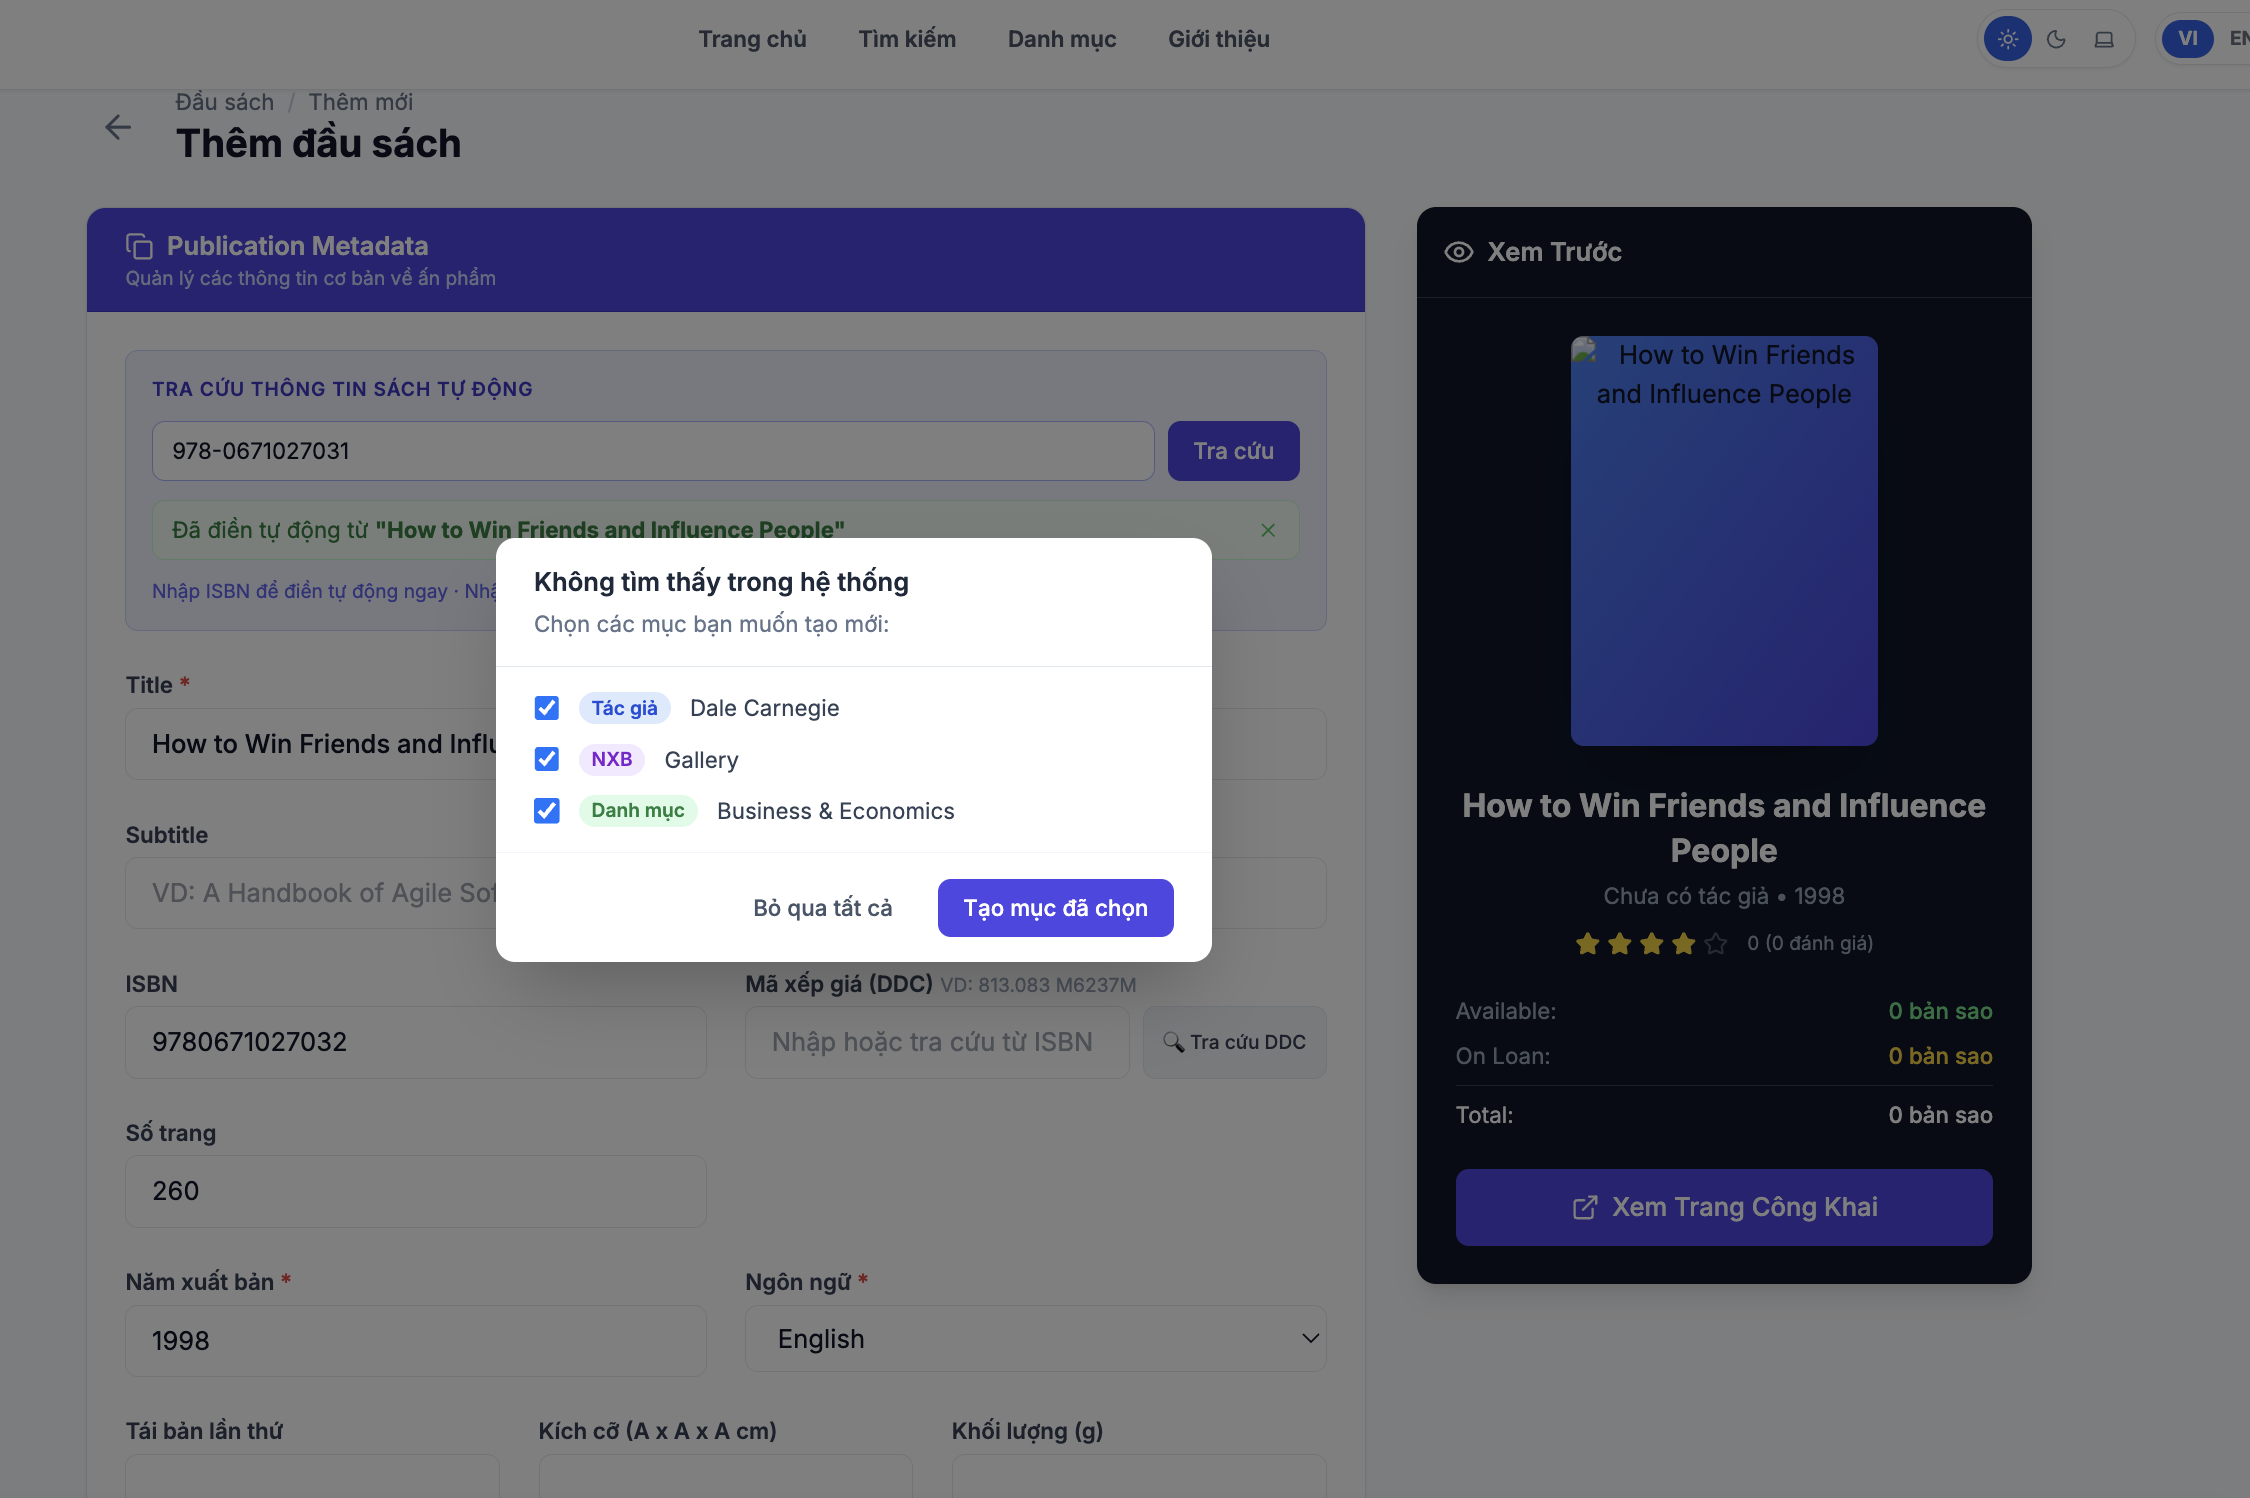
\includegraphics[width=\linewidth]{figures/ch06/frontend/isbn_auto_fill.png}
        \caption{Tự động trích xuất metadata từ ISBN}
    \end{subfigure}
    \hfill
        \begin{subfigure}[b]{0.48\textwidth}
        \centering
        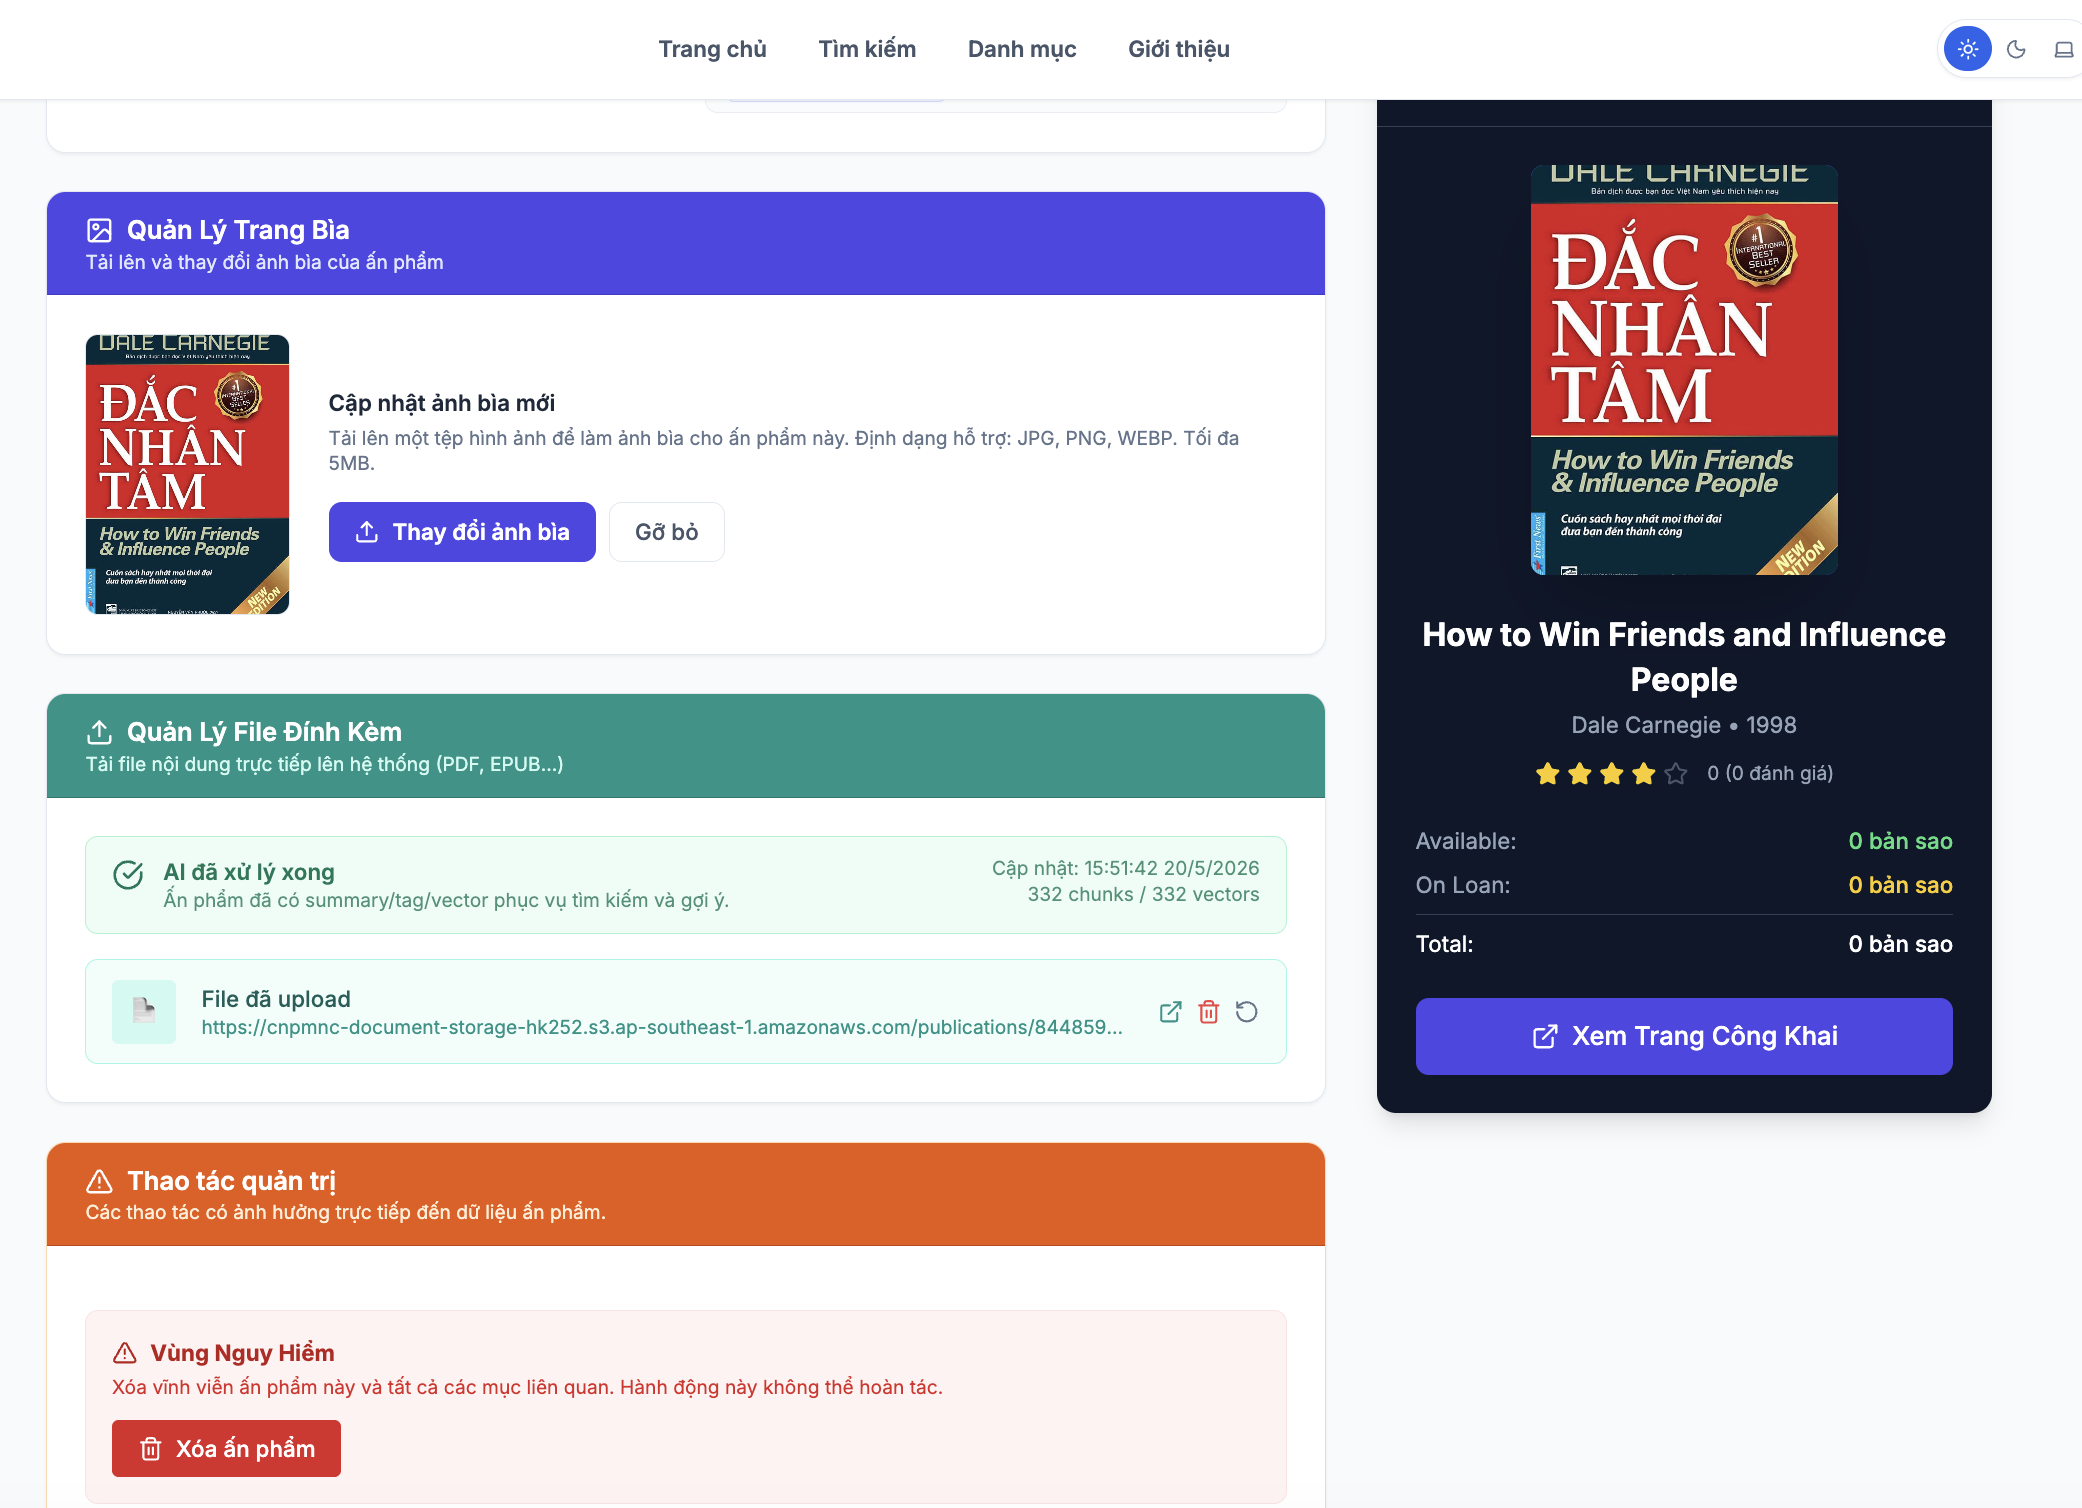
\includegraphics[width=\linewidth]{figures/ch06/frontend/upload_book.png}
        \caption{Tải lên tài liệu và giám sát tiến trình AI}
    \end{subfigure}
    \caption{Nghiệp vụ nhập liệu và số hóa tài liệu thông minh}
    \label{fig:fe_librarian_cataloging}
\end{figure}

Bên cạnh khâu nhập liệu, công tác giám sát và quản lý danh mục ấn phẩm cũng được trực quan hóa, kết hợp cùng hệ thống thông báo thời gian thực (real-time notification) để thủ thư nắm bắt và xử lý kịp thời các sự kiện phát sinh.

\begin{figure}[H]
    \centering
    \begin{subfigure}[b]{0.48\textwidth}
        \centering
        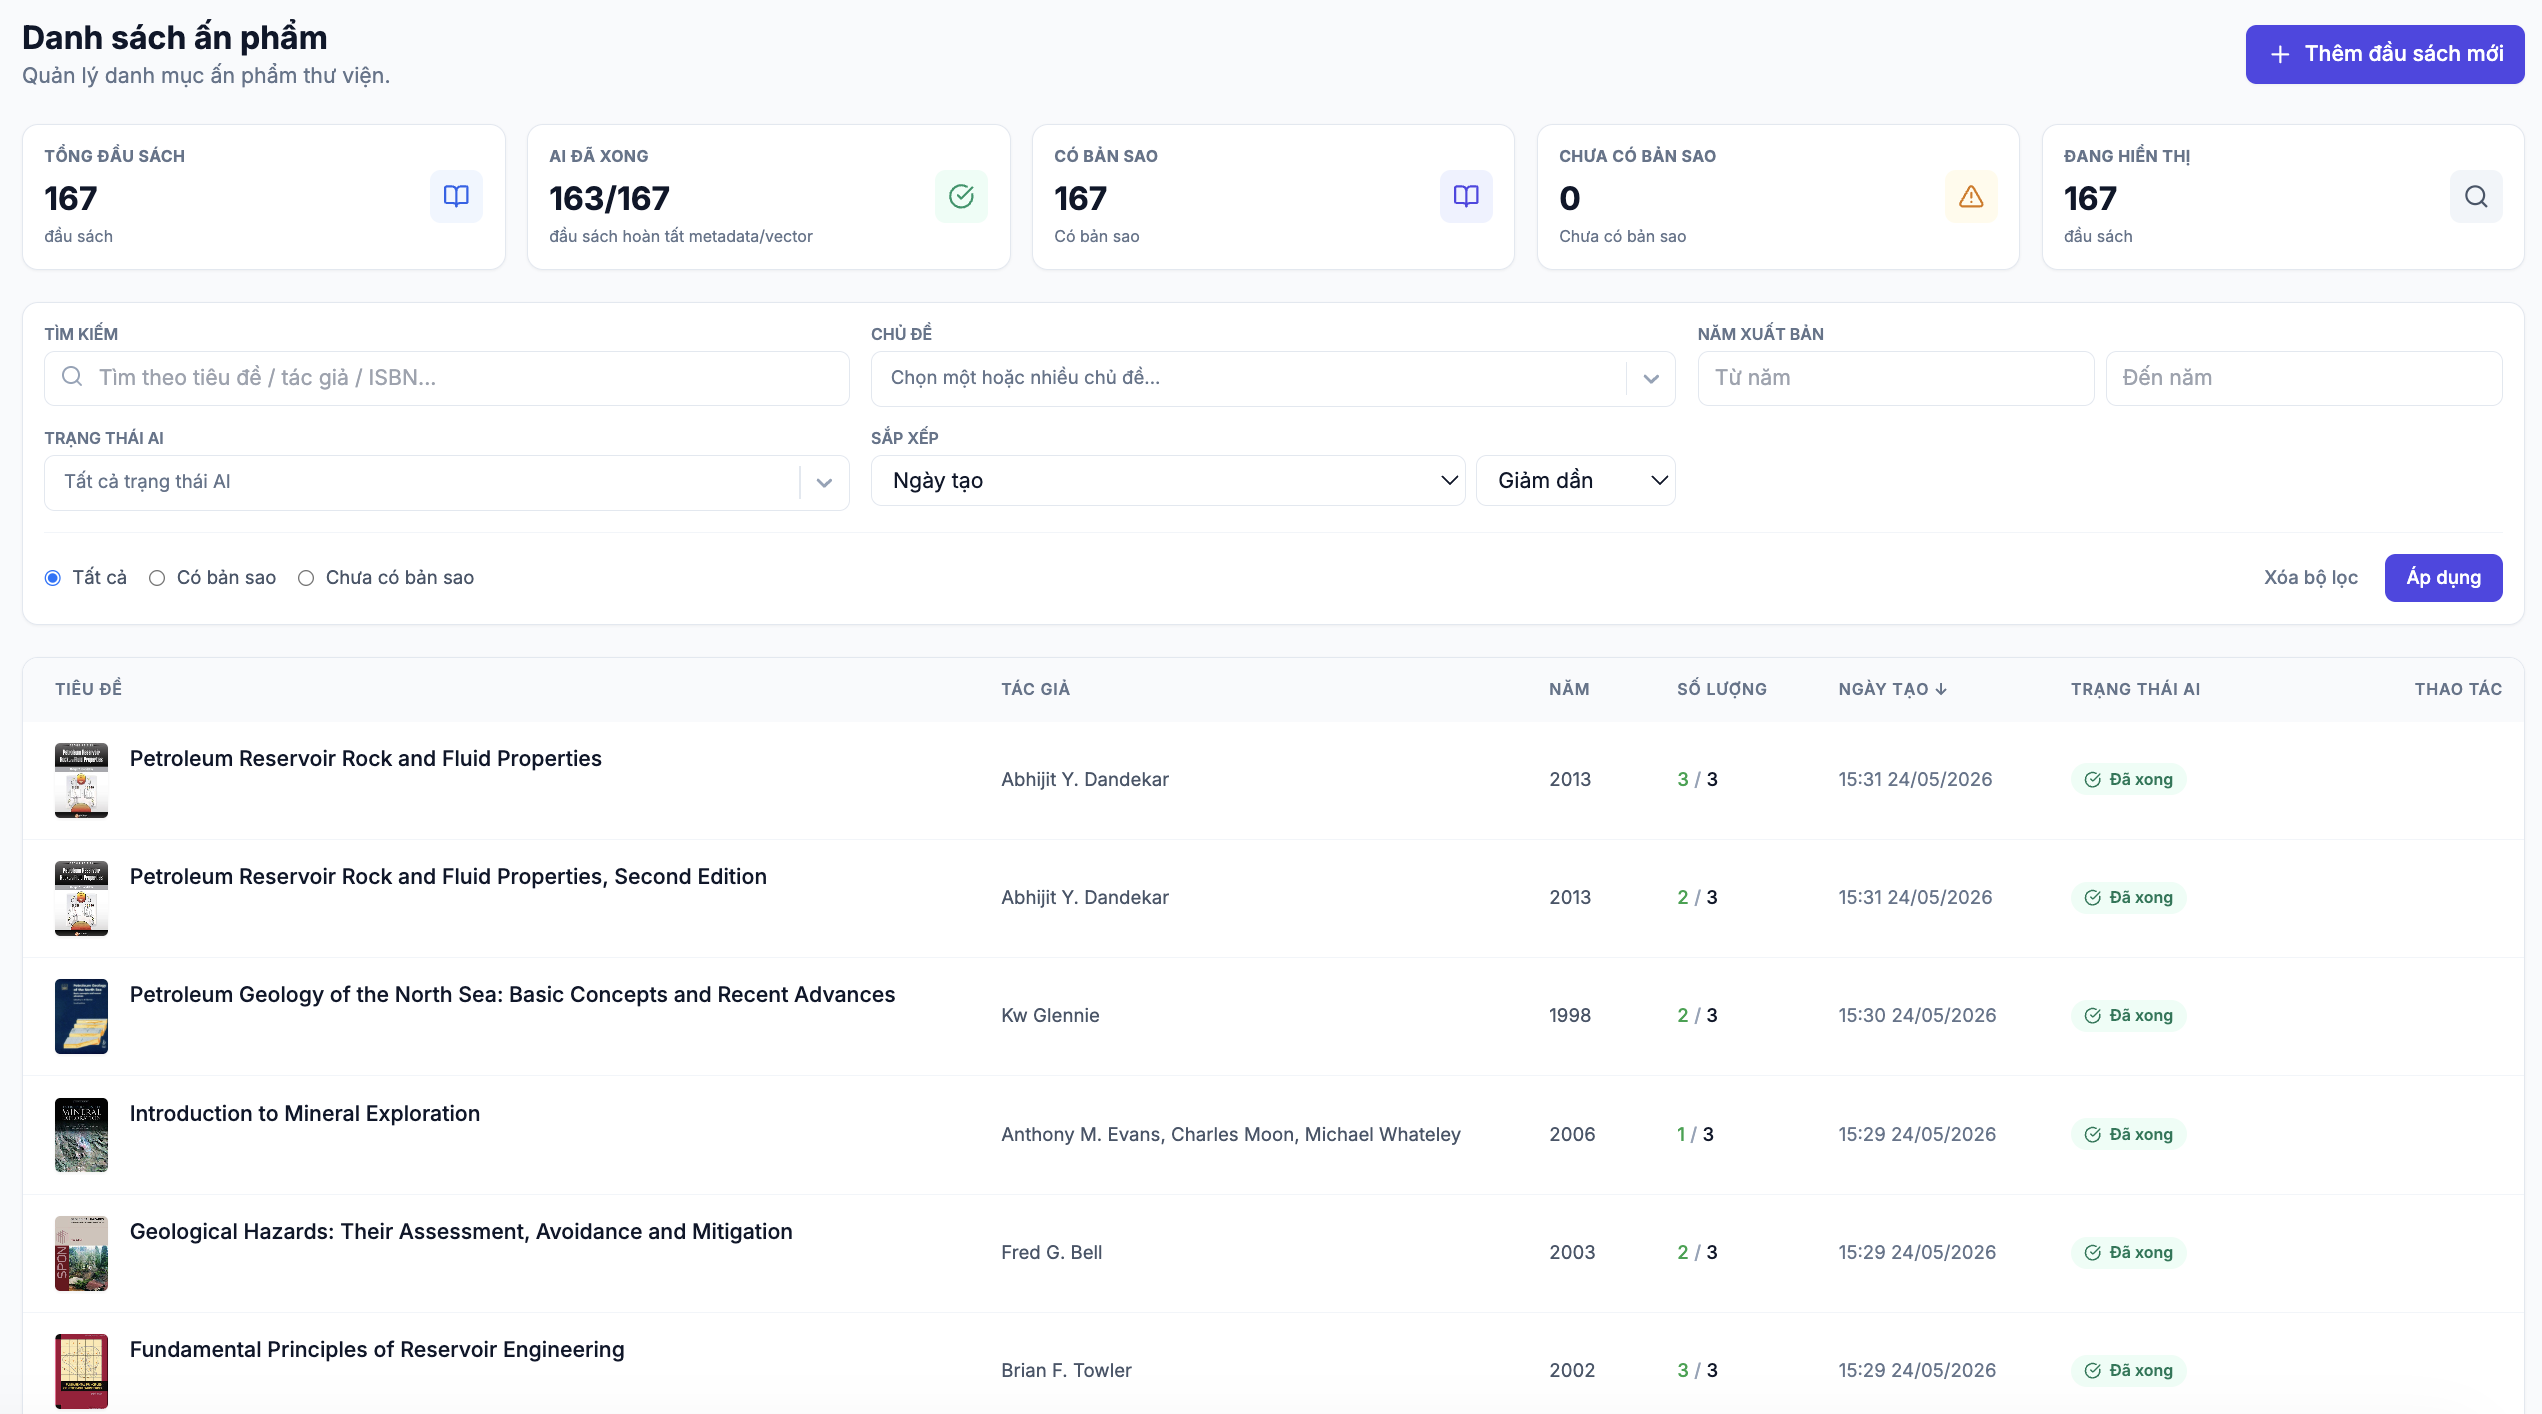
\includegraphics[width=\linewidth]{figures/ch06/frontend/publication_management.png}
        \caption{Quản lý danh mục ấn phẩm}
    \end{subfigure}
    \hfill
        \begin{subfigure}[b]{0.48\textwidth}
        \centering
        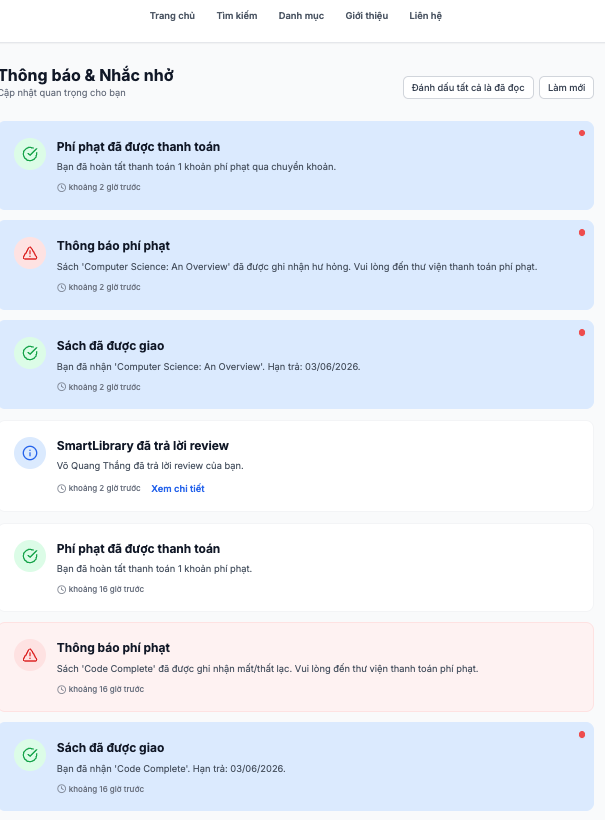
\includegraphics[width=\linewidth]{figures/ch06/frontend/realtime_notification.png}
        \caption{Hệ thống thông báo thời gian thực}
    \end{subfigure}
    \caption{Nghiệp vụ quản lý vận hành và giám sát hệ thống của thủ thư}
    \label{fig:fe_librarian_management}
\end{figure}

% ==========================================
% 3. GIAO TIẾP VÀ CẤU HÌNH HỆ THỐNG
% ==========================================
Cuối cùng, để đảm bảo tính kết nối và đáp ứng đa dạng nhu cầu sử dụng, hệ thống cung cấp luồng giao tiếp hỗ trợ trực tuyến giữa các nhóm người dùng, đi kèm các tùy chọn cá nhân hóa sâu về giao diện (Light/Dark mode) và ngôn ngữ (Việt - Anh).

\begin{figure}[H]
    \centering
    \begin{subfigure}[b]{0.48\textwidth}
        \centering
        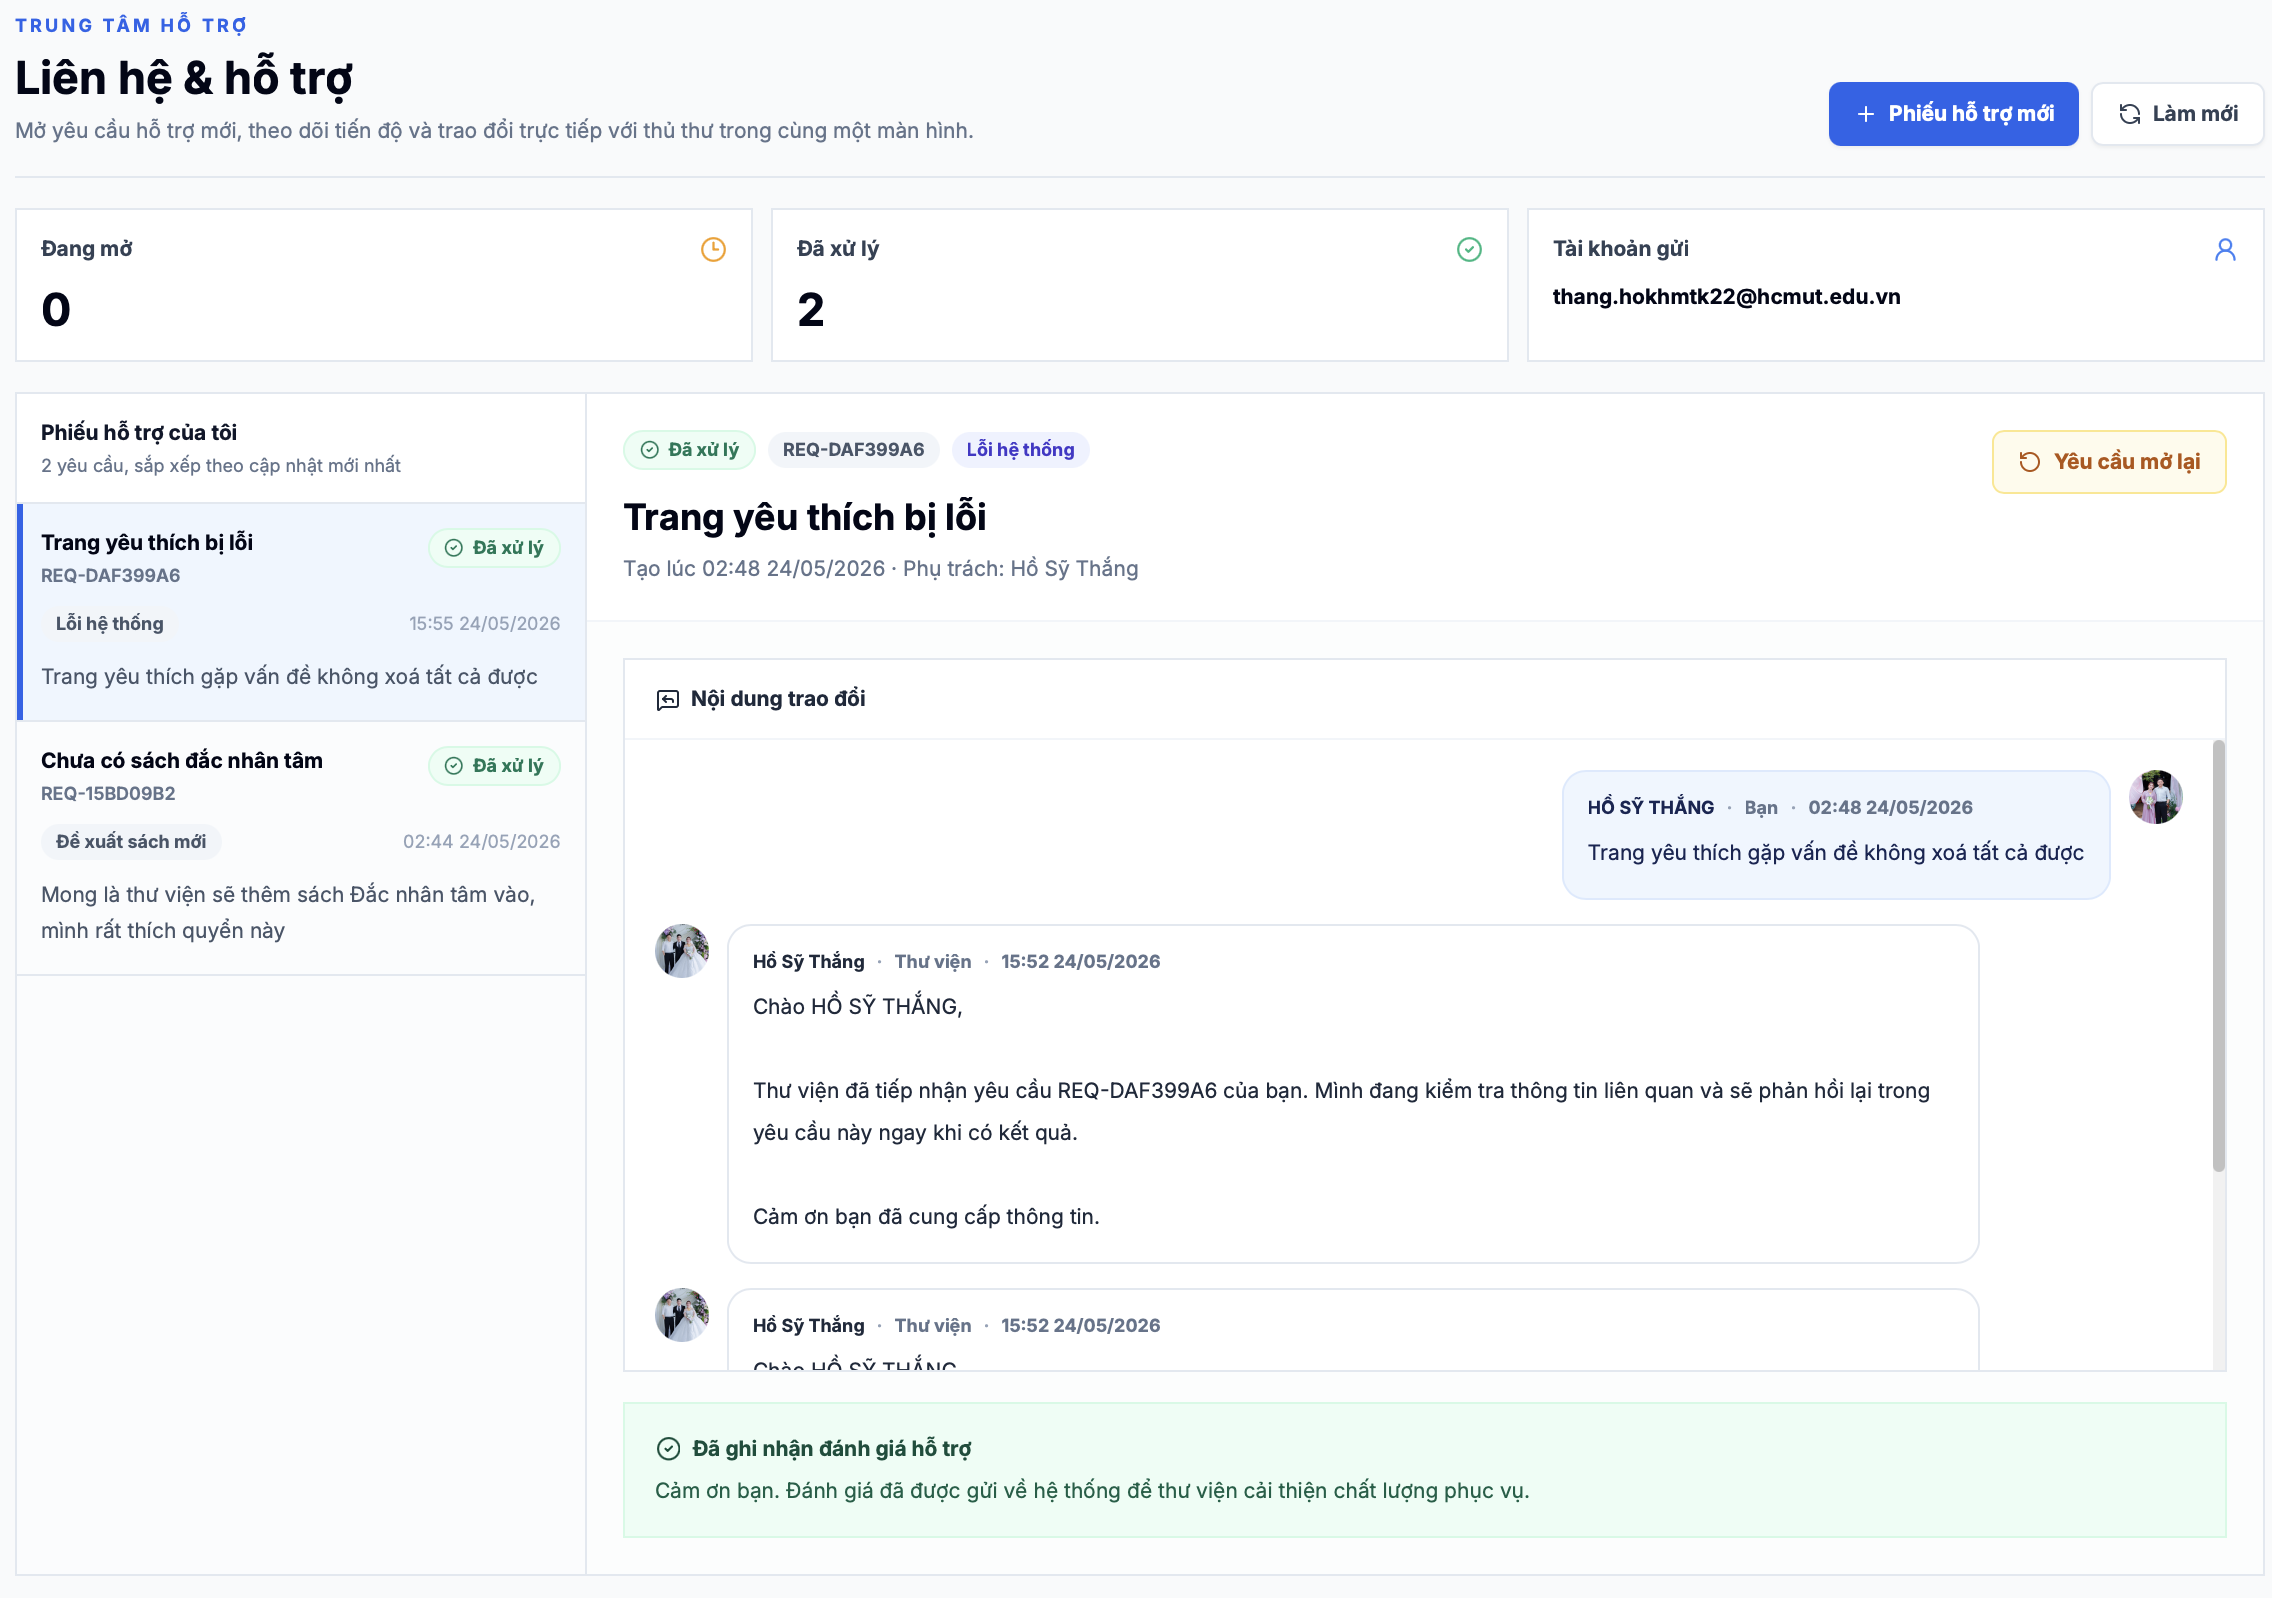
\includegraphics[width=\linewidth]{figures/ch06/frontend/contact_and_support_user.png}
        \caption{Gửi yêu cầu hỗ trợ (Bạn đọc)}
    \end{subfigure}
    \hfill
    \begin{subfigure}[b]{0.48\textwidth}
        \centering
        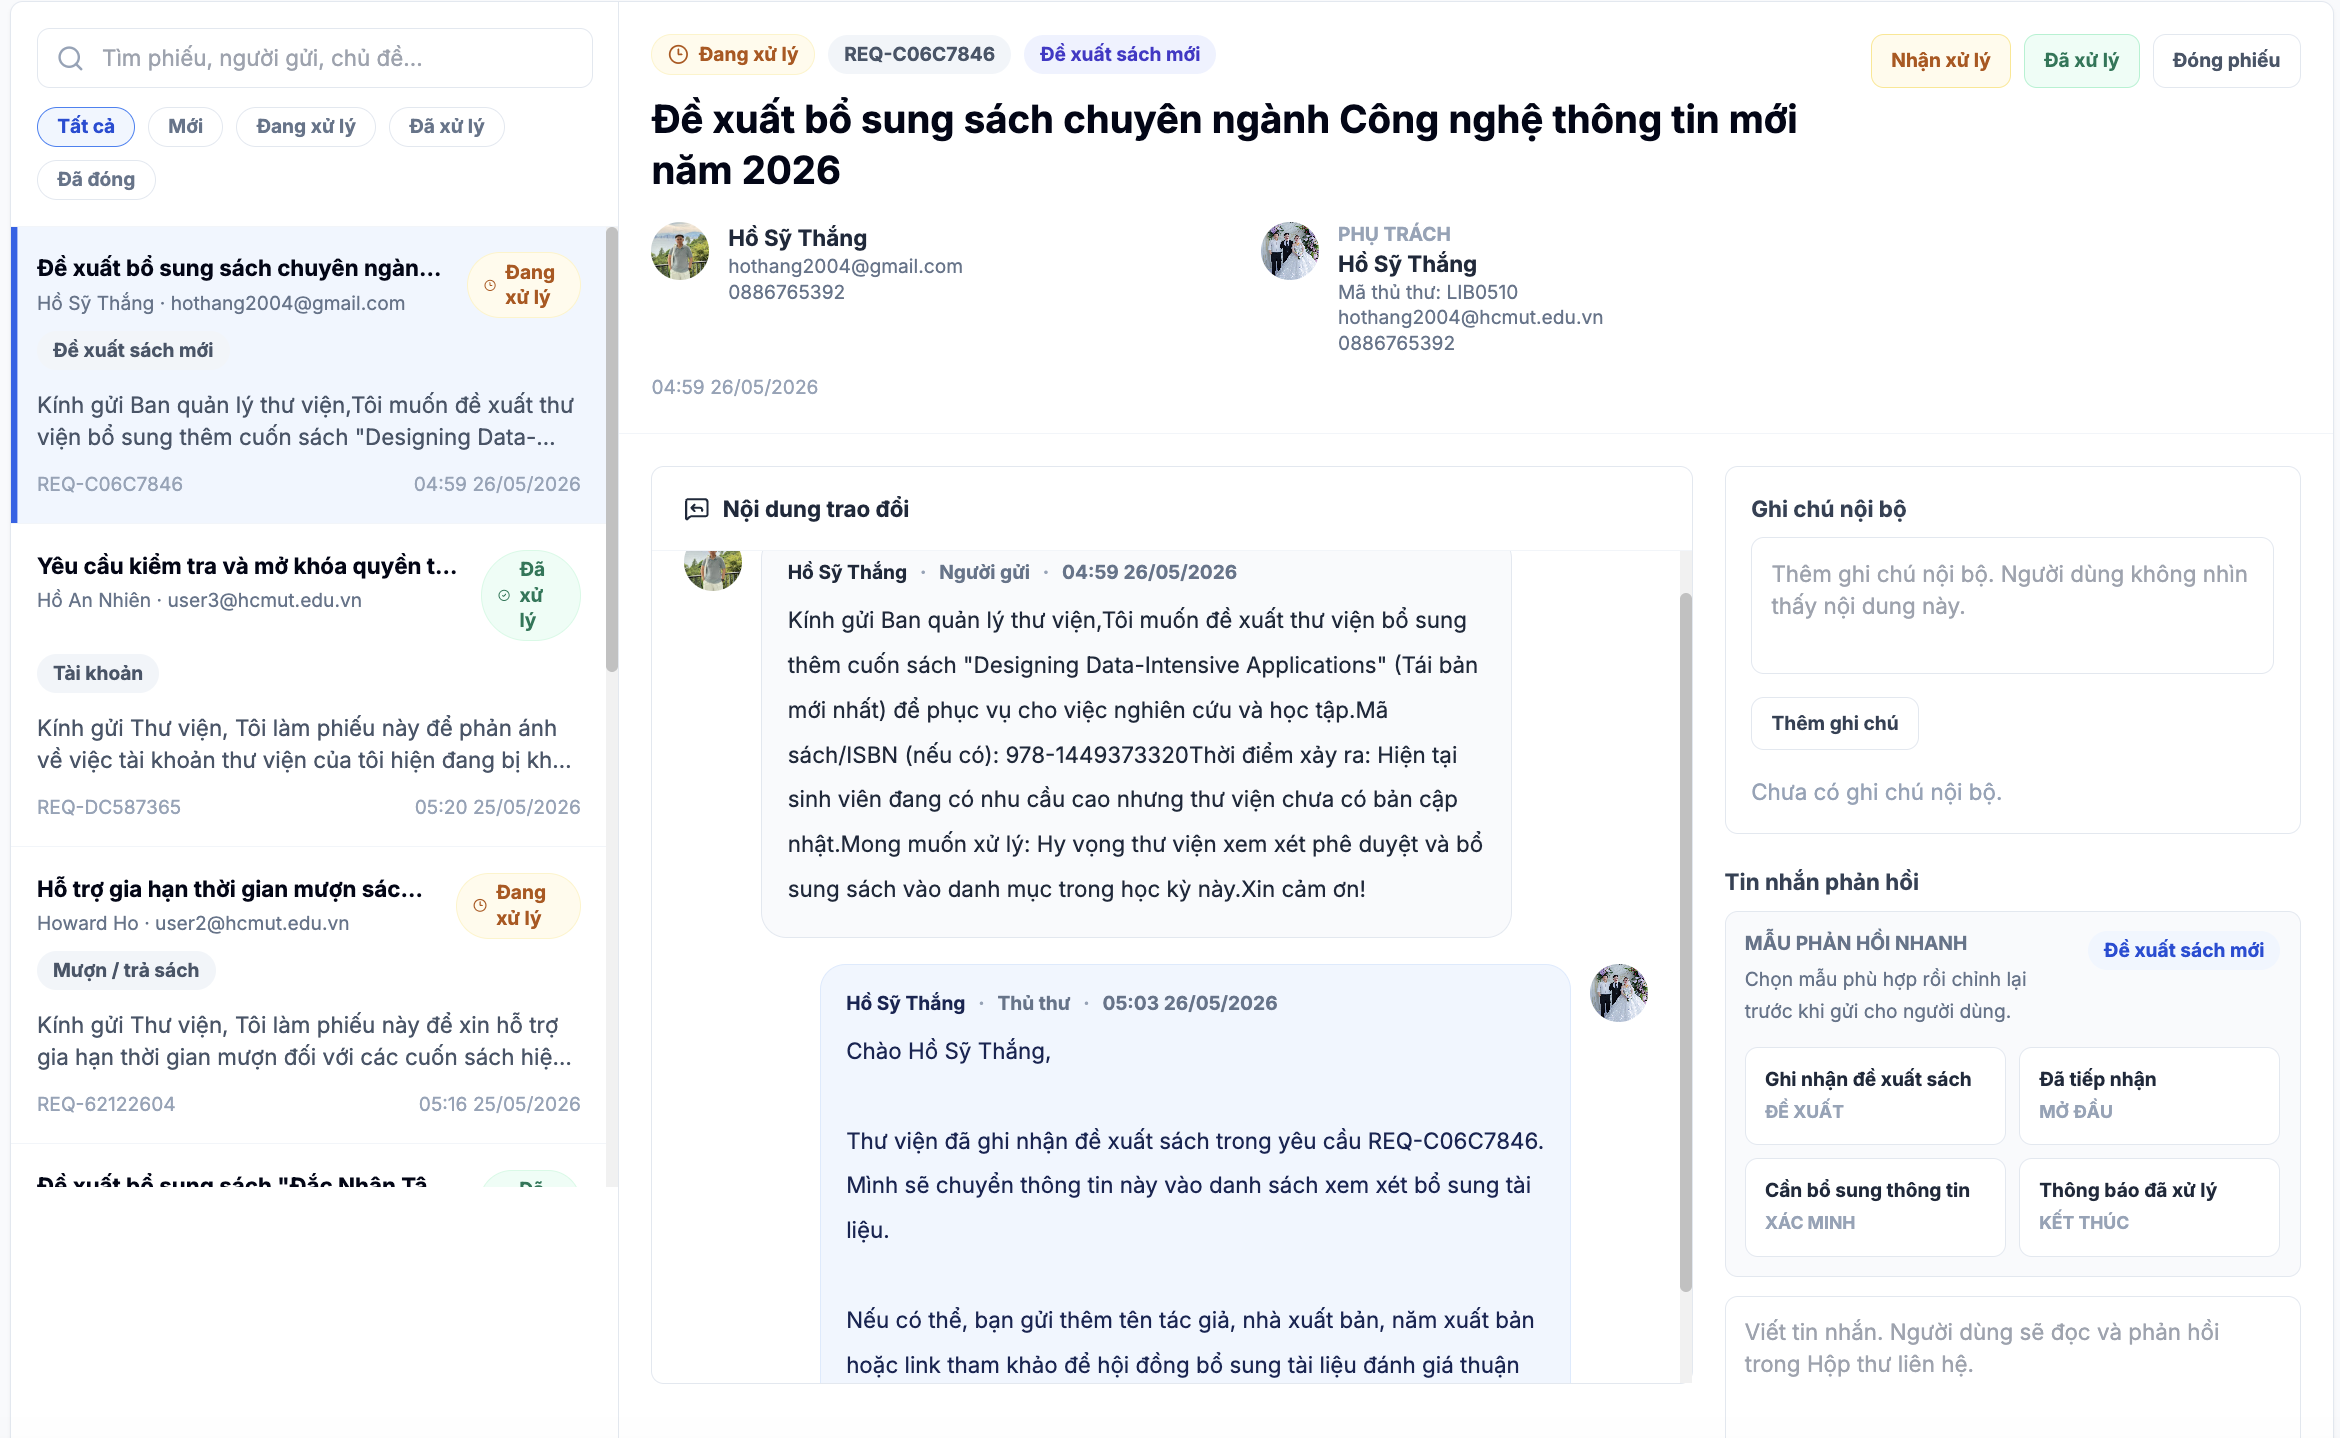
\includegraphics[width=\linewidth]{figures/ch06/frontend/contact_and_support_librarian.png}
        \caption{Tiếp nhận và phản hồi (Thủ thư)}
    \end{subfigure}
    \caption{Luồng giao tiếp và hỗ trợ trực tuyến giữa các nhóm người dùng}
    \label{fig:fe_cross_support}
\end{figure}

\begin{figure}[H]
    \centering
    \begin{subfigure}[b]{0.48\textwidth}
        \centering
        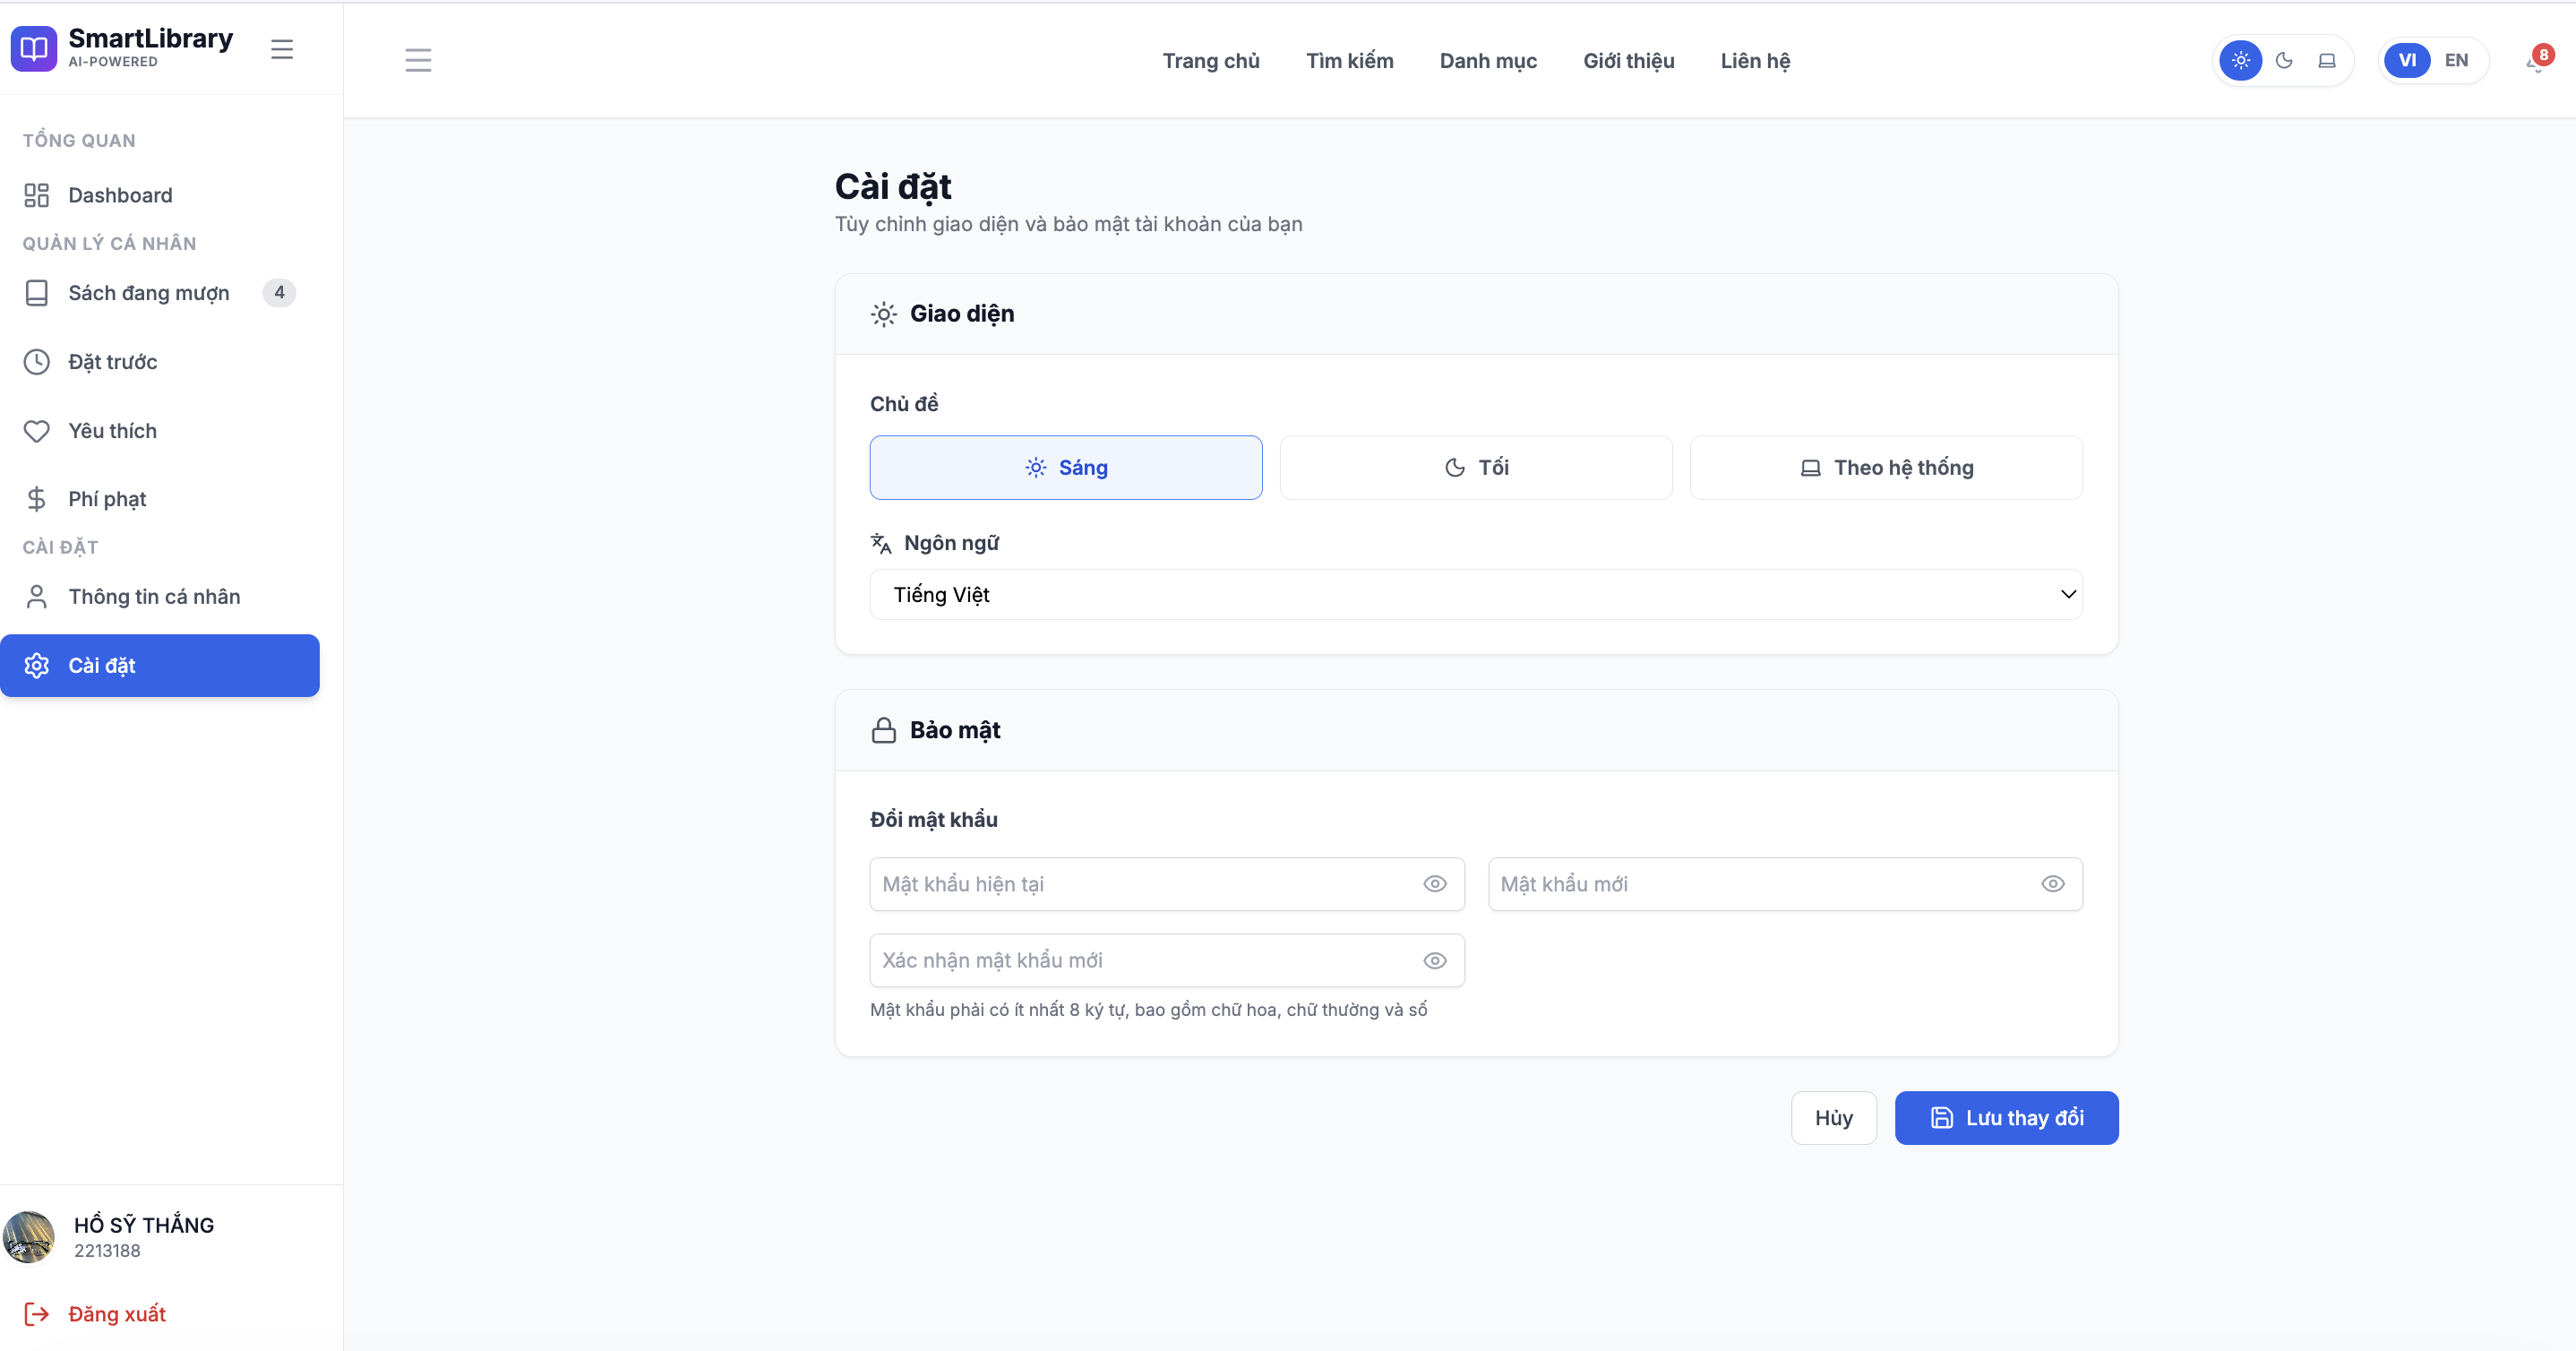
\includegraphics[width=\linewidth]{figures/ch06/frontend/light_theme_and_vietnamese.png}
        \caption{Giao diện sáng (Light) - Tiếng Việt}
    \end{subfigure}
    \hfill
    \begin{subfigure}[b]{0.48\textwidth}
        \centering
        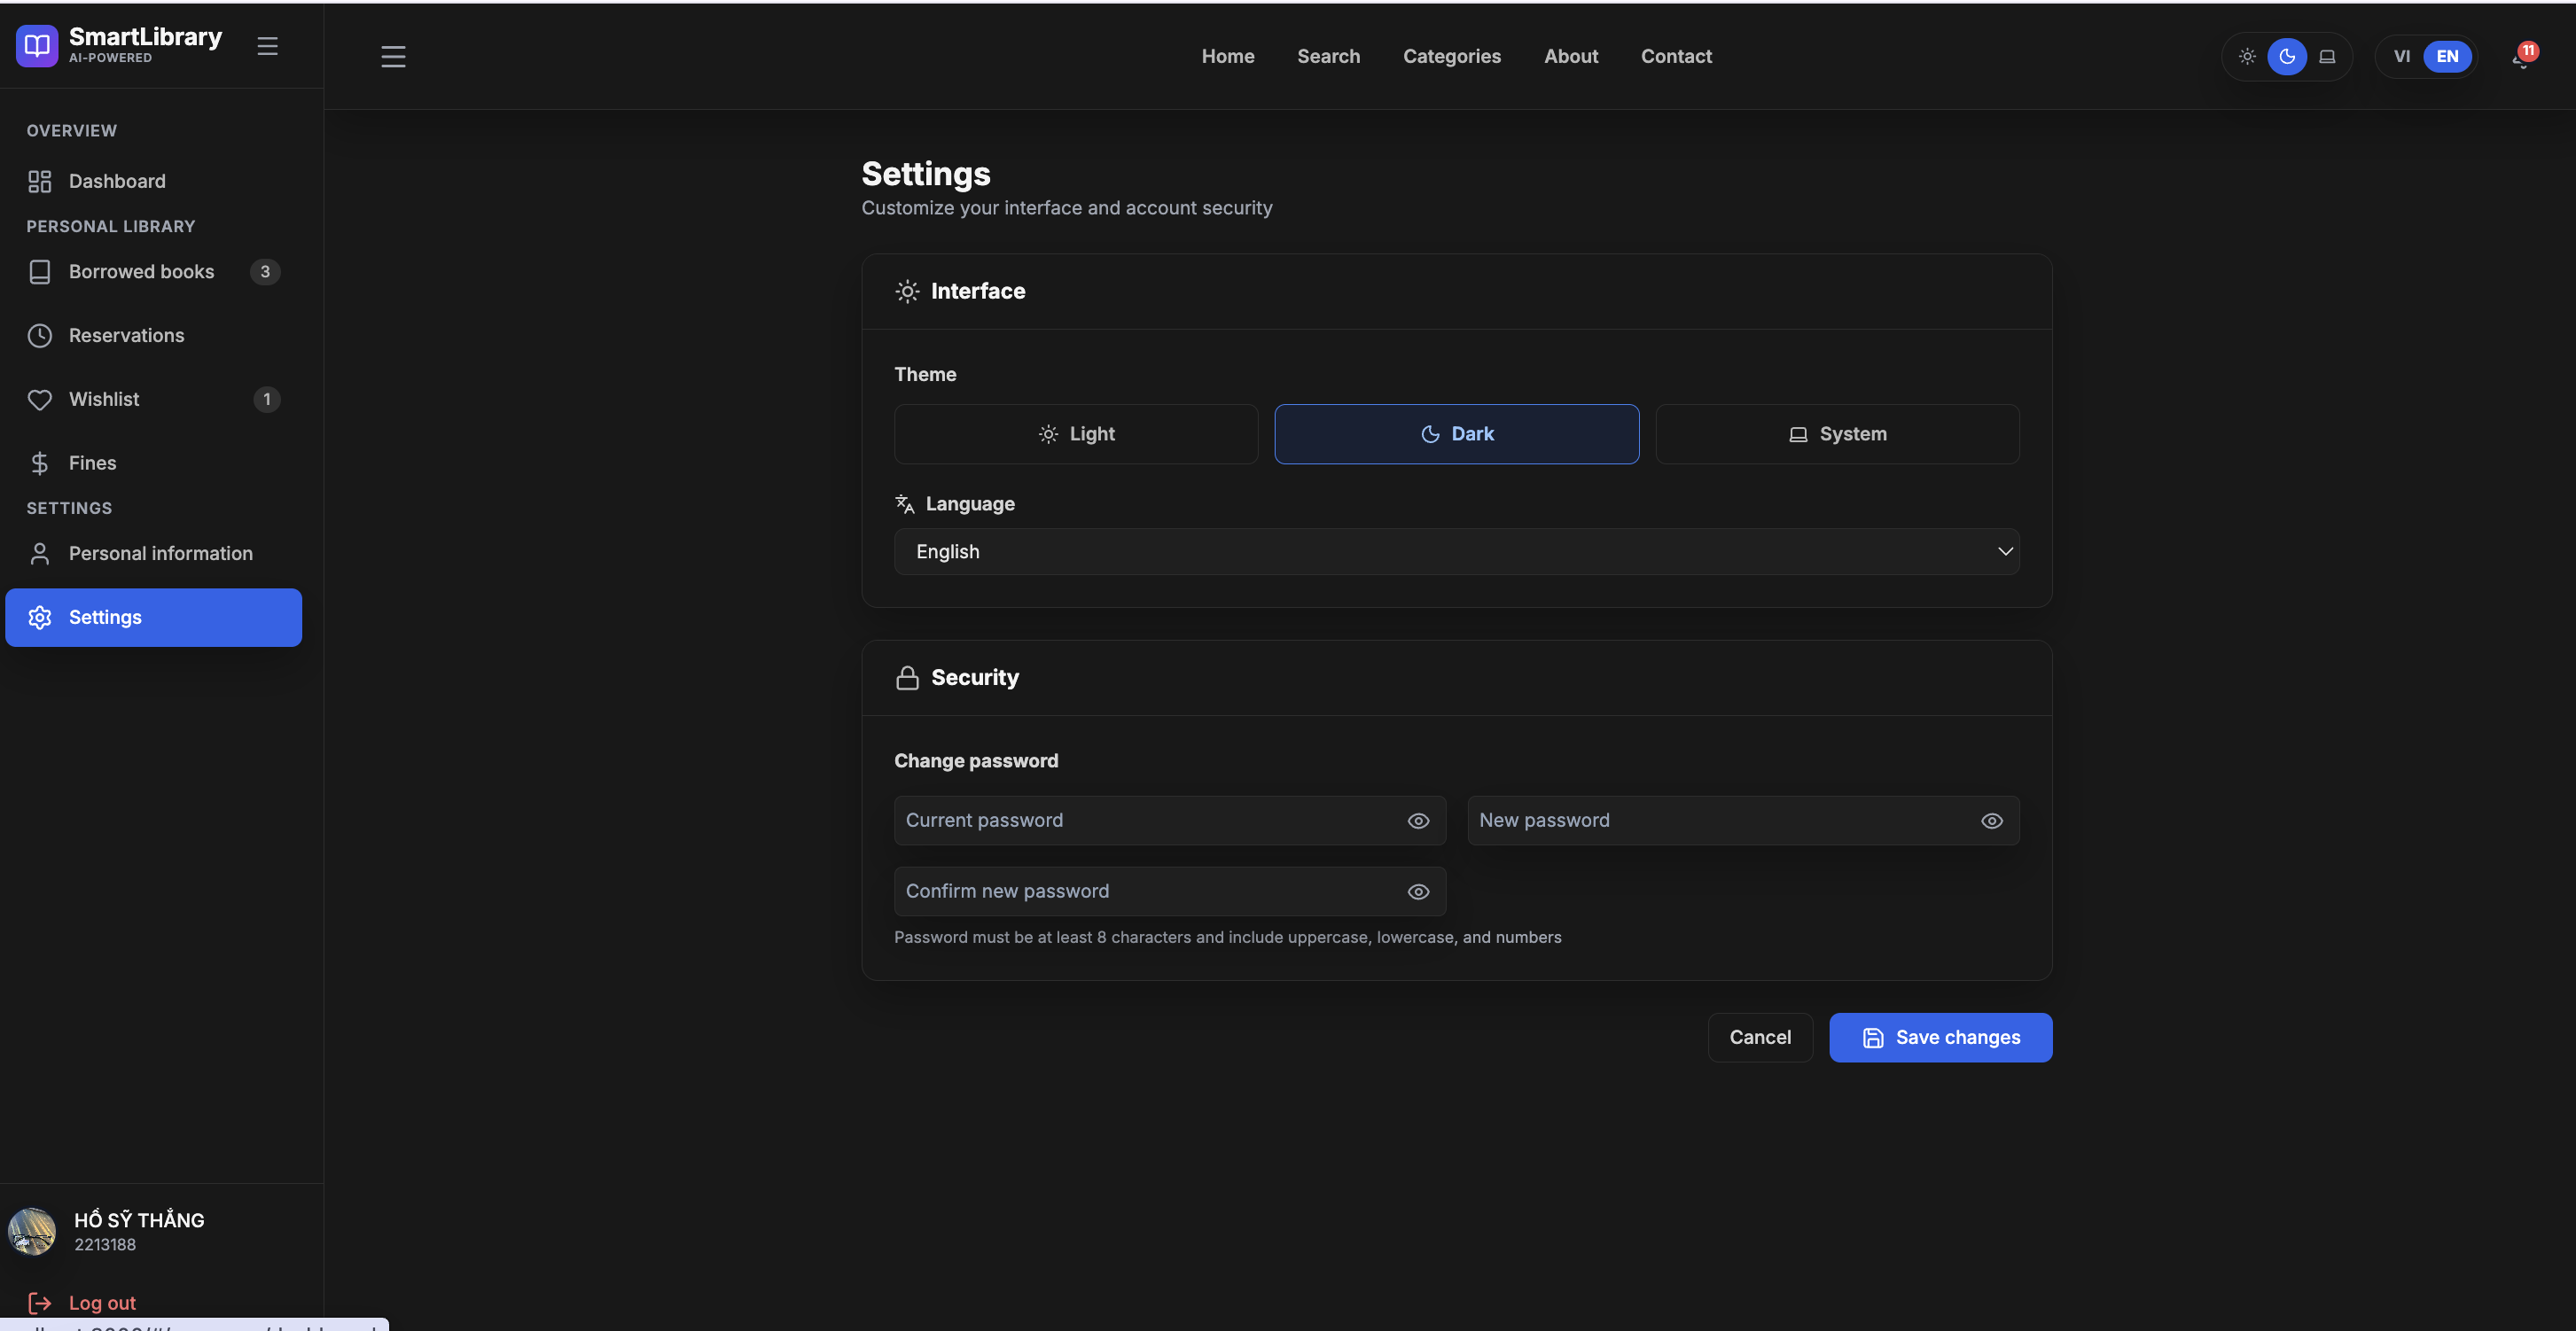
\includegraphics[width=\linewidth]{figures/ch06/frontend/dark_theme_and_english.png}
        \caption{Giao diện tối (Dark) - Tiếng Anh}
    \end{subfigure}
    \caption{Tính năng cá nhân hóa giao diện và đa ngôn ngữ (i18n)}
    \label{fig:fe_system_personalization}
\end{figure}

% --- ĐOẠN CHUYỂN Ý 1: TỪ GIAO DIỆN SANG KỸ THUẬT ---
Đằng sau giao diện trực quan và các trải nghiệm cá nhân hóa linh hoạt, phân hệ Frontend được xây dựng dựa trên một kiến trúc kỹ thuật vững chắc nhằm đảm bảo tính mở rộng và hiệu năng cao. Bảng \ref{tab:fe_technical_summary} tổng hợp các giải pháp kỹ thuật trọng tâm đã được áp dụng để giải quyết các bài toán cốt lõi: từ quản lý trạng thái tập trung, tối ưu giao tiếp API, đến xử lý luồng sự kiện thời gian thực (real-time) và tích hợp an toàn các dịch vụ bên thứ ba.

\begin{table}[H]
\centering
\small
\begin{tabularx}{\textwidth}{|p{3.4cm}|X|}
\hline
\textbf{Hạng mục Frontend} & \textbf{Nội dung đã hiện thực} \\
\hline
Routing và phân quyền &
\texttt{HashRouter}, lazy loading theo page, \texttt{ProtectedRoute}, redirect
theo role \texttt{student}, \texttt{librarian}, \texttt{admin}. \\
\hline
State dùng chung &
\texttt{AuthContext}, \texttt{LanguageContext}, \texttt{ThemeContext},
\texttt{NotificationContext}, \texttt{UploadContext}, \texttt{AppDialogContext}. \\
\hline
Giao tiếp API &
Axios instance, gắn JWT và \texttt{Accept-Language}, unwrap response, xử lý lỗi
nghiệp vụ, refresh token bằng queue để tránh gọi refresh nhiều lần. \\
\hline
Realtime và notification &
STOMP/SockJS, unread count, toast realtime, đánh dấu đã đọc và đồng bộ danh sách
thông báo. \\
\hline
Upload và tài liệu &
Upload bìa/PDF bằng presigned URL, hiển thị progress, cảnh báo khi đóng tab lúc
upload đang chạy, gửi yêu cầu AI xử lý tài liệu. \\
\hline
Thanh toán &
Khởi tạo thanh toán PayOS, hiển thị QR, polling trạng thái, cập nhật UI cho thủ
thư và bạn đọc sau khi thanh toán. \\
\hline
Cá nhân hóa &
Light/dark/system theme, song ngữ Việt--Anh, lưu cấu hình vào
\texttt{localStorage}, cập nhật \texttt{document.lang}. \\
\hline
\end{tabularx}
\caption{Các hạng mục kỹ thuật Frontend}
\label{tab:fe_technical_summary}
\end{table}

% --- ĐOẠN CHUYỂN Ý 2: TỪ KỸ THUẬT SANG GIÁ TRỊ THỰC TIỄN ---
Tất cả các quyết định về mặt kiến trúc và kỹ thuật nêu trên đều hướng tới một mục tiêu duy nhất: chuyển hóa công nghệ thành giá trị sử dụng. Bảng \ref{tab:fe_value_highlights} đúc kết lại những điểm sáng nổi bật của phân hệ, minh chứng cho việc ứng dụng công nghệ không chỉ dừng lại ở mặt hiển thị mà đã thực sự giải quyết triệt để các bài toán vận hành, chuyển đổi toàn diện trải nghiệm của bạn đọc và thủ thư.

\begin{table}[H]
\centering
\small
\begin{tabularx}{\textwidth}{|p{3.4cm}|X|p{3.4cm}|}
\hline
\textbf{Giá trị hiện thực} & \textbf{Cách hệ thống đã làm} & \textbf{Tác động với người dùng} \\
\hline
Tìm kiếm đa hướng &
Kết hợp keyword search, bộ lọc catalog, tag/category alias và semantic search. &
Bạn đọc không cần nhớ chính xác tên sách vẫn có thể tìm tài liệu phù hợp. \\
\hline
Vận hành tại quầy &
Màn hình thủ thư hỗ trợ mượn trực tiếp, xác nhận nhận sách, trả sách, ghi chú và xử lý phí. &
Nghiệp vụ mượn--trả không còn chỉ nằm ở phần demo giao diện. \\
\hline
Tài liệu số &
Upload bìa/PDF, progress upload, presigned URL và kích hoạt AI xử lý nền. &
Thủ thư có thể đưa tài liệu mới vào hệ thống và theo dõi kết quả xử lý. \\
\hline
Phản hồi tức thời &
Toast, notification realtime, unread count và đồng bộ trạng thái thanh toán/đặt trước. &
Người dùng biết ngay khi có thay đổi quan trọng thay vì phải tải lại trang. \\
\hline
\end{tabularx}
\caption{Các điểm giá trị nổi bật ở Frontend}
\label{tab:fe_value_highlights}
\end{table}

\subsection{Hiện thực Backend}

Nhóm đã hiện thực backend bằng Spring Boot 3.3.5 và Java 21 theo mô hình modular
monolith. Backend là lớp kiểm soát chính của hệ thống: xác thực, phân quyền,
giao dịch mượn--trả, trạng thái bản sao, phí phạt, thanh toán, thông báo, audit
và gateway sang AI service đều đi qua backend. Cấu trúc module được chia theo
miền nghiệp vụ để dễ bảo trì nhưng vẫn triển khai trong một ứng dụng thống nhất.


Để hiện thực hóa tư tưởng thiết kế này, hệ thống được phân rã thành các miền nghiệp vụ độc lập (Bounded Contexts) nhưng vẫn chia sẻ chung một lõi nền tảng (\texttt{library-shared}). Hình \ref{fig:be_architecture_diagram} minh họa chi tiết sơ đồ kiến trúc tổng thể của hệ thống. Trong đó, các module giao tiếp với nhau thông qua cơ chế hướng sự kiện (Event-driven) bằng Apache Kafka hoặc qua các giao diện hợp đồng, giúp giảm thiểu tối đa sự phụ thuộc chéo (tight-coupling).

\begin{figure}[H]
    \centering
    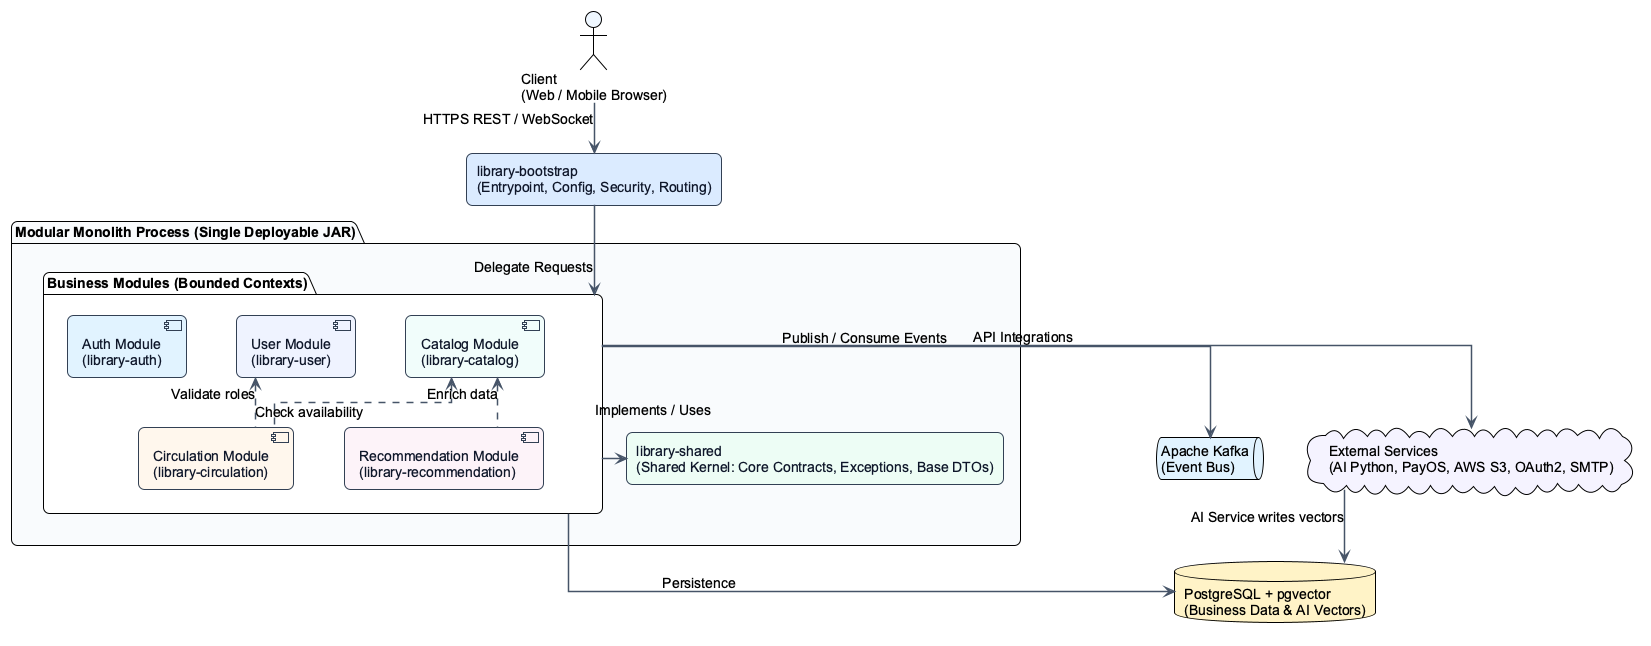
\includegraphics[width=\textwidth]{figures/ch06/backend/backend_architecture.png}
    \caption{Sơ đồ kiến trúc Modular Monolith tổng thể}
    \label{fig:be_architecture_diagram}
\end{figure}

Tương ứng với sơ đồ kiến trúc, mã nguồn vật lý cũng được tổ chức phân rã một cách chặt chẽ. Hình \ref{fig:be_folder_structure} thể hiện cấu trúc thư mục thực tế của dự án, minh chứng cho việc áp dụng triệt để mô hình Modular Monolith vào khâu triển khai mã nguồn.

\begin{figure}[H]
    \centering
    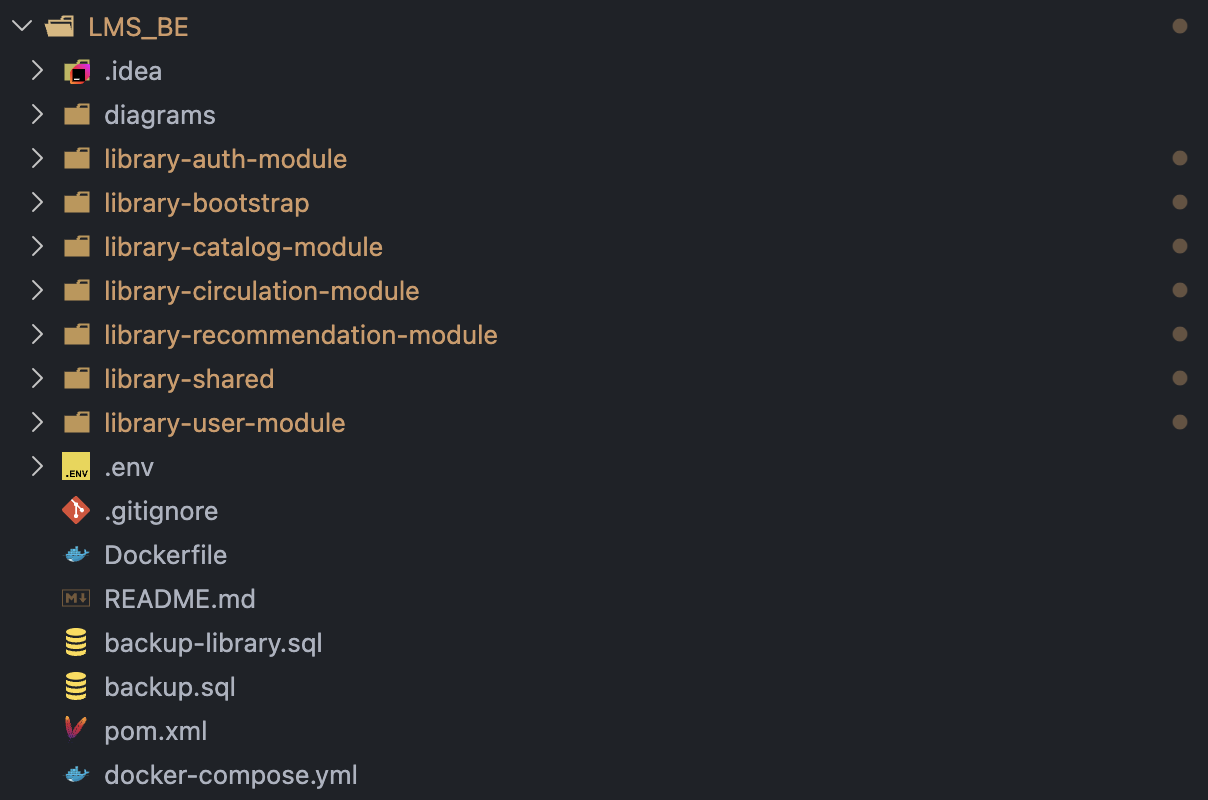
\includegraphics[width=0.45\textwidth]{figures/ch06/backend/backend_folder_tree.png}
    \caption{Cấu trúc thư mục mã nguồn Backend thực tế}
    \label{fig:be_folder_structure}
\end{figure}

Nhờ cấu trúc phân mảnh rõ ràng, toàn bộ các điểm cuối giao tiếp (API endpoints) của hệ thống đều được quy chuẩn hóa và tự động sinh tài liệu thông qua OpenAPI/Swagger. Do quy mô hệ thống lớn với hàng trăm API, Hình \ref{fig:be_swagger_publication} trích xuất giao diện API của module đại diện (Publication Controller) nhằm minh chứng cho mức độ chi tiết và tính chuẩn mực của các API Contract, đảm bảo sự minh bạch khi tích hợp với Frontend và AI Service.

\begin{figure}[H]
    \centering
    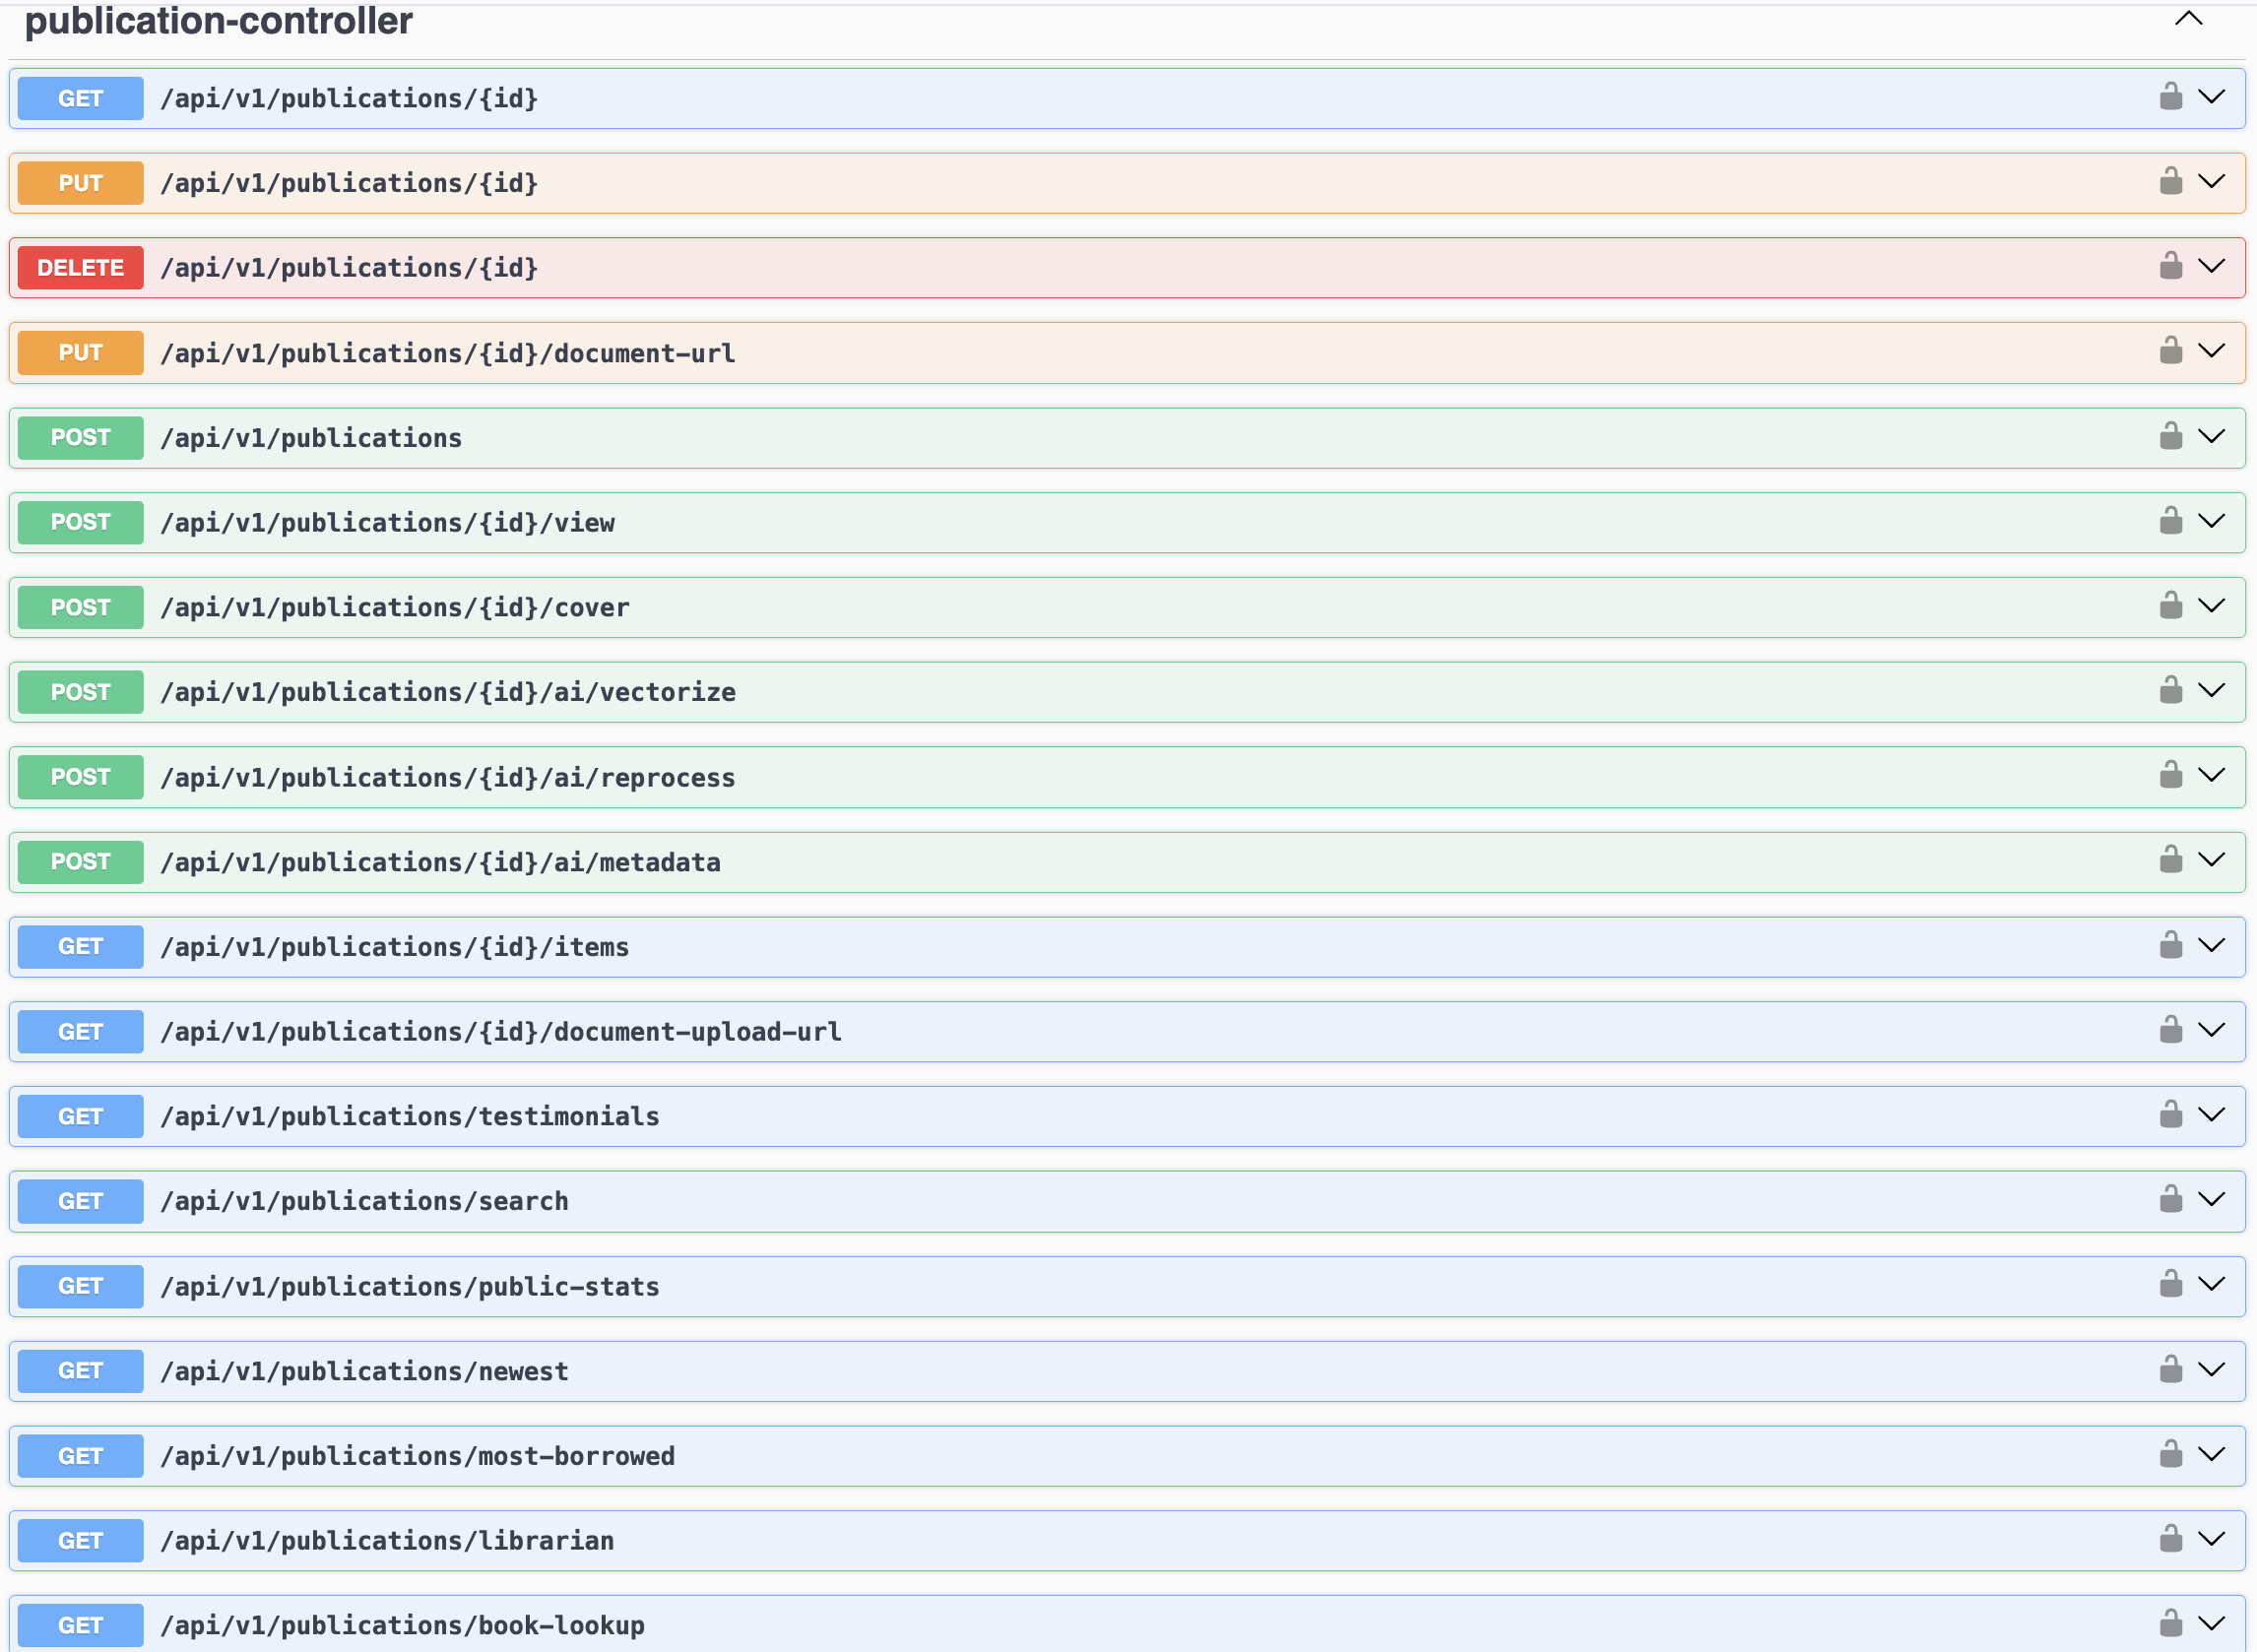
\includegraphics[width=0.85\linewidth]{figures/ch06/backend/publication-controller-swagger.png}
    \caption{Tài liệu hóa API tự động bằng Swagger (Đại diện module Publication)}
    \label{fig:be_swagger_publication}
\end{figure}

Chi tiết nhiệm vụ và nội dung hiện thực của toàn bộ các phân hệ con trong kiến trúc Backend được tổng hợp cụ thể tại Bảng \ref{tab:be_modules_implemented}.

% (Giữ nguyên Bảng \begin{longtable} của bạn ở bên dưới)

\begin{longtable}{|p{3.8cm}|p{4cm}|p{6.5cm}|}
\caption{Các module Backend đã hiện thực}
\label{tab:be_modules_implemented}\\
\hline
\textbf{Module} & \textbf{Nhóm chức năng} & \textbf{Nội dung đã hiện thực} \\
\hline
\endfirsthead
\hline
\textbf{Module} & \textbf{Nhóm chức năng} & \textbf{Nội dung đã hiện thực} \\
\hline
\endhead
\texttt{library-bootstrap} & Khởi động hệ thống &
Cấu hình Spring Boot, datasource, JPA, Flyway, Kafka, mail, OpenAPI, async,
security, CORS và biến môi trường triển khai. \\
\hline
\texttt{library-shared} & Thành phần dùng chung &
Response wrapper, exception, error code, base entity, DTO dùng chung, shared
port, Kafka event, S3 storage port và audit logging aspect. \\
\hline
\texttt{library-auth-module} & Xác thực &
Đăng ký, đăng nhập, refresh token, logout, xác thực email, quên mật khẩu, đặt
lại mật khẩu, Google OAuth2, JWT decoder và WebSocket authentication. \\
\hline
\texttt{library-user-module} & Người dùng và thông báo &
Hồ sơ người dùng, avatar, đổi mật khẩu, vai trò, trạng thái tài khoản, danh sách
notification, Kafka consumer và WebSocket push. \\
\hline
\texttt{library-admin-module} & Quản trị &
Quản lý tài khoản độc giả/thủ thư, tạo thủ thư, khóa/mở khóa, xác minh tài
khoản, cấu hình chính sách mượn trả và audit log. \\
\hline
\texttt{library-catalog-module} & Catalog thư viện &
Ấn phẩm, bản sao, tác giả, nhà xuất bản, danh mục, tag, tìm kiếm công khai,
chi tiết sách, trạng thái bản sao, upload bìa và presigned URL cho PDF. \\
\hline
\texttt{library-circulation-module} & Mượn--trả &
Yêu cầu mượn, mượn trực tiếp, xác nhận nhận sách, trả sách, đặt trước, hàng chờ,
gia hạn trạng thái, báo hư/mất và cập nhật trạng thái bản sao. \\
\hline
\texttt{library-circulation-module} & Phí phạt và scheduler &
Tính phí quá hạn/hư/mất, thanh toán tiền mặt, PayOS, nhắc sắp đến hạn, xử lý quá
hạn, hủy đặt trước hết hạn và dashboard vận hành. \\
\hline
\texttt{library-recommendation-module} & Tương tác bạn đọc &
Wishlist, lịch sử tìm kiếm, lượt xem, rating, comment, phản hồi rating của thủ
thư, đánh giá hệ thống và thống kê tương tác. \\
\hline
\texttt{library-recommendation-module} & AI Gateway &
Gọi semantic search, sách tương tự, recommendation, gửi yêu cầu xử lý PDF, nhận
AI callback có HMAC và cập nhật metadata AI về publication. \\
\hline
\end{longtable}

Để đảm bảo các miền nghiệp vụ nêu trên phối hợp nhịp nhàng và chịu tải tốt, toàn bộ hệ thống được xây dựng trên một bộ tiêu chuẩn kỹ thuật cốt lõi nghiêm ngặt. Bảng \ref{tab:be_technical_summary} trình bày chi tiết các giải pháp nền tảng đã được triển khai, bao gồm chuẩn hóa giao tiếp API, cơ chế bảo mật không trạng thái (stateless), quản trị cơ sở dữ liệu tập trung và các luồng xử lý tác vụ nền bất đồng bộ.

\begin{table}[H]
\centering
\small
\begin{tabularx}{\textwidth}{|p{3.6cm}|X|}
\hline
\textbf{Hạng mục Backend} & \textbf{Nội dung đã hiện thực} \\
\hline
Chuẩn API &
\texttt{ApiResponseApp}, \texttt{PageResponse}, mã lỗi nghiệp vụ, message theo
\texttt{Accept-Language}, \texttt{GlobalExceptionHandler}. \\
\hline
Bảo mật &
Spring Security stateless, JWT, refresh token, Google OAuth2, kiểm tra role bằng
annotation và AOP, khóa tài khoản có hiệu lực ngay khi đăng nhập. \\
\hline
Dữ liệu &
PostgreSQL, Flyway migration, entity audit, phân biệt ấn phẩm và bản sao, lưu
trạng thái giao dịch, fine, reservation, notification và dữ liệu AI. \\
\hline
Tác vụ nền &
Scheduler nhắc hạn, xử lý quá hạn, hủy reservation hết hạn, Kafka event cho
notification và async callback sang frontend. \\
\hline
Tích hợp ngoài &
S3-compatible storage, email SMTP, Google OAuth2, PayOS, AI service, WebSocket
và Swagger/OpenAPI. \\
\hline
Quan sát vận hành &
Audit log, dashboard thủ thư, dashboard admin, lỗi nghiệp vụ có mã rõ ràng và
log cho callback/tác vụ nền. \\
\hline
\end{tabularx}
\caption{Các hạng mục kỹ thuật Backend}
\label{tab:be_technical_summary}
\end{table}

% --- ĐOẠN CHUYỂN Ý 2: TỪ KỸ THUẬT SANG GIÁ TRỊ VẬN HÀNH ---
Việc áp dụng kiến trúc Modular Monolith và các công nghệ phụ trợ không chỉ nhằm mục đích đáp ứng yêu cầu phần mềm, mà còn trực tiếp giải quyết các bài toán vận hành thực tế của một thư viện hiện đại. Bảng \ref{tab:be_value_highlights} đúc kết những giá trị cốt lõi mà thiết kế Backend đã mang lại, từ việc đảm bảo tính toàn vẹn dữ liệu xuyên suốt các giao dịch mượn trả, khả năng bảo trì hệ thống, cho đến độ an toàn tuyệt đối khi giao tiếp với các dịch vụ bên ngoài (External Services).

\begin{table}[H]
\centering
\small
\begin{tabularx}{\textwidth}{|p{3.4cm}|X|p{3.4cm}|}
\hline
\textbf{Điểm hiện thực} & \textbf{Nội dung đã làm} & \textbf{Ý nghĩa vận hành} \\
\hline
Ranh giới module &
Auth, user, admin, catalog, circulation và recommendation tách theo miền nghiệp vụ. &
Dễ đọc code, dễ kiểm thử và giảm phụ thuộc chéo khi mở rộng. \\
\hline
Luồng trạng thái sách &
Backend kiểm soát item, transaction, reservation, fine và notification theo một nguồn dữ liệu thống nhất. &
Tránh lệch trạng thái giữa giao diện bạn đọc và giao diện thủ thư. \\
\hline
Tích hợp ngoài &
PayOS, Google OAuth2, email, storage, AI service, WebSocket và Swagger/OpenAPI. &
Hệ thống có khả năng chạy như một sản phẩm hoàn chỉnh, không chỉ là prototype. \\
\hline
An toàn callback &
Webhook PayOS và callback AI đều có cơ chế kiểm tra chữ ký hoặc token. &
Giảm rủi ro cập nhật trạng thái giả từ request bên ngoài. \\
\hline
\end{tabularx}
\caption{Các điểm giá trị nổi bật ở Backend}
\label{tab:be_value_highlights}
\end{table}

\subsection{Hiện thực AI Service}

AI service được tách thành một tiến trình Python riêng để xử lý các tác vụ có
đặc thù tính toán và phụ thuộc mô hình. Service này không quyết định nghiệp vụ
mượn--trả; nó chỉ sinh metadata, vector, điểm tương đồng hoặc danh sách mã ấn
phẩm. Backend luôn là nơi chuẩn hóa kết quả cuối cùng trước khi trả về frontend.

Để đáp ứng được đặc thù xử lý này, kiến trúc nội bộ của AI Service được phân tách thành luồng xử lý đồng bộ (Synchronous Gateway) và luồng xử lý nền bất đồng bộ (Background Worker). Hình \ref{fig:ai_architecture} mô tả bức tranh tổng thể về cách AI Service tương tác với các thành phần trong hệ thống: từ việc nhận yêu cầu từ Spring Boot, tải tài liệu vật lý từ AWS S3, cho đến việc giao tiếp với LLM (Google Gemini) để trích xuất tri thức. Đặc biệt, để đảm bảo tính toàn vẹn dữ liệu, mọi bản cập nhật trạng thái từ tiến trình xử lý nền (Worker) trả về Backend đều được ký xác thực bằng thuật toán mã hóa HMAC (Hash-based Message Authentication Code).

\begin{figure}[H]
    \centering
    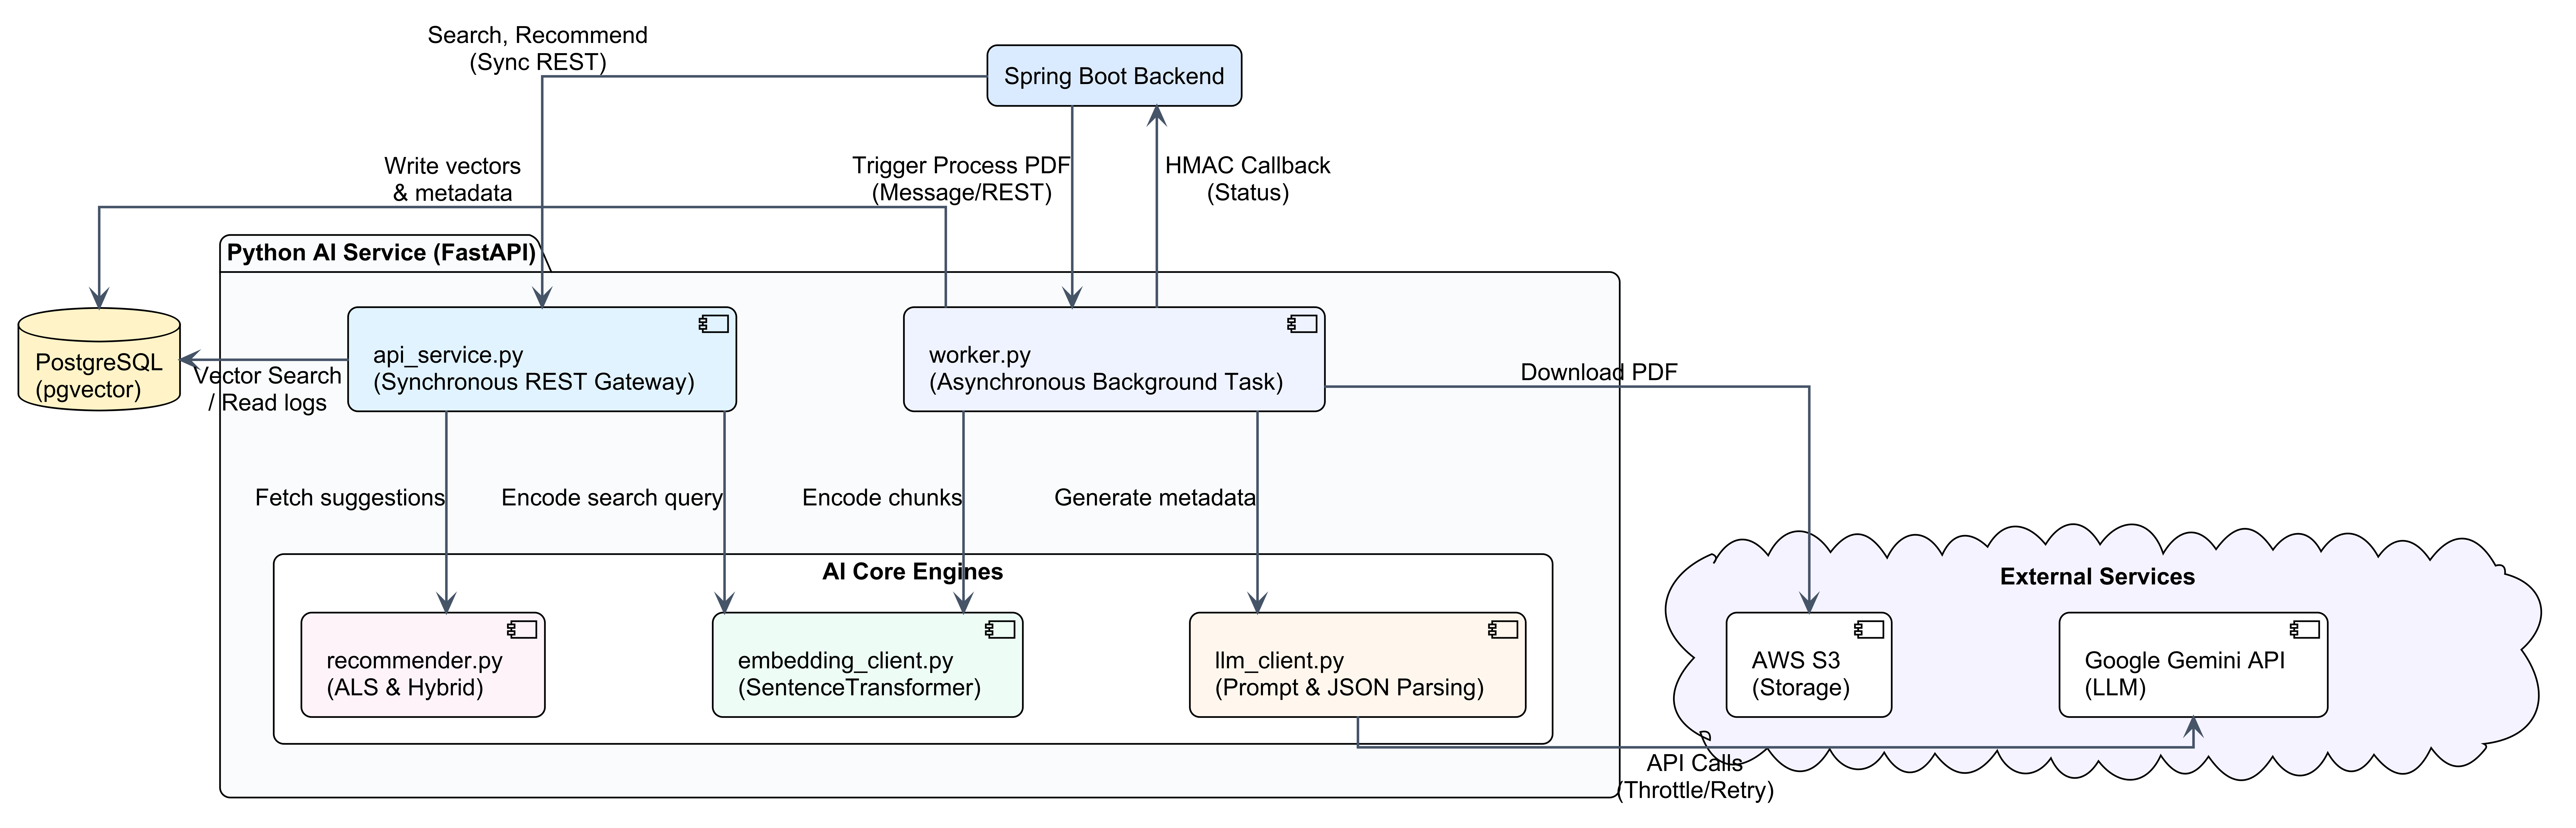
\includegraphics[width=\textwidth]{figures/ch06/ai/ai_architecture.png}
    \caption{Kiến trúc tổng thể và luồng giao tiếp của AI Service}
    \label{fig:ai_architecture}
\end{figure}

Lõi sức mạnh của phân hệ AI nằm ở luồng xử lý và số hóa tài liệu (ETL Pipeline). Khi một tài liệu PDF mới được hệ thống ghi nhận, tiến trình ETL (Hình \ref{fig:ai_etl_pipeline}) sẽ tự động được kích hoạt. Quá trình này trải qua nhiều công đoạn phức tạp: làm sạch nhiễu (Header/Footer), chia nhỏ văn bản bằng kỹ thuật Cửa sổ trượt (Sliding Window), sinh vector nhúng (Embedding) bằng mô hình SentenceTransformer tiếng Việt, và cuối cùng là đúc kết siêu dữ liệu (Tóm tắt, Phân loại độc giả, Gắn thẻ) thông qua LLM trước khi lưu trữ vào cơ sở dữ liệu \texttt{pgvector}.

\begin{figure}[H]
    \centering
    % Hạ tỷ lệ chiều rộng xuống để chiều cao tự động co ngắn lại vừa trang
    \includegraphics[width=0.52\textwidth]{figures/ch06/ai/ai_etl_pipeline.png}
    \caption{Luồng xử lý trích xuất, biến đổi và tải dữ liệu (ETL Pipeline) cho tài liệu PDF}
    \label{fig:ai_etl_pipeline}
\end{figure}

Chi tiết về chức năng và nhiệm vụ cụ thể của từng thành phần mã nguồn bên trong AI Service được thống kê tại Bảng \ref{tab:ai_components_implemented}.

% ================= NỐI TIẾP BẰNG BẢNG CỦA BẠN =================

\begin{longtable}{|p{3.8cm}|p{4cm}|p{6.5cm}|}
\caption{Các thành phần AI Service đã hiện thực}
\label{tab:ai_components_implemented}\\
\hline
\textbf{Thành phần} & \textbf{Nhóm chức năng} & \textbf{Nội dung đã hiện thực} \\
\hline
\endfirsthead
\hline
\textbf{Thành phần} & \textbf{Nhóm chức năng} & \textbf{Nội dung đã hiện thực} \\
\hline
\endhead
\texttt{api\_service.py} & FastAPI gateway &
Cung cấp health check, semantic search, similar publications, recommendation và
xử lý publication theo request đồng bộ. \\
\hline
\texttt{worker.py} & Xử lý nền &
Nhận message xử lý sách, tải PDF, chạy ETL, ghi trạng thái và gửi callback về
backend bằng chữ ký HMAC. \\
\hline
\texttt{pdf\_processing.py} & PDF ETL &
Tải/đọc PDF, trích xuất text bằng PyMuPDF, làm sạch header/footer/số trang, chia
chunk sliding window. \\
\hline
\texttt{pipeline.py} & Điều phối ETL &
Hash skip, sinh embedding, chọn chunk đại diện, reduce metadata bằng LLM, fallback
local khi lỗi và ghi kết quả vào database. \\
\hline
\texttt{embedding\_client.py} & Embedding &
Load SentenceTransformer tiếng Việt, sinh vector 768 chiều, normalize vector và
phục vụ semantic search/similar/recommendation. \\
\hline
\texttt{llm\_client.py} & Metadata AI &
Gọi Gemini, throttle/retry, ép output JSON, sinh summary, audience, tag tiếng
Việt và alias \texttt{tags\_en}. \\
\hline
\texttt{tag\_quality.py} & Làm sạch tag &
Lọc tag rác, chuẩn hóa alias Anh--Việt, map tag tiếng Việt sang thuật ngữ tiếng
Anh để hỗ trợ tìm kiếm song ngữ. \\
\hline
\texttt{recommender.py} & Gợi ý sách &
Huấn luyện ALS implicit feedback, kết hợp content-based, collaborative signal và
trending fallback. \\
\hline
\texttt{init\_schema.sql} & Dữ liệu AI &
Khởi tạo schema \texttt{ai\_engine}, bảng vector, ETL run, search log, index
pgvector và bảng recommendation. \\
\hline
\end{longtable}

% --- ĐOẠN CHUYỂN Ý 1: TỪ MODULE SANG MINH CHỨNG HÌNH ẢNH ---
Để minh chứng cho hoạt động của các thành phần mã nguồn nêu trên, hệ thống ghi nhận các kết quả đầu ra rõ rệt ở cả lớp giao diện người dùng lẫn lớp lưu trữ dữ liệu. Hình \ref{fig:ai_feature_showcase} thể hiện trải nghiệm trực quan của bạn đọc khi sử dụng công cụ tìm kiếm ngữ nghĩa và tiếp nhận các đề xuất sách cá nhân hóa. Song song đó, Hình \ref{fig:ai_etl_vector_showcase} cung cấp bằng chứng kỹ thuật (Technical Evidence) về tiến trình xử lý nền (ETL run) và cấu trúc dữ liệu vector nhiều chiều đã được lưu trữ thành công trong \texttt{pgvector}.

\begin{figure}[H]
    \centering
    \begin{subfigure}[b]{0.48\textwidth}
        \centering
        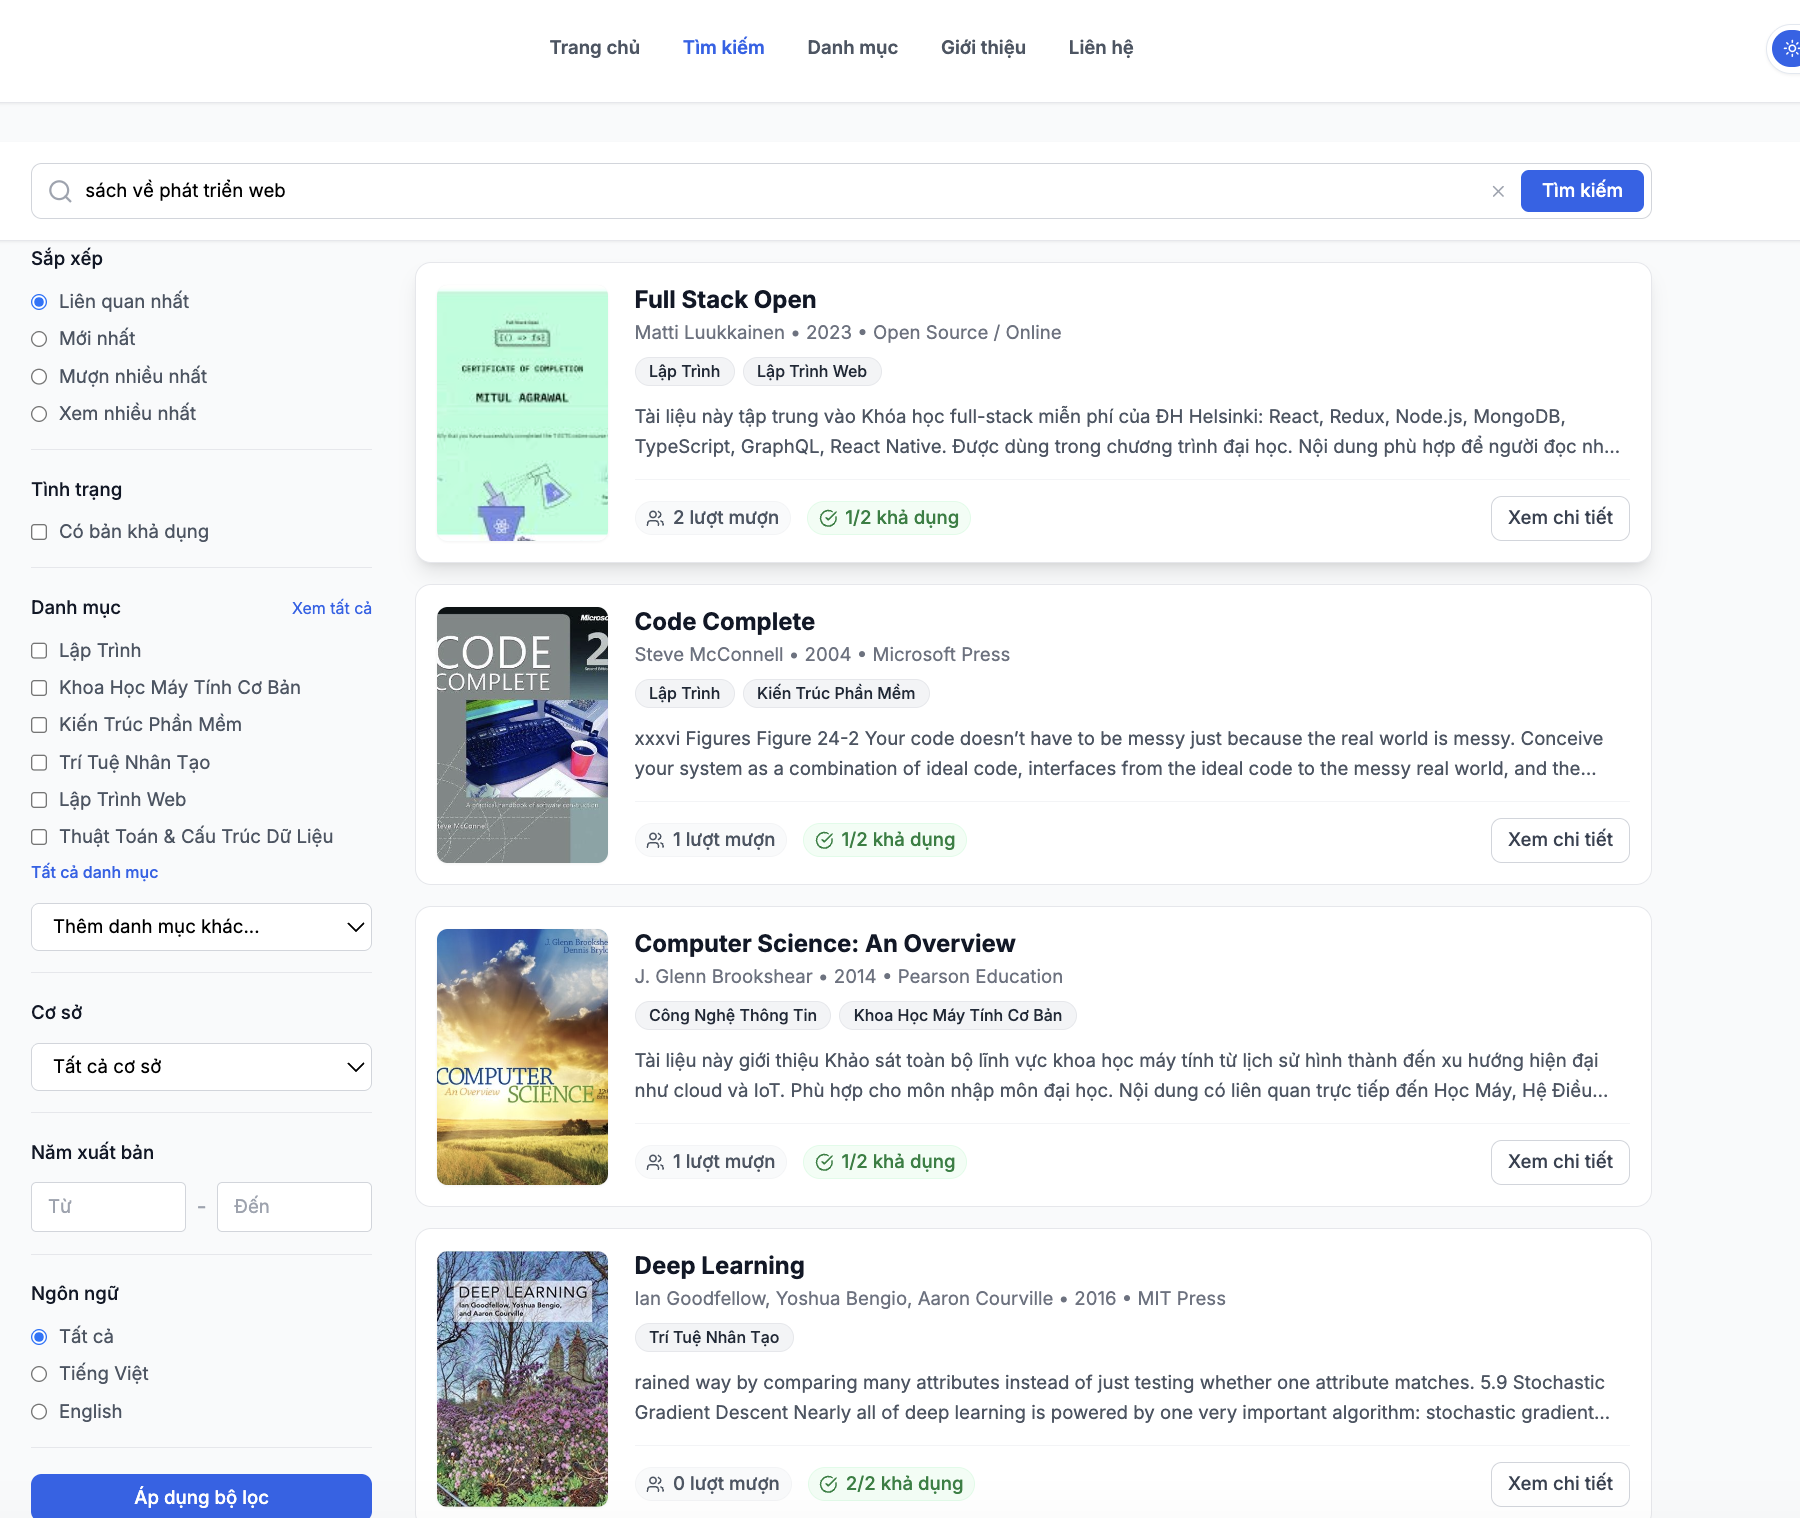
\includegraphics[width=\linewidth]{figures/ch06/ai/semantic_search.png}
        \caption{Semantic search}
    \end{subfigure}
    \hfill
    \begin{subfigure}[b]{0.48\textwidth}
        \centering
        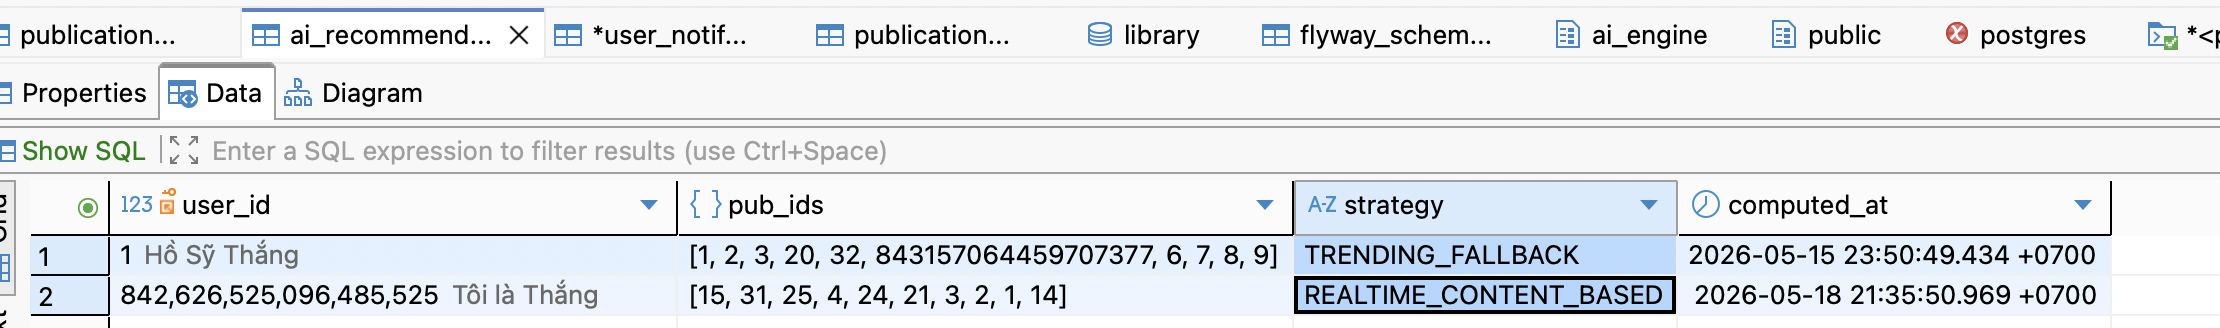
\includegraphics[width=\linewidth]{figures/ch06/ai/recommendation.png}
        \caption{Gợi ý sách}
    \end{subfigure}
    \caption{Các chức năng AI đã tích hợp vào hệ thống}
    \label{fig:ai_feature_showcase}
\end{figure}

\begin{figure}[H]
    \centering
    \begin{subfigure}[b]{0.48\textwidth}
        \centering
        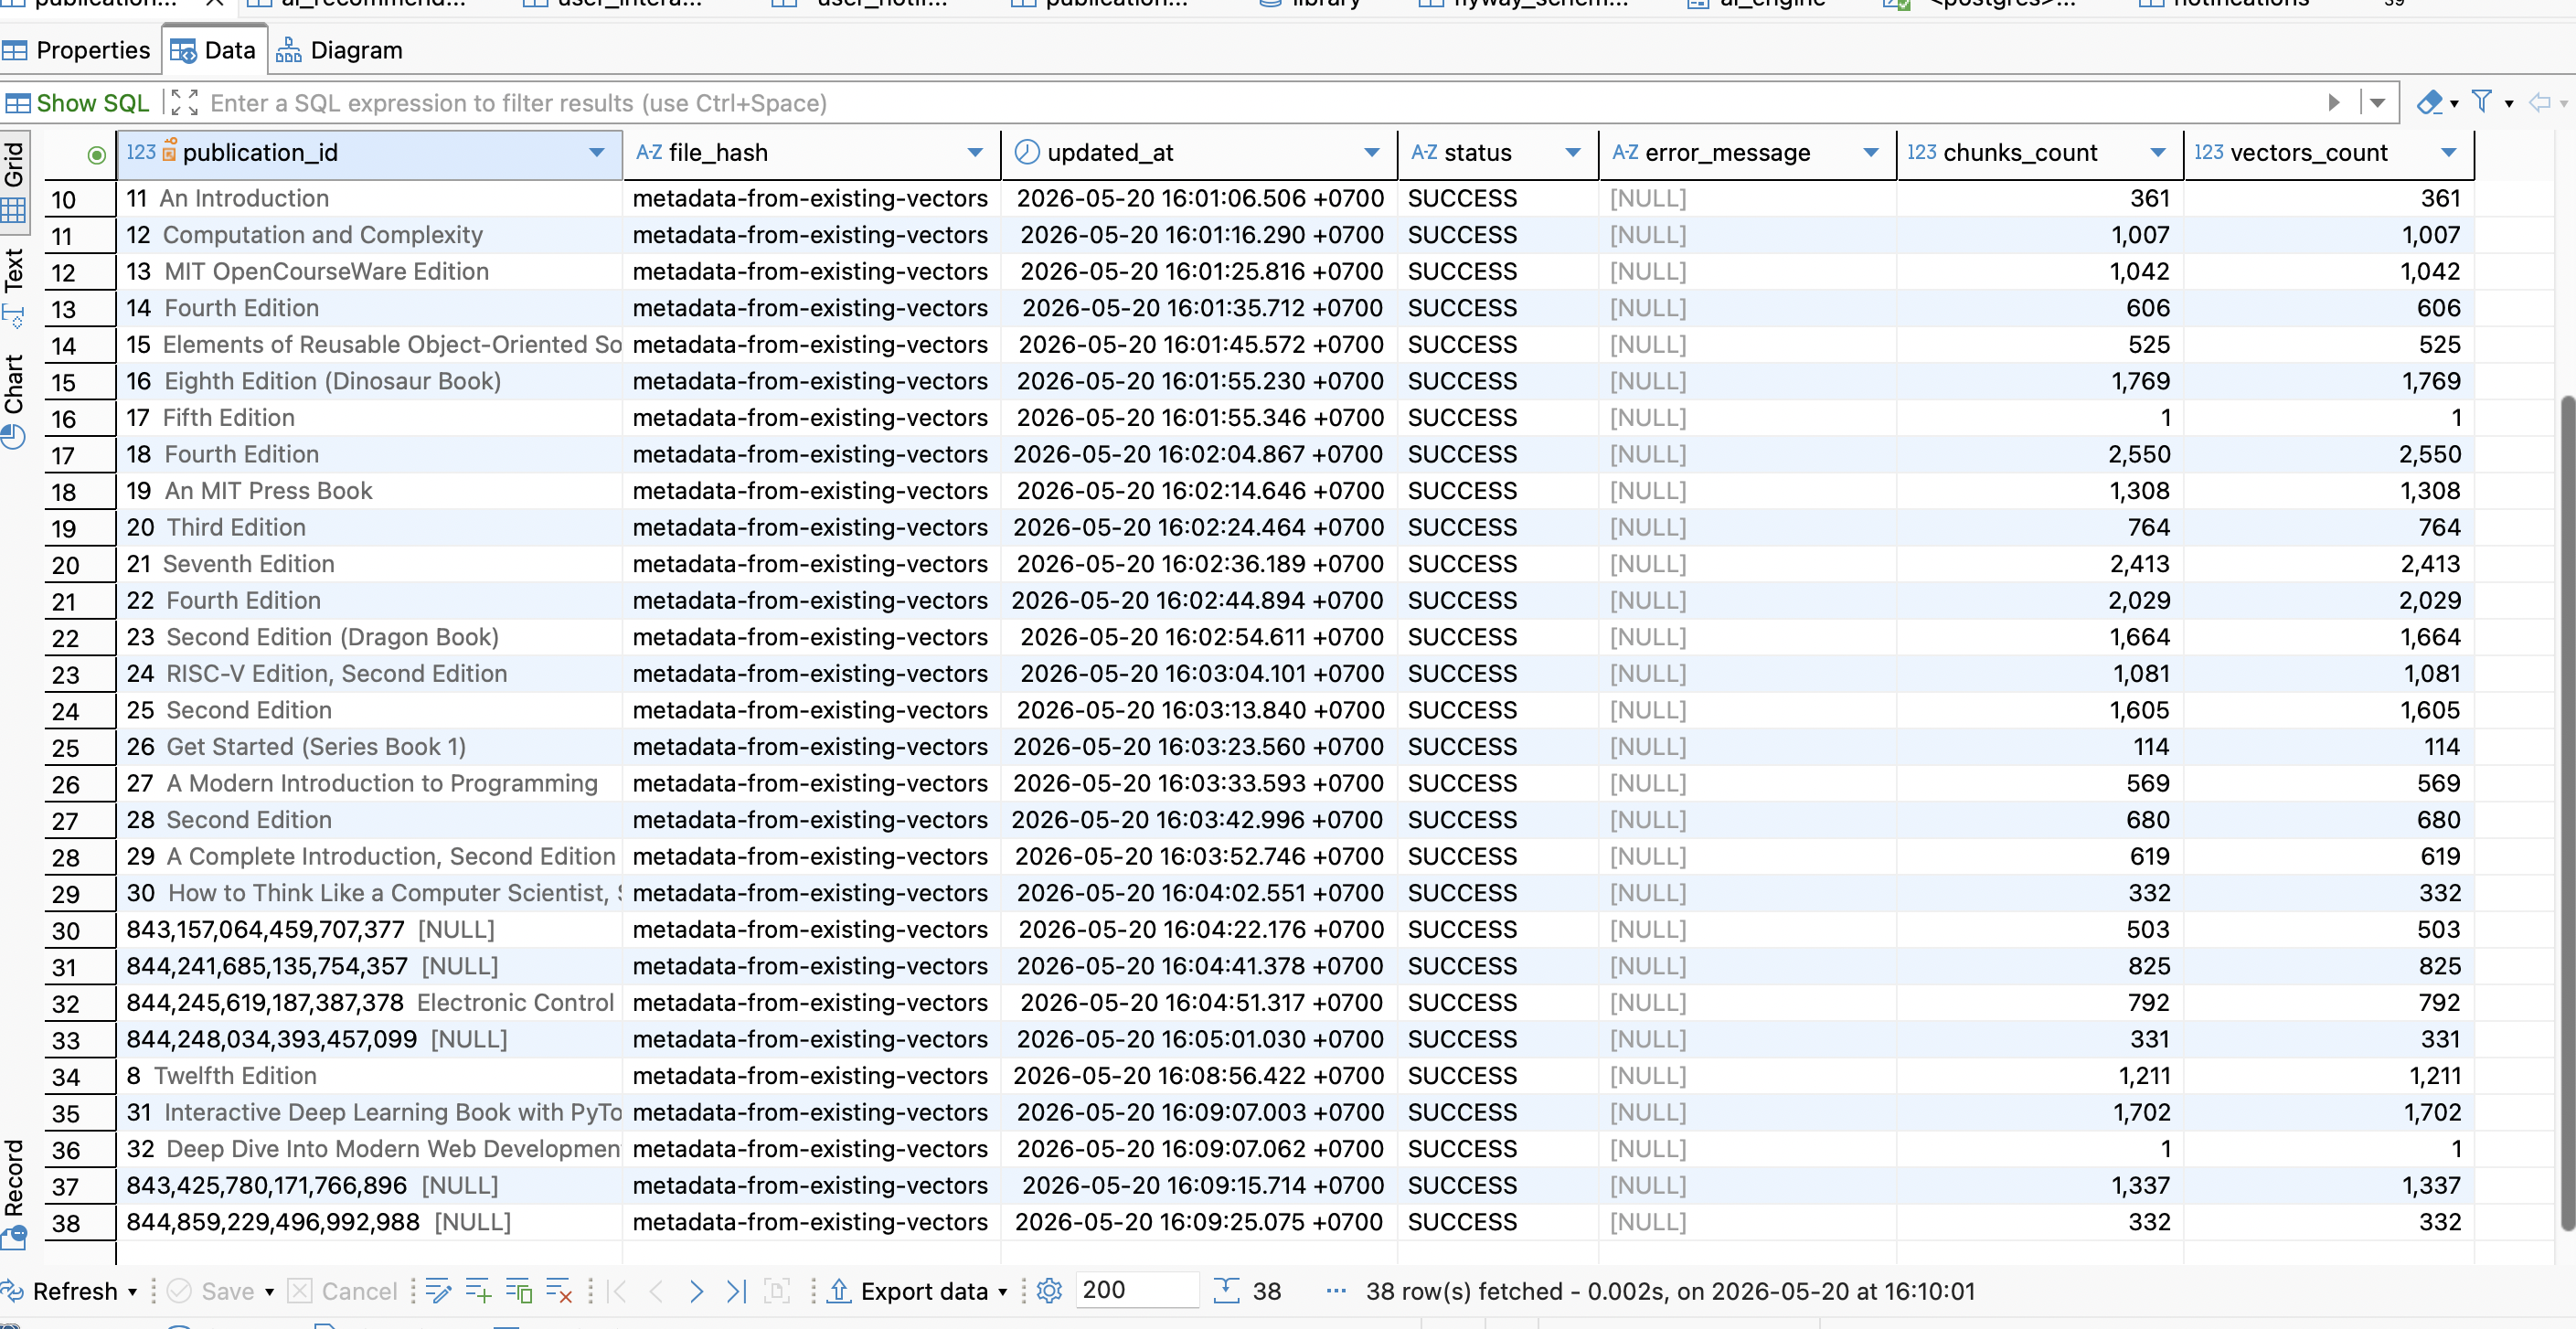
\includegraphics[width=\linewidth]{figures/ch06/ai/etl_run.png}
        \caption{Kết quả chạy ETL}
    \end{subfigure}
    \hfill
    \begin{subfigure}[b]{0.48\textwidth}
        \centering
        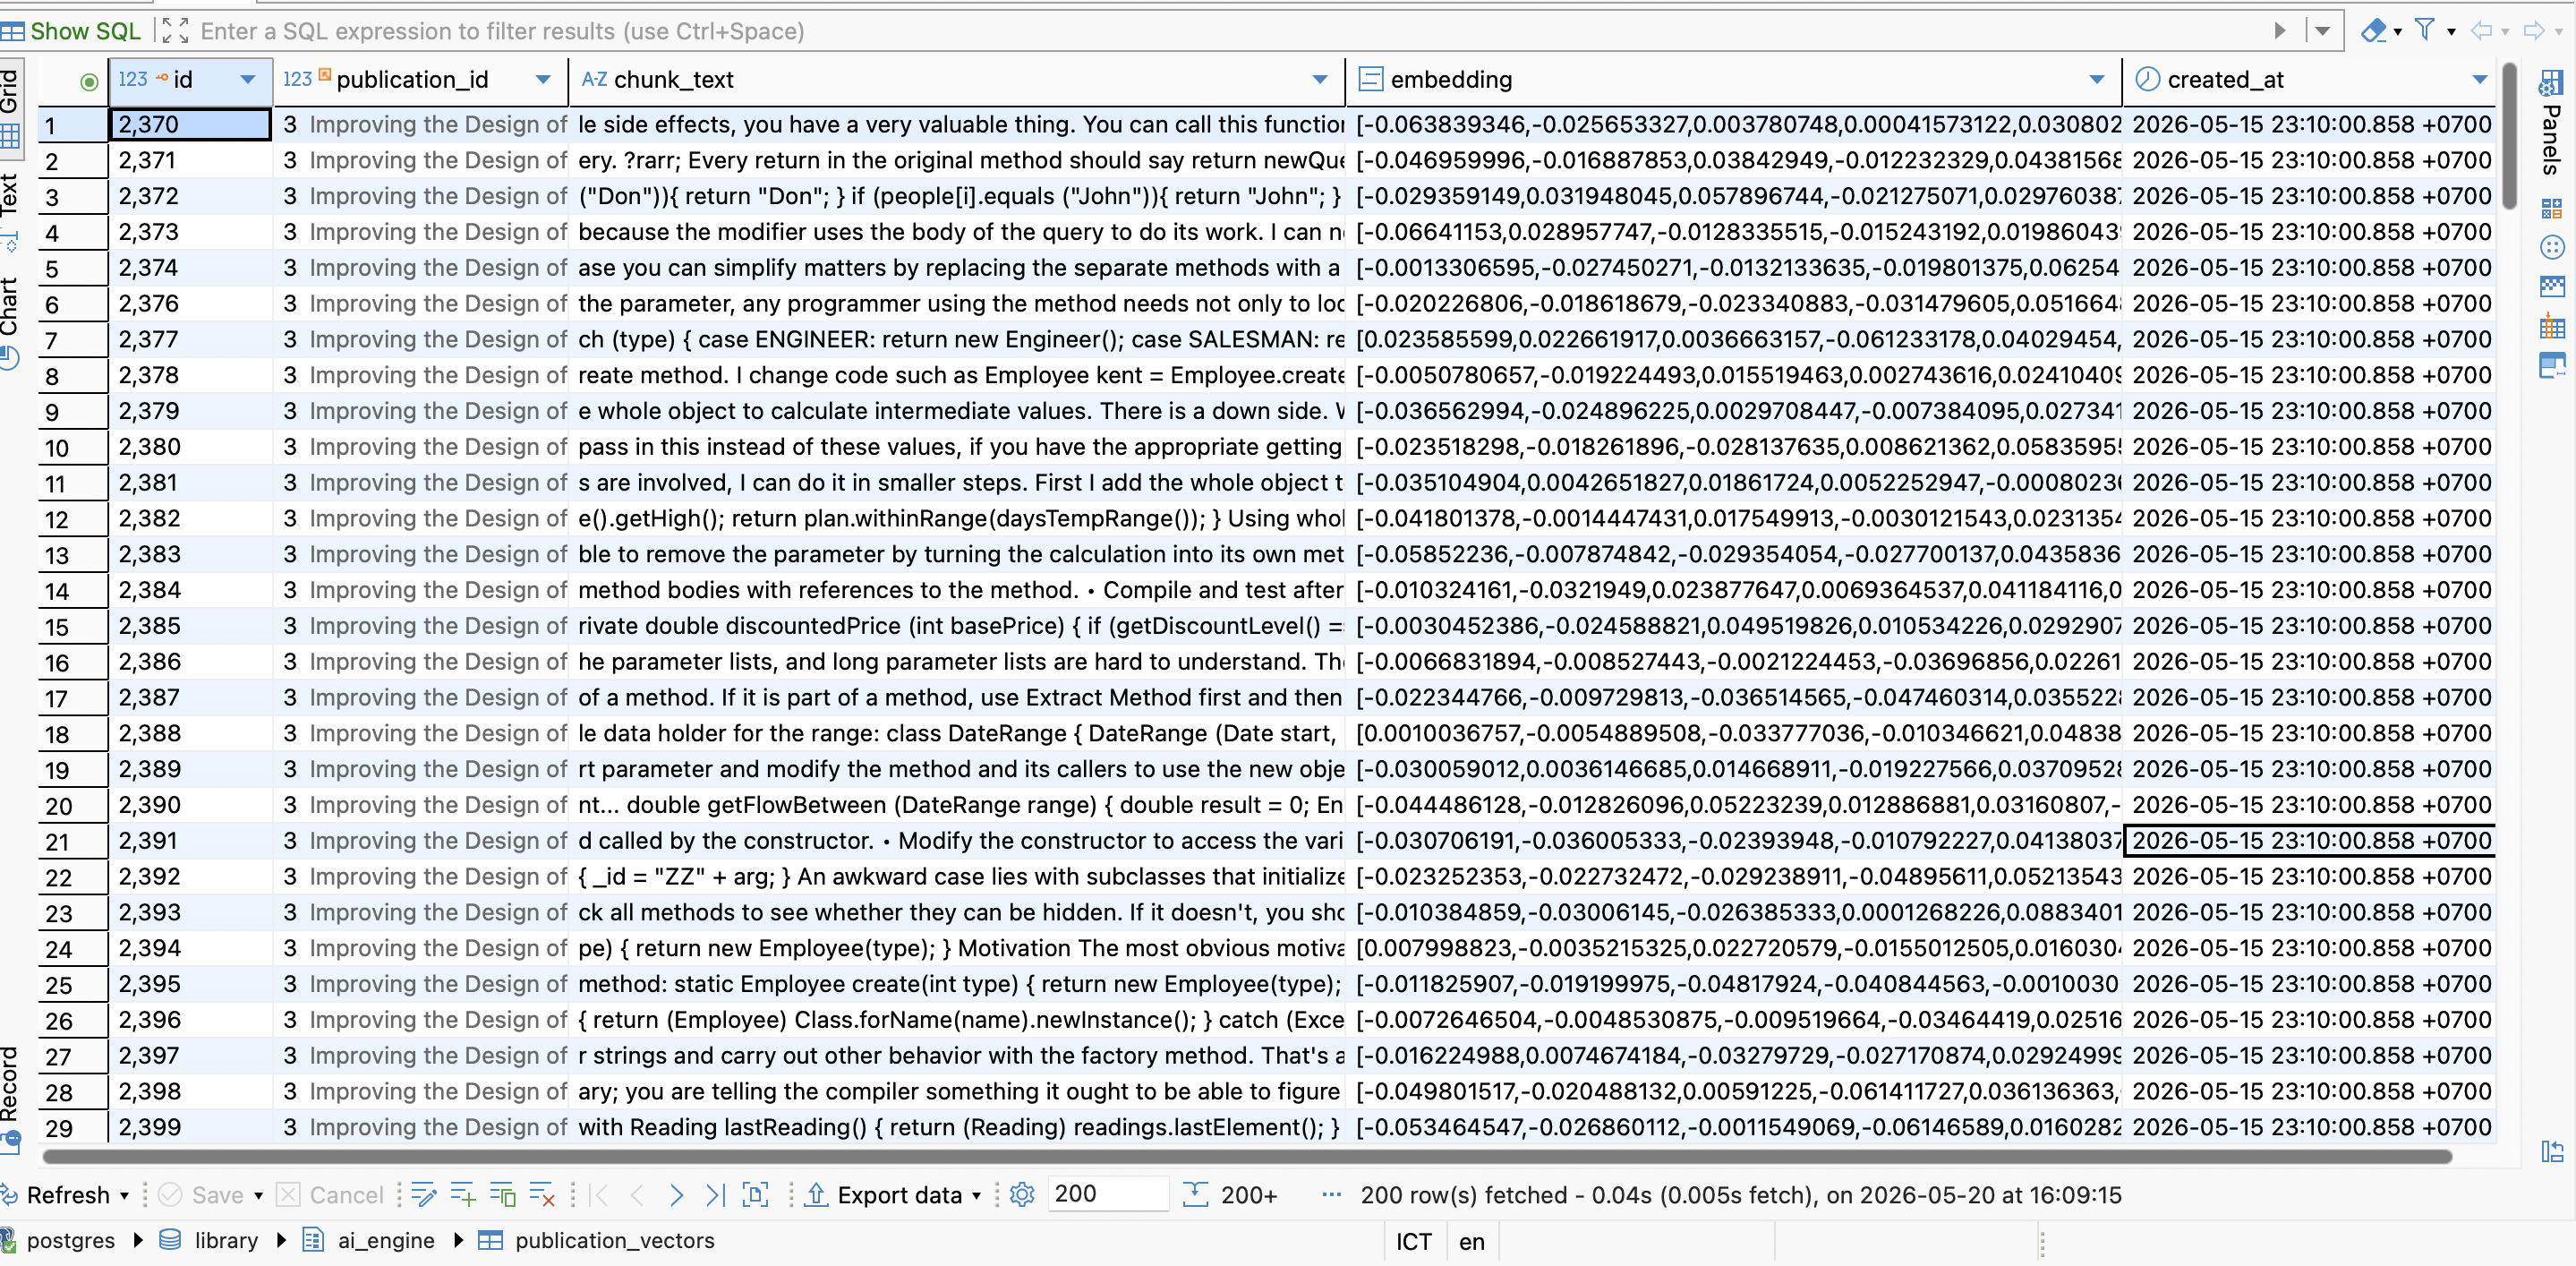
\includegraphics[width=\linewidth]{figures/ch06/ai/vector_db.png}
        \caption{Dữ liệu vector trong PostgreSQL}
    \end{subfigure}
    \caption{Pipeline xử lý PDF và lưu vector}
    \label{fig:ai_etl_vector_showcase}
\end{figure}

% --- ĐOẠN CHUYỂN Ý 2: TỪ HÌNH ẢNH SANG NĂNG LỰC KỸ THUẬT ---
Dựa trên các kết quả trực quan này, Bảng \ref{tab:ai_capability_summary} tổng hợp chi tiết các năng lực trí tuệ nhân tạo cốt lõi mà phân hệ AI Service đã đảm nhiệm. Các năng lực này được thiết kế không chỉ để phô diễn công nghệ, mà còn phải đáp ứng nghiêm ngặt các tiêu chuẩn về an toàn tích hợp, khả năng chịu lỗi (fault tolerance) và cơ chế dự phòng (fallback) khi giao tiếp với mô hình ngôn ngữ lớn (LLM).

\begin{table}[H]
\centering
\small
\begin{tabularx}{\textwidth}{|p{3.5cm}|X|}
\hline
\textbf{Năng lực AI} & \textbf{Nội dung đã hiện thực} \\
\hline
Xử lý PDF &
Upload PDF từ thủ thư, chạy ETL nền, lưu trạng thái \texttt{RUNNING},
\texttt{SUCCESS}, \texttt{FAILED}, không làm gián đoạn nghiệp vụ catalog. \\
\hline
Semantic search &
Sinh embedding cho truy vấn, tìm chunk gần nhất bằng pgvector, gom về
publication id và trả kết quả cho backend lọc nghiệp vụ. \\
\hline
Metadata enrichment &
Sinh summary, audience, tag học thuật, alias tiếng Anh và ghi về publication để
hiển thị trên chi tiết sách/tìm kiếm. \\
\hline
Similar books &
Tính tương đồng dựa trên vector nội dung và metadata để đề xuất sách liên quan
từ trang chi tiết. \\
\hline
Recommendation &
Gợi ý cá nhân hóa theo lịch sử xem, wishlist, mượn, rating; có fallback khi
người dùng mới hoặc dữ liệu tương tác còn ít. \\
\hline
An toàn tích hợp &
Callback HMAC, timeout/retry, fallback local khi LLM lỗi, kiểm thử API contract
và kiểm tra độ trễ cơ bản. \\
\hline
\end{tabularx}
\caption{Các năng lực AI đã tích hợp vào hệ thống}
\label{tab:ai_capability_summary}
\end{table}

% --- ĐOẠN CHUYỂN Ý 3: TỪ KỸ THUẬT SANG GIÁ TRỊ VẬN HÀNH ---
Công nghệ chỉ thực sự có ý nghĩa khi nó phục vụ đúng bài toán con người. Bảng \ref{tab:ai_value_highlights} đúc kết những điểm sáng nổi bật nhất, minh chứng cho việc ứng dụng AI đã thực sự giải phóng sức lao động của thủ thư (thông qua tự động hóa xử lý nền) và nâng tầm trải nghiệm khám phá tri thức của độc giả (thông qua tìm kiếm trên lõi nội dung thay vì từ khóa bề mặt).

\begin{table}[H]
\centering
\small
\begin{tabularx}{\textwidth}{|p{3.4cm}|X|p{3.4cm}|}
\hline
\textbf{Điểm hiện thực} & \textbf{Nội dung đã làm} & \textbf{Giá trị thực tế} \\
\hline
Xử lý nền &
AI worker nhận request, tải PDF, chạy ETL và callback kết quả về backend. &
Thủ thư không phải chờ AI xử lý xong mới tiếp tục thao tác catalog. \\
\hline
Tìm trên nội dung PDF &
Chunk nội dung được embedding và lưu vào pgvector để semantic search. &
Kết quả tìm kiếm dựa trên nội dung sách, không chỉ tiêu đề hoặc mô tả. \\
\hline
Metadata enrichment &
Sinh summary, audience, tag tiếng Việt và alias tiếng Anh. &
Trang chi tiết sách và bộ lọc tìm kiếm có thêm dữ liệu có ích cho người đọc. \\
\hline
Fallback &
Khi LLM lỗi hoặc dữ liệu tương tác ít, hệ thống dùng rule local, content-based và trending. &
Tính năng AI vẫn có kết quả ổn định trong điều kiện demo hoặc quota giới hạn. \\
\hline
\end{tabularx}
\caption{Các điểm giá trị nổi bật ở AI Service}
\label{tab:ai_value_highlights}
\end{table}

% --- ĐOẠN CHUYỂN Ý 4: TỔNG KẾT TOÀN BỘ CHƯƠNG 6 ---
\subsection{Tổng kết kết quả hiện thực}

Khép lại toàn bộ quá trình triển khai từ Frontend, Backend đến AI Service, sự thành công của một hệ thống phần mềm không chỉ nằm ở việc hoàn thiện từng module đơn lẻ, mà là khả năng liên kết chúng thành các luồng nghiệp vụ (Business Flows) thông suốt.

Bảng \ref{tab:implementation_value_flows} tổng hợp 4 luồng giá trị xương sống của dự án, đối chiếu trực tiếp giữa các thành phần công nghệ đã tham gia và những minh chứng rõ nét đã được trình bày xuyên suốt chương này. Đây là thước đo cuối cùng khẳng định hệ thống đã được xây dựng hoàn chỉnh từ đầu đến cuối (end-to-end) và đáp ứng trọn vẹn bài toán thực tiễn đặt ra ban đầu.

\begin{table}[H]
\centering
\small
\begin{tabularx}{\textwidth}{|p{3.4cm}|X|p{3.4cm}|}
\hline
\textbf{Luồng được show} & \textbf{Thành phần tham gia} & \textbf{Kết quả thể hiện trong Chương 6} \\
\hline
Upload và xử lý sách &
Frontend upload, Backend catalog/AI gateway, AI worker, pgvector. &
Có màn hình upload, bảng module, ảnh ETL, ảnh vector DB và callback. \\
\hline
Tìm kiếm thông minh &
Public search UI, Backend search API, AI semantic search, catalog filter. &
Có màn hình tìm kiếm, bảng năng lực AI và ảnh semantic search. \\
\hline
Mượn--trả và thanh toán &
User/librarian UI, circulation module, PayOS, notification realtime. &
Có màn hình dashboard, mượn sách, QR PayOS, cập nhật thanh toán và notification. \\
\hline
Quản trị vận hành &
Admin/librarian pages, audit/policy, scheduler, API documentation. &
Có bảng module Backend, bảng giá trị Backend và ảnh Swagger/cấu trúc module. \\
\hline
\end{tabularx}
\caption{Các luồng giá trị được minh chứng trong phần hiện thực}
\label{tab:implementation_value_flows}
\end{table}

\section{Tổng kết hiện thực}

Về tổng thể, nhóm đã hiện thực hệ thống theo đúng ba lớp: frontend phục vụ tương
tác theo vai trò, backend giữ nghiệp vụ và dữ liệu gốc, AI service xử lý các tác
vụ thông minh. Các chức năng đã làm không chỉ dừng ở demo giao diện, mà đã nối
tới API, cơ sở dữ liệu, tác vụ nền, dịch vụ ngoài, kiểm thử và cấu hình triển
khai. Bảng dưới đây tóm tắt các luồng end-to-end quan trọng nhất.

\begin{table}[H]
\centering
\small
\begin{tabularx}{\textwidth}{|p{3.7cm}|X|}
\hline
\textbf{Luồng end-to-end} & \textbf{Các phần đã nối thông} \\
\hline
Đăng ký/đăng nhập &
Frontend auth pages, backend auth module, email verification, JWT/refresh token,
Google OAuth2 và route guard theo role. \\
\hline
Tra cứu và mượn sách &
Public/user search, catalog API, trạng thái bản sao, circulation API, thông báo
cho bạn đọc và dashboard thủ thư. \\
\hline
Đặt trước &
User reservation page, backend reservation queue, scheduler deadline, xác nhận
nhận sách và notification realtime. \\
\hline
Phí phạt &
Fine API, giao diện bạn đọc/thủ thư, PayOS QR, thanh toán tiền mặt, cập nhật
trạng thái fine và lịch sử giao dịch. \\
\hline
Upload PDF và AI &
Librarian upload, presigned URL, backend AI gateway, worker ETL, Gemini metadata,
pgvector và callback cập nhật publication. \\
\hline
Tìm kiếm/gợi ý thông minh &
Semantic search UI, AI service, recommendation module, behavior tracking, similar
books và fallback khi dữ liệu ít. \\
\hline
Vận hành &
Admin policy, audit log, scheduler, WebSocket notification, Docker Compose,
Nginx reverse proxy và cấu hình môi trường production. \\
\hline
\end{tabularx}
\caption{Các luồng end-to-end đã hiện thực}
\label{tab:end_to_end_summary}
\end{table}
